\documentclass[12pt, a4paper, oneside]{memoir}

%%%%%%%%%%%%%%%% 引入 package %%%%%%%%%%%%%%%%
\usepackage[margin=3cm]{geometry}
\usepackage{amsmath,amsthm,amssymb} % 引入 AMS 數學環境
\usepackage{yhmath}			% math symbol
\usepackage{graphicx}		% 圖形插入用
%\graphicspath{{images/}}	% 搜尋圖片目錄
%\usepackage{wrapfig}		% 文繞圖
\usepackage{floatflt}		% 浮動 figure
%\usepackage{float}			% 浮動環境
%\usepackage{subfig}		% subfigures
%\usepackage{caption3}		% caption 增強
%\usepackage{setspace}   	% 控制空行
\usepackage{fontspec}		% 設定字體
\usepackage{type1cm}		% 設定fontsize
\usepackage{titlesec}		% 設定section等的字體
\usepackage{titling}		% 加強 title 功能
\usepackage{fancyhdr}		% 頁首頁尾
\usepackage{tabularx}		% 加強版 table
\usepackage{listings}		% 內嵌程式碼
\usepackage{indentfirst}	% 首行縮排
\usepackage{enumerate}		% 加強 enumerate
\usepackage{upquote}		% verbatim 中引號顯示
\usepackage{ulem}			% 裝飾
\usepackage{enumitem}
\usepackage[square, comma, numbers, super, sort&compress]{natbib}
\usepackage[unicode=true, pdfborder={0 0 0}, bookmarksdepth=-1]{hyperref}
\usepackage[usenames, dvipsnames]{color}
\usepackage[many]{tcolorbox}

\usepackage{tikz} %繪圖用
\usetikzlibrary{calc,trees,positioning,arrows,chains,shapes.geometric,%
    decorations.pathreplacing,decorations.pathmorphing,shapes,%
    matrix,shapes.symbols}
\usepackage{forest}

\usepackage{xeCJK}  % xelatex 中文
%設定標楷體為中文字型,而英文不去更動,使用原TeX字型
\setCJKmainfont[AutoFakeBold=3,AutoFakeSlant=.4]{Noto Sans CJK TC Regular}
\defaultCJKfontfeatures{AutoFakeBold=3,AutoFakeSlant=.4}
\XeTeXlinebreaklocale "zh"
\XeTeXlinebreakskip = 0pt plus 1pt
\setmonofont{Consolas}

%%%%%%%%%%%%%%%% 頁面設定 %%%%%%%%%%%%%%%%
\setlength{\headheight}{15pt}  %with titling
\setlength{\droptitle}{-1.5cm} %title 與上緣的間距
\parindent=24pt %設定縮排的距離

\fancyhf{}
\fancyhead[L]{\rightmark}
\fancyhead[R]{\thepage}	
\renewcommand{\headrulewidth}{0.4pt}
\renewcommand{\footrulewidth}{0.4pt}
\pagestyle{fancy}

%%%%%%%%%%%%%%%% chapter 樣式 %%%%%%%%%%%%%%%%
\usepackage{calc}\makechapterstyle{combined}{ \setlength{\midchapskip}{-60pt} \setlength{\afterchapskip}{2.5cm} \renewcommand*{\printchaptername}{\thispagestyle{fancy}} \renewcommand*{\chapnumfont}{\normalfont\sffamily\bfseries\fontsize{80}{0}\selectfont} \renewcommand*{\printchapternum}{\flushright\chapnumfont\textcolor[rgb]{.64,.79,.87}{\thechapter}} \renewcommand*{\chaptitlefont}{\normalfont\sffamily\Huge\bfseries} \renewcommand*{\printchaptertitle}[1]{ \raggedright\chaptitlefont\parbox[t]{\textwidth-3cm}{\raggedright##1}} } \chapterstyle{combined} \tcbuselibrary{skins,raster}

%%%%%%%%%%%%%%%% custom environment %%%%%%%%%%%%%%%%
%%%%%%%%%%%%%%%% 內嵌程式碼環境(cpp) %%%%%%%%%%%%%%%%
%\makeatletter
\definecolor{darkgray}{rgb}{0.25, 0.25, 0.25}
\definecolor{editorGray}{rgb}{0.95, 0.95, 0.95}
\definecolor{editorOcher}{rgb}{1, 0.5, 0} % #FF7F00 -> rgb(239, 169, 0)
\definecolor{editorGreen}{rgb}{0, 0.5, 0} % #007C00 -> rgb(0, 124, 0)
\definecolor{editorYellow}{RGB}{255,230,80}
\definecolor{orange}{rgb}{1,0.45,0.13}

\definecolor{magenta}{RGB}{255,0,128}
\definecolor{preprocessor}{RGB}{0,160,0}
\definecolor{primaryKeywords}{RGB}{0,0,160}
\definecolor{secondaryKeywords}{RGB}{0,128,0}
\definecolor{numbers}{RGB}{255,0,0}

\lstdefinestyle{vivid} {%
	% General design
%	backgroundcolor=\color{editorGray},
	basicstyle={\small\ttfamily},   
	frame=tb,
%	autodedent = true,
	% line-numbers
	xleftmargin={0.75cm},
	numbers=left,
	numberstyle=\scriptsize\ttfamily\color{gray},
	stepnumber=1,
	firstnumber=1,
	numberfirstline=true,
	% Code design
	identifierstyle=\color{black},
	keywordstyle={\color{primaryKeywords}},
	keywordstyle={[2]{\color{primaryKeywords}}},
	keywordstyle={[3]{\color{secondaryKeywords}}},
	keywordstyle={[4]{\color{magenta}}},
	stringstyle=\color{editorOcher}\ttfamily,
	% Code
	% alsodigit={.:;},	
	tabsize=4,
	showtabs=false,
	showspaces=false,
	showstringspaces=false,
	extendedchars=true,
	breaklines=true,
	captionpos=b,
}
\lstdefinestyle{bw} {%
	% General design
	backgroundcolor=\color{editorGray},
	basicstyle={\small\ttfamily},   
	frame=tb,
	% line-numbers
%	xleftmargin={0.75cm},
	numbers=left,
	numberstyle=\scriptsize\ttfamily,
	stepnumber=1,
	firstnumber=1,
	numberfirstline=true,	
	% Code design
	identifierstyle=\ttfamily,
	keywordstyle=\bfseries,
	commentstyle=\color{gray}\ttfamily,
	% Code
	%alsodigit={.:;},
	tabsize=4,
	showtabs=false,
	showspaces=false,
	showstringspaces=false,
	extendedchars=true,
	breaklines=true,
	captionpos=b,
}
\iffalse
	literate=%
% numbers
{0}{{{\color{numbers}0}}}1
{1}{{{\color{numbers}1}}}1
{2}{{{\color{numbers}2}}}1
{3}{{{\color{numbers}3}}}1
{4}{{{\color{numbers}4}}}1
{5}{{{\color{numbers}5}}}1
{6}{{{\color{numbers}6}}}1
{7}{{{\color{numbers}7}}}1
{8}{{{\color{numbers}8}}}1
{9}{{{\color{numbers}9}}}1
% operator
{\ *\ }{{{\color{magenta}\ *\ }}}{1}
{\ /\ }{{{\color{magenta}\ /\ }}}{1}
{!}{{{\color{magenta}!}}}{1}
{(}{{{\color{magenta}(}}}{1}
{)}{{{\color{magenta})}}}{1}
{+}{{{\color{magenta}+}}}{1}
{-}{{{\color{magenta}-}}}{1}
{,}{{{\color{magenta},}}}{1}
{.}{{{\color{magenta}.}}}{1}
{:}{{{\color{magenta}:}}}{1}
{<}{{{\color{magenta}<}}}{1}
{=}{{{\color{magenta}=}}}{1}
{>}{{{\color{magenta}>}}}{1}
{?}{{{\color{magenta}?}}}{1}
{[}{{{\color{magenta}[}}}{1}
{]}{{{\color{magenta}]}}}{1}
{|}{{{\color{magenta}|}}}{1}
{;}{{{\color{magenta};}}}{1}
{\^{}}{{{\color{magenta}\^{}}}}{1}
{\~{}}{{{\color{magenta}\~{}}}}{1}
{\%}{{{\color{magenta}\%}}}{1}
{\&}{{{\color{magenta}\&}}}{1}
{\{}{{{\color{magenta}\{}}}{1}
{\}}{{{\color{magenta}\}}}}{1},
\fi
\lstdefinelanguage{cppcodeblocks}{
	language=C++,
	sensitive=true,
	morecomment=[l][\color{preprocessor}]{\#},
	morecomment=[l][\color{gray}]{//}, % l for line comment
	morecomment=[s][\color{gray}]{/*}{*/}, % s for start and end delimiter
	morestring=[b]", % b for brackets style
	morestring=[b]',
	morekeywords=[2]{
% primary keywords
alignas, alignof, asm, auto, bool, break, case, catch, char, char16\_t, char32\_t, class, const, const\_cast, constexpr, continue, decltype, default, delete, do, double, dynamic\_cast, else, enum, explicit, export, extern, false, final, float, for, friend, goto, if, inline, int, long, mutable, namespace, new, noexcept, nullptr, operator, override, private, protected, public, register, reinterpret\_cast, return, short, signed, sizeof, static, static\_assert, static\_cast, struct, switch, template, this, thread\_local, throw, true, try, typedef, typeid, typename, union, unsigned, using, virtual, void, volatile, wchar\_t, while, int8\_t, uint8\_t, int16\_t, uint16\_t, int32\_t, uint32\_t, int64\_t, uint64\_t, int\_least8\_t, uint\_least8\_t, int\_least16\_t, uint\_least16\_t, int\_least32\_t, uint\_least32\_t, int\_least64\_t, uint\_least64\_t, int\_fast8\_t, uint\_fast8\_t, int\_fast16\_t, uint\_fast16\_t, int\_fast32\_t, uint\_fast32\_t, int\_fast64\_t, uint\_fast64\_t, intptr\_t, uintptr\_t, intmax\_t, uintmax\_t, wint\_t, wchar\_t, wctrans\_t, wctype\_t, size\_t, time\_t, 
	},
	morekeywords=[3]{
% secondary keywords(STL)
\_\_gnu\_cxx, accumulate, add\_const, add\_cv, add\_lvalue\_reference, add\_pointer, add\_reference, add\_rvalue\_reference, add\_volatile, adjacent\_difference, adjacent\_find, aligned\_storage, Alignment, alignment\_of, all\_of, allocate\_shared, allocator, allocator\_base, allocator\_chunklist, allocator\_fixed\_size, allocator\_newdel, allocator\_suballoc, allocator\_unbounded, allocator\_variable\_size, any\_of, array, assign, at, atomic\_bool, atomic\_char, atomic\_char16\_t, atomic\_char32\_t, atomic\_compare\_exchange\_strong, atomic\_compare\_exchange\_strong\_explicit, atomic\_compare\_exchange\_weak, atomic\_compare\_exchange\_weak\_explicit, atomic\_exchange, atomic\_exchange\_explicit, atomic\_fetch\_add, atomic\_fetch\_and, atomic\_fetch\_or, atomic\_fetch\_sub, atomic\_fetch\_xor, atomic\_int, atomic\_int\_fast16\_t, atomic\_int\_fast32\_t, atomic\_int\_fast64\_t, atomic\_int\_fast8\_t, atomic\_int\_least16\_t, atomic\_int\_least32\_t, atomic\_int\_least64\_t, atomic\_int\_least8\_t, atomic\_intmax\_t, atomic\_intptr\_t, atomic\_is\_lock\_free, atomic\_llong, atomic\_load, atomic\_load\_explicit, atomic\_long, atomic\_ptrdiff\_t, atomic\_schar, atomic\_short, atomic\_size\_t, atomic\_ssize\_t, atomic\_store, atomic\_store\_explicit, atomic\_uchar, atomic\_uint, atomic\_uint\_fast16\_t, atomic\_uint\_fast32\_t, atomic\_uint\_fast64\_t, atomic\_uint\_fast8\_t, atomic\_uint\_least16\_t, atomic\_uint\_least32\_t, atomic\_uint\_least64\_t, atomic\_uint\_least8\_t, atomic\_uintmax\_t, atomic\_uintptr\_t, atomic\_ullong, atomic\_ulong, atomic\_ushort, atomic\_wchar\_t, auto\_ptr, back, back\_insert\_iterator, back\_item, bad\_alloc, bad\_function\_call, bad\_weak\_ptr, basic\_filebuf, basic\_fstream, basic\_ifstream, basic\_ofstream, basic\_regex, basic\_streambuf, basic\_string, begin, bernoulli\_distribution, bidirectional\_iterator\_tag, binary\_function, binary\_negate, binary\_search, bind, bind1st, bind2nd, binder1st, binder2nd, binomial\_distribution, bit\_and, bit\_or, bit\_xor, bitset, boost, cache\_chunklist, cache\_freelist, cache\_suballoc, cauchy\_distribution, cbegin, cend, cerr, char\_traits, checked\_array\_iterator, checked\_uninitialized\_copy, checked\_uninitialized\_fill\_n, chi\_squared\_distribution, cin, clear, codecvt, codecvt\_base, codecvt\_byname, codecvt\_mode, codecvt\_utf16, codecvt\_utf8, codecvt\_utf8\_utf16, collate, collate\_byname, common\_type, compare\_exchange\_strong, compare\_exchange\_weak, complex, condition\_variable, conditional, const\_iterator, const\_mem\_fun\_ref\_t, const\_mem\_fun\_t, const\_mem\_fun1\_ref\_t, const\_mem\_fun1\_t, const\_pointer\_cast, const\_reference, const\_reverse\_iterator, copy, copy\_backward, copy\_if, copy\_n, count, count\_if, cout, crbegin, cref, crend, ctype, ctype\_base, ctype\_byname, decay, declare\_no\_pointers, declare\_reachable, declval, default\_delete, default\_random\_engine, deque, difference\_type, discard\_block, discard\_block\_engine, discrete\_distribution, divides, domain\_error, dynamic\_pointer\_cast, empty, enable\_if, enable\_shared\_from\_this, end, endl, equal, equal\_range, equal\_to, EqualityComparable, erase, error\_category, error\_code, error\_condition, exception, exponential\_distribution, extent, extreme\_value\_distribution, fetch\_add, fetch\_and, fetch\_or, fetch\_sub, fetch\_xor, filebuf, fill, fill\_n, find, find\_end, find\_first\_of, find\_first\_not\_of, find\_if, find\_if\_not, find\_last\_of, find\_last\_not\_of, fisher\_f\_distribution, float\_denorm\_style, float\_round\_style, for\_each, forward, forward\_iterator\_tag, forward\_list, freelist, front, front\_insert\_iterator, front\_item, fstream, function, gamma\_distribution, generate, generate\_n, generic\_container, generic\_iterator, generic\_reverse\_iterator, generic\_value, geometric\_distribution, get\_deleter, get\_pointer\_safety, get\_temporary\_buffer, greater, greater\_equal, has\_nothrow\_assign, has\_nothrow\_constructor, has\_nothrow\_copy, has\_nothrow\_copy\_assign, has\_nothrow\_copy\_constructor, has\_nothrow\_default\_constructor, has\_trivial\_assign, has\_trivial\_constructor, has\_trivial\_copy, has\_trivial\_copy\_assign, has\_trivial\_copy\_constructor, has\_trivial\_default\_constructor, has\_trivial\_destructor, has\_virtual\_destructor, hash, hash\_map, hash\_set, ifstream, includes, independent\_bits\_engine, initializer\_list, inner\_product, inplace\_merge, input\_iterator\_tag, insert, insert\_iterator, integral\_constant, invalid\_argument, ios\_base, iostream, is\_abstract, is\_arithmetic, is\_array, is\_base\_of, is\_bind\_expression, is\_class, is\_compound, is\_const, is\_constructible, is\_convertible, is\_empty, is\_enum, is\_error\_code\_enum, is\_error\_condition\_enum, is\_explicitly\_convertible, is\_floating\_point, is\_function, is\_fundamental, is\_heap, is\_heap\_until, is\_integral, is\_literal\_type, is\_lock\_free, is\_lvalue\_reference, is\_member\_function\_pointer, is\_member\_object\_pointer, is\_member\_pointer, is\_nothrow\_constructible, is\_object, is\_partitioned, is\_placeholder, is\_pod, is\_pointer, is\_polymorphic, is\_reference, is\_rvalue\_reference, is\_same, is\_scalar, is\_signed, is\_sorted, is\_sorted\_until, is\_standard\_layout, is\_trivial, is\_union, is\_unsigned, is\_void, is\_volatile, istream, istream\_iterator, istreambuf\_iterator, iter\_swap, iterator, iterator\_traits, knuth\_b, length\_error, less, less\_equal, LessThanComparable, lexicographical\_compare, linear\_congruential, linear\_congruential\_engine, list, locale, logic\_error, logical\_and, logical\_not, logical\_or, lognormal\_distribution, lower\_bound, make\_checked\_array\_iterator, make\_heap, make\_shared, make\_signed, make\_unsigned, map, match\_results, max, max\_element, max\_fixed\_size, max\_none, max\_unbounded, max\_variable\_size, mem\_fn, mem\_fun, mem\_fun\_ref, mem\_fun\_ref\_t, mem\_fun\_t, mem\_fun1\_ref\_t, mem\_fun1\_t, merge, mersenne\_twister, mersenne\_twister\_engine, messages, messages\_base, messages\_byname, min, min\_element, minmax, minmax\_element, minstd\_rand, minstd\_rand0, minus, mismatch, modulus, money\_base, money\_get, money\_put, moneypunct, moneypunct\_byname, move, move\_backward, move\_iterator, mt19937, mt19937\_64, multimap, multiplies, multiset, negate, negative\_binomial\_distribution, new\_handler, next\_permutation, none\_of, normal\_distribution, not\_equal\_to, not1, not2, nothrow, nothrow\_t, npos, nth\_element, num\_get, num\_put, numeric\_limits, numpunct, numpunct\_byname, ofstream, ostream, ostream\_iterator, ostreambuf\_iterator, out\_of\_range, output\_iterator\_tag, overflow\_error, owner\_less, pair, partial\_sort, partial\_sort\_copy, partial\_sum, partition, partition\_copy, partition\_point, piecewise\_constant\_distribution, piecewise\_linear\_distribution, plus, pointer\_safety, pointer\_to\_binary\_function, pointer\_to\_unary\_function, poisson\_distribution, pop\_back, pop\_front, pop\_heap, prev\_permutation, priority\_queue, ptr\_fun, push\_back, push\_front, push\_heap, queue, random\_access\_iterator\_tag, random\_device, random\_shuffle, range\_error, rank, ranlux\_base\_01, ranlux24, ranlux24\_base, ranlux3, ranlux3\_01, ranlux4, ranlux4\_01, ranlux48, ranlux48\_base, ranlux64\_base\_01, ratio, ratio\_add, ratio\_divide, ratio\_multiply, ratio\_subtract, raw\_storage\_iterator, rbegin, rdbuf, ref, reference, reference\_wrapper, regex, regex\_constants, regex\_error, regex\_iterator, regex\_token\_iterator, regex\_traits, remove, remove\_all\_extents, remove\_const, remove\_copy, remove\_copy\_if, remove\_cv, remove\_extent, remove\_if, remove\_pointer, remove\_reference, remove\_volatile, rend, replace, replace\_copy, replace\_copy\_if, replace\_if, requires, resize, result\_of, return\_temporary\_buffer, reverse, reverse\_copy, reverse\_iterator, rotate, rotate\_copy, rts\_alloc, runtime\_error, search, search\_n, seed\_seq, set, set\_difference, set\_intersection, set\_new\_handler, set\_symmetric\_difference, set\_union, setprecision, setw, shared\_ptr, shuffle\_order\_engine, size, size\_type, sort, sort\_heap, stable\_partition, stable\_sort, stack, static\_pointer\_cast, std, streambuf, string, stringstream, student\_t\_distribution, sub\_match, substr, subtract\_with\_carry, subtract\_with\_carry\_01, subtract\_with\_carry\_engine, swap, swap\_ranges, sync\_none, sync\_per\_container, sync\_per\_thread, sync\_shared, system\_error, time\_base, time\_get, time\_get\_byname, time\_put, time\_put\_byname, to\_array, tr1, transform, tuple, tuple\_element, tuple\_size, type\_info, unary\_function, unary\_negate, unchecked\_uninitialized\_copy, unchecked\_uninitialized\_fill\_n, undeclare\_no\_pointers, undeclare\_reachable, underflow\_error, uniform\_int, uniform\_int\_distribution, uniform\_real, uniform\_real\_distribution, uninitialized\_copy, uninitialized\_copy\_n, uninitialized\_fill, uninitialized\_fill\_n, unique, unique\_copy, unique\_ptr, unordered\_map, unordered\_multimap, unordered\_multiset, unordered\_set, upper\_bound, valarray, value\_type, variate\_generator, vector, wcerr, wcin, wcout, weak\_ptr, weibull\_distribution, wfilebuf, wfstream, wifstream, wiostream, wistream, wofstream, wregex, xor\_combine,
	},
%	deletekeywords={(,),\{,\}},
%	otherkeywords=[4]{(,),\{,\}},
}
%\renewcommand\lstlistingname{Sample Code}
\newcommand{\inline}[2][black]{{\color{#1}\ttfamily{#2}}}
%\newcommand{\inline}[1]{{\lstlisting[style=vivid,caption=,language=cppcodeblocks]{#1}}}
%\newcommand{\Cinline}[1]{\lstinline [style=bw, language = cppcodeblocks, keepspaces=true] {#1}}
\lstnewenvironment{C++}[1][]{\lstset{style=vivid, caption = {#1}, language=cppcodeblocks}}{}

\newtcbtheorem[number within=section]{eericbox}{跟著蕭電這樣做}{
	colback=white,colframe=purple,fonttitle=\bfseries,
	enhanced,
	coltitle=white,
	attach boxed title to top left={xshift=2mm,yshift=-2mm,yshifttext=-1mm},
	boxed title style={colframe=purple,colback=purple},
}{th}

\newtcbtheorem[number within=section]{thm}{定理}{
	colback=white,colframe=purple,fonttitle=\bfseries,
	enhanced,
	coltitle=white,
	attach boxed title to top left={xshift=2mm,yshift=-2mm,yshifttext=-1mm},
	boxed title style={colframe=purple, colback=purple},
}{th}

\newtcbtheorem[number within=section]{dfn}{定義}{
	colback=white,colframe=editorGreen,fonttitle=\bfseries,
	enhanced,
	coltitle=white,
	attach boxed title to top left={xshift=2mm,yshift=-2mm,yshifttext=-1mm},
	boxed title style={colframe=editorGreen,colback=editorGreen},
}{th}

\newtcbtheorem[number within=section]{lem}{引理}{
	colback=white,colframe=olive,fonttitle=\bfseries,
	enhanced,
	coltitle=white,
	attach boxed title to top left={xshift=2mm,yshift=-2mm,yshifttext=-1mm},
	boxed title style={colframe=olive, colback=olive},
}{th}

\newtcbtheorem[number within=section]{prbox}{習題}{
	colback=white,colframe=blue!75,fonttitle=\bfseries,
	enhanced,
	coltitle=white,
	attach boxed title to top left={xshift=2mm,yshift=-2mm,yshifttext=-1mm},
	boxed title style={colframe=blue!75,colback=blue!75},
}{th}

\newcommand{\hint}[1]{
	\begin{tcolorbox}[lowerbox=ignored,skin=enhanced,interior style={left color=red!35,right color=white}, colframe = white]
		#1
		\tcblower
	\end{tcolorbox}
}
\newcommand{\definition}[2]{ \begin{dfn}{#1}{} #2 \end{dfn} }
\newcommand{\theorem}[3][]{ \begin{thm}{#2}{#1} #3 \end{thm} }
\newcommand{\eeric}[1]{ \begin{eericbox*}{}{} #1 \end{eericbox*} }
\newcommand{\lemma}[2]{ \begin{lem}{#1}{} #2 \end{lem} }
\newcommand{\problem}[2]{ \begin{prbox}{#1}{} #2 \end{prbox} }

\begin{document}
	%\maketitle %製作tilte page
	%\tableofcontents %目錄
	%%%%%%%%%%%%%%%% \include{filename} %%%%%%%%%%%%%%%%

%	\chapter{基礎圖論}

圖論在演算法這門學科裡佔了十分重要的地位,在競賽中有大約一半的題目會用到圖論的算法與觀念,學著怎麼處理圖,與學習語法一樣重要。\\

\section{名詞解釋}
\subsection{一堆怪東東}

\begin{enumerate}
\item 圖 (Graph):許多頂點與邊的集合,常用 $G(V, E)$ 表示。
\item 頂點 (Vertex):就是頂點 。常用 $v$ 表示。$V$ 就是頂點的集合。
\item 邊 (Edge):連接兩個頂點的東西,可表示成 $e = (u, v)$。$E$ 就是邊的集合。
\item 有向/無向 (Directed/Undirected) 邊:如果 $(u, v)$ 與 $(v, u)$ 代表的是同一條邊,則稱這條邊是無向邊,反之則其中任一條邊為有向邊。
\item 度數 (Degree):一個頂點連接的邊數,即為這個頂點的度數。
\item 入度/出度 (Indegree/Outdegree):若為有向邊,則度數分為入度與出度,分別代表以此頂點為終點與起點的邊數。
\item 鄰接 (Adjacent):如果兩個頂點間有邊連接,則稱這兩個頂點鄰接。
\item 自環:連接相同頂點的邊,即 $(v, v)$。
\item 重邊:兩條或以上連接相同兩個點的邊。
\item 路徑 (Path):一個頂點與邊交錯的序列,滿足每個邊都要連接兩個頂點,且從頂點開始、頂點結束。以 $(v_s, e_1, v_1, e_2, v_2, ..., v_e)$ 表示。
\item 行跡 (Trace):不包含重複邊的路徑。
\item 簡單路徑 (Track):不包含重複頂點的路徑。
\item 迴路 (Circuit):起點與終點為相同頂點的路徑。
\item 環 (Cycle):起點與終點為唯一相同頂點的簡單路徑。
\end{enumerate}

\subsection{各種圖}
\begin{enumerate}
\item 有向圖/無向圖:每條邊都是無向邊的圖稱為無向圖,反之為有向圖。
\item 帶權圖/不帶權圖:有時點上或邊上會有權重,稱為帶權圖。
\item 連通圖:把所有邊變成無向邊後,對於圖上的所有頂點對 $(u, v)$,都存在一個起點為 $u$,終點為 $v$ 的路徑,則稱這個圖為連通圖。
\item 強連通圖:若有向圖上的所有頂點對 $(u, v)$,都存在一個起點為 $u$,終點為 $v$ 的路徑,則稱這個圖為強連通圖。
\item 簡單圖:沒有重邊以及自環的圖,不一定連通。
\item 完全圖:每個頂點都與圖上其他所有頂點鄰接的圖,稱為完全圖。
\item 子圖:今有兩圖 $G(V, E)$ 與 $H$,若對於所有屬於 $H$ 的頂點 $v_i$ 與邊 $e_i$ 皆有 $v_i \in V$ 且 $e_i \in E$ (即 $H$ 內所有頂點與邊都屬於 $G$),則稱 $H$ 是 $G$ 的子圖。
\item 補圖:若圖 $G$ 與圖 $H$ 的頂點集合相同,且兩圖的邊集合聯集為完全圖、交集為空集合,則稱圖 $G$ 與圖 $H$ 互為補圖。
\item 樹:沒有環的連通無向圖稱為樹。
\item 森林:很多樹 (包括一棵) 的聯集稱為森林。
\item 二分圖:如果可以將一張圖的點集分為兩部分,同一部分的任兩點不鄰接,則稱為二分圖。
\item 有向無環圖:簡稱DAG,就是沒有環的有向圖。
\item 稀疏圖/稠密圖:如果邊數十分多(如完全圖),也就是$|E| = O(|V^2|)$,則稱這個圖是稠密圖。若邊數不多($|E| = O(|V|)$ 或 $O(|E|) = O(|V|\log|V|)$),則稱為稀疏圖。
\end{enumerate}

\par 
以上是定義,讓我們看看例圖:

\begin{center}
\begin{tikzpicture}[every node/.style={circle,draw=black}]
\node (v1) at (2*0/3,2*5/3) {$v_0$};
\node (v2) at (2*3/3,2*4/3) {$v_1$};
\node (v3) at (2*6/3,2*5/3) {$v_2$};
\node (v4) at (2*4/3,2*1/3) {$v_3$};
\node (v5) at (2*7/3,2*2/3) {$v_4$};
\draw (v1) -- (v2);
\draw (v2) -- (v3);
\draw (v2) -- (v4);
\draw (v3) -- (v5);
\draw (v4) -- (v5);
\draw (v3) -- (v4);
\draw (v2) -- (v5);

\node (v1) at (2*10/3,2*5/3) {$v_0$};
\node (v2) at (2*13/3,2*4/3) {$v_1$};
\node (v3) at (2*16/3,2*5/3) {$v_2$};
\node (v4) at (2*14/3,2*1/3) {$v_3$};
\node (v5) at (2*17/3,2*2/3) {$v_4$};
\draw[->] (v1) -- (v2);
\draw[->] (v2) -- (v3);
\draw[->] (v2) -- (v4);
\draw[->] (v3) -- (v5);
\draw[->] (v4) -- (v5);
\draw[->] (v3) -- (v4);
\draw[<-] (v2) -- (v5);
\end{tikzpicture}
\end{center}
 
我們常用這種方法表示無向圖與有向圖。圖論中的圖上每條邊都是連接兩個頂點,不會交叉。

\section{圖的儲存}
在學習圖論的時候,看到各式各樣的演算法,一定要先確定這個演算法要用什麼方式把圖存下來會比較好處理。這裡提供了三種把圖存在記憶體裡的方式,各自有各自的優缺利弊,在不同圖論算法上有不同應用。\\

通常測資在輸入一張圖時,會先給定兩個數 $n, m$,分別代表頂點數以及邊數,接下來會有 $m$ 行,每行輸入兩個數字 $u_i, v_i$,代表有一條邊從頂點 $u_i$ 連至頂點 $v_i$,如果是帶權圖,那麼每行會輸入三個數,分別代表兩端點以及權重。\\

讓我們把這種輸入格式轉成方便處理的形式吧!

\subsection{鄰接矩陣 (Adjacency Matrix)}
鄰接矩陣是把圖存下來最直覺的想法。考慮一張無向圖:
\begin{center}
\begin{tikzpicture}[every node/.style={circle,draw=black}]
\node (v1) at (2*0/3,2*5/3) {$v_0$};
\node (v2) at (2*3/3,2*4/3) {$v_1$};
\node (v3) at (2*6/3,2*5/3) {$v_2$};
\node (v4) at (2*4/3,2*1/3) {$v_3$};
\node (v5) at (2*7/3,2*2/3) {$v_4$};
\draw (v1) -- (v2);
\draw (v2) -- (v3);
\draw (v2) -- (v4);
\draw (v3) -- (v5);
\draw (v4) -- (v5);
\draw (v3) -- (v4);
\draw (v2) -- (v5);
\end{tikzpicture}
\end{center}

我們可以將這張圖轉成以下矩陣:
\begin{displaymath}
\begin{bmatrix}
0 & 1 & 0 & 0 & 0\\
1 & 0 & 1 & 1 & 1\\
0 & 1 & 0 & 1 & 1\\
0 & 1 & 1 & 0 & 1\\
0 & 1 & 1 & 1 & 0
\end{bmatrix}
\end{displaymath}

若 $A$ 是一張圖的鄰接矩陣,表示頂點 $i$ 與頂點 $j$ 之間有邊時 $A[i][j] = A[j][i] = 1$,反之 $A[i][j] = 0$。\\

\definition{鄰接矩陣}{
	對於一張圖 $G$,若矩陣 $A$ 滿足:
	\begin{displaymath}
	A[i][j] = 1, \mbox{若邊 $(i, j) \in G$}
	\end{displaymath}
	\begin{displaymath}
	A[i][j] = 0, \mbox{若邊 $(i, j) \notin G$}
	\end{displaymath}
	則稱矩陣 $A$ 是圖 $G$ 的鄰接矩陣。
}

鄰接矩陣也可以處理有向圖以及帶權圖。帶權圖的處理方式十分簡單,就是直接把權重存入鄰接矩陣內;對於一個有向邊 $(i, j)$,則可以用 $A[i][j] = 1, A[i][j] = 0$ 來表示。\\

將輸入轉為鄰接矩陣的方式非常容易,只要將輸入的邊一一填入矩陣即可。
\begin{C++}
int A[MAX_N][MAX_N] = {}; // 初始化為 0
main(){
    int n, m, a, b;
    cin >> n >> m;
    for(int i = 0 ; i < m; i++){
        cin >> a >> b;
        A[a][b] = A[b][a] = 1; // 有邊則改為 1
    }
}
\end{C++}

鄰接矩陣雖然可以在 $O(1)$ 時間檢查兩個頂點之間是否有邊,但是需要用到 $O(|V|^2)$ 的記憶體,所以鄰接矩陣只適合儲存稠密圖。雖然大部分演算法競賽都是以稀疏圖的應用為主,但是鄰接矩陣也有 Floyd Warshall 演算法以及矩陣樹定理等應用。

\section{鄰接串列 (Adjacency List)}
至於稀疏圖,用鄰接串列來儲存是一個比較好的選擇。\\

我們一樣用同一張圖:
\begin{center}
\begin{tikzpicture}[every node/.style={circle,draw=black}]
\node (v1) at (2*0/3,2*5/3) {$v_0$};
\node (v2) at (2*3/3,2*4/3) {$v_1$};
\node (v3) at (2*6/3,2*5/3) {$v_2$};
\node (v4) at (2*4/3,2*1/3) {$v_3$};
\node (v5) at (2*7/3,2*2/3) {$v_4$};
\draw (v1) -- (v2);
\draw (v2) -- (v3);
\draw (v2) -- (v4);
\draw (v3) -- (v5);
\draw (v4) -- (v5);
\draw (v3) -- (v4);
\draw (v2) -- (v5);
\end{tikzpicture}
\end{center}

可以轉換成下列鄰接串列:

\begin{displaymath}
\begin{matrix}
0 & : & 1\\
1 & : & 0 & 2 & 3 & 4\\
2 & : & 1 & 4 & 3\\
3 & : & 1 & 4 & 2\\
4 & : & 2 & 3 & 1\\
\end{matrix}
\end{displaymath}
每個數字 $i$ 後面接的一長串數字就是頂點 $i$ 有連接到的所有頂點的編號。注意串列串的一串數字是無序的,所以檢查兩個點是否有鄰接的最差時間複雜度是 $O(|E|)$。但如果將鄰接串列先排序過,就可以用 $O(\log |E|)$ 的時間二分搜檢查鄰接性了!\\

我們常用一個 \inline{vector<int> L[MAX\_N]} 來實作鄰接串列。 \inline{L[i]} 是一個 \inline{vector},這裡儲存所有與頂點 $i$ 鄰接的所有頂點的編號,如果是帶權圖,就改儲存一個 \inline{pair},表示鄰接頂點的編號與這條邊的權重。以下是將輸入轉成鄰接串列的方法。

\begin{C++}
vector<int> L[MAX_N];
int main(){
    int n, m, a, b;
    cin >> n >> m;
    for(int i = 0 ; i < m; i++){
        cin >> a >> b;
        L[a].push_back(b);
        L[b].push_back(a); // 如果是無向圖必須加上反向邊
    }
}
\end{C++}

鄰接串列應該是演算法競賽裡最常出現的圖儲存方式了,超過半數的問題都是用鄰接串列實現。接下來要提到的 DFS、BFS、最短路徑、二分圖色問題等等,都可以用鄰接串列來完成。

\section{很多邊的東東(?)}
這個東西的英文叫 Edge List,就是一堆邊的集合,這個儲存方式比較簡單也比較接近輸入格式,就是用個 \inline{vector} 將所有邊的兩端點儲存下來,維持原本的輸入格式也可以應用在一些好用的演算法。以下是範例程式碼。

\begin{C++}
vector<pair<int,int>> E;
signed main(){
    int n, m, a, b;
    cin >> n >> m;
    for(int i = 0; i < m; i++){
        cin >> a >> b;
        E.push_back({a, b});
    }
}
\end{C++}

這種儲存方式可以解決最小生成樹的問題,或者實作一些只需要枚舉邊的演算法。

\subsection{其他存圖的方式}
如果讀者有接觸過樹狀資料結構的話,就會知道可以用指標或陣列儲存一棵樹,而樹也是圖的一種,因此如果圖是一棵樹的話,也可以嘗試用樹狀結構的儲存方法。\\

另外,圖還有一種叫做前向星(Forward Star)的儲存方式,不過前向星能做到的事都可以被前面三種所取代,而且實作沒有比較簡單,所以就逐漸被程式競賽淘汰了。

\section{戶口調查時間!}
有了圖之後,我們就到各個頂點看看吧!Let's go!\\

\subsection{深度優先搜尋 (Depth-First-Search, DFS)}
讓我們發揮冒險精神,進入鄰接串列迷宮,往深處探險去吧!\\

終於到了頂點 $s$ 了!這裡還沒被插上探險的標記,讓我們跟居民聊聊天吧。\\

冒險者:叩叩叩,請問一下你們家有多少人?\\

$s$屋主:寒舍只有我與妻子二人,要入屋內坐坐嗎?我這就去殺雞設酒。\\

冒險者:不用了,謝謝。我還要繼續冒險呢!\\

$s$屋主:這是我家私藏的冒險地圖,寫著與這裡鄰接的節點們,祝你好運!\\

冒險者插上了旗子,代表來過這裡的標記,就收起行囊離開前往頂點 $t$ 了。\\

\begin{C++}
vector<int> G[MAX_N];
bool visited[MAX_N] = {};
void dfs(int s){
    // process vertex s
    visited[s] = true;
    for(auto t: G[s]){
        if(!visited[t]) dfs(t);
    }
}
\end{C++}

DFS 是圖論演算法的基礎,通常會使用遞迴來實作,當所有節點都已經被遍歷過時,就達到遞迴的中止條件,可以停止演算法了。在這個程式碼當中 \inline{if(!visited[t])} 的部分在所有節點都已經被遍歷時就不會被呼叫,所以這個遞迴呼叫就一定會被中止。\\

值得注意的是:一次DFS只能拜訪過與起點連通的連通塊的所有節點,如果你想遍歷整張圖的所有節點,必須對所有未被拜訪過的頂點DFS一次,才能確保所有節點都被計算到。這樣雖然最多可能會進行 DFS $O(|V|)$ 次,但是 \inline{visited} 陣列每格最多只會被改成 \inline{true} 一次,所以均攤複雜度仍然是 $O(|V|)$

\begin{C++}
int main(){
    // 在這裡輸入鄰接串列
    for(int i = 0; i < n; i++){
        if(!visited[i]) dfs(i); // 拜訪所有節點
    }
}
\end{C++}

\hint{對於非連通圖的遍歷,一定要寫個 \inline{for} 迴圈對所有節點DFS一次,不然吃WA不瞑目。}

\subsection{廣度優先搜尋 (Breadth-First-Search,BFS)}
相較於深度優先搜尋一路衝到底的精神,廣度優先搜尋比較接近一層一層的探索。\\

出了鄰接串列迷宮之後,冒險者得到了迷宮的全圖。\\

冒險者:這迷宮如此錯綜複雜,我要怎麼知道從起點走到每個頂點要多少時間呢?\\

紫紅神:你可以嘗試遍歷一次地圖,然後帶著一種具有距離標示的旗子。每次幫所有加過標記的點周圍都放上距離多 $1$ 的旗子,這樣就可以卻保距離較近的點先被走到嘍!\\

冒險者:那我要怎麼一次找出所有已標記地點附近的未標記地呢?\\

紫紅神:你應該拿回迷宮的地圖了吧!你可以在標記一個地方的時候,將其附近的頂點全部都放入隊列當中,等到前面還沒標記完的節點被標記後就可以一次找出這個地點的所有附近的未標記地了呢!\\

冒險者:哇!好聰明!我來試試看!\\

\begin{C++}
vector<int> G[MAX_N];
bool visited[MAX_N] = {};
queue<int> que;
void bfs(int s){
    que.push(s);
    while(!que.empty()){
        int v = que.front(), que.pop();
        // process vertex v
        visited[v] = true;
        for(auto t: G[v]){
            if(!visited[t]) que.push(t);
        }
    }
}
\end{C++}

BFS一樣可以對整張圖進行遍歷,不過BFS有一個性質,就是先被處理到的點與起點的距離會比較近,也就是說這種演算法可以計算出起點到圖上任一點的最短路徑長度。讓我們看看以下例題:

\problem{最短路徑}{
	給一張無向連通圖與起終點的編號,求從起點至少需要走過多少邊才能抵達終點。
}

對於這個問題,可以記錄一個陣列 \inline{dist[i]} 代表從起點到頂點 $i$ 的最短路徑,顯然,起點到起點的最短距離是 $0$。然後從起點開始 BFS,每次抵達一個節點 $v$ 時,就將自己附近沒被標記過的節點設成 \inline{dist[v]+1},直到整個圖都被計算過之後,再求取終點的 \inline{dist} 值即可。此外,因為 BFS 可以對整張圖進行遍歷,所以假設起點不動,一次 BFS 就可以算出起點到圖上任意終點的最短路徑。

\begin{C++}
int dist[MAX_N];
int visted[MAX_N];
vector<int> G[MAX_N];
queue<int> que;
void bfs(int s){
    dist[s] = 0;
    que.push(s);
    while(!que.empty()){
        int v = que.front(), que.pop();
        visited[v] = true;
        for(auto t: G[v]){
            if(!visited[t]){
                dist[t] = dist[v] + 1;
                que.push(t);
            }
        }
    }
}
\end{C++}

\section{完全搜尋可以幹嘛}
以下用一些例題來舉例說明完全搜尋的用處吧!\\

\problem{新手訓練系列 \~{} 圖論 (ZJ a290)}{
	給一張有向圖與頂點 $A, B$,求是否可以從 $A$ 通過圖上的邊抵達頂點 $B$。$(|V|\leq 800, |E|\leq 10000)$
}

這題是個暖身題,十分容易。就是從頂點 $A$ 開始 DFS,最後檢查 \inline{visited[B]} 是否為真就行了,輕輕鬆鬆。\\

\problem{最佳路徑 (99北基區資訊能競p4, ZJ d908)}{
	給一張有向且帶邊權的圖,以及起點邊號,求從起點開始的所有路徑裡面的最大權重和。(頂點編號$\in$ 大寫英文字母,邊權$\leq 100$)
}

這題稍微麻煩了一點,這次不是求最短路徑,反而求起最長路徑來了。但其實想法是一樣的,用個 \inline{dist} 陣列儲存到這個節點的最長路徑\\

\problem{空拍圖 (TIOJ 1336)}{
	給一個 $H \times W$ 的照片,\inline{-} 代表空地,\inline{G} 代表綠地,\inline{W} 代表河流或湖泊,\inline{B} 代表建築物。如果有兩格八方位相鄰的綠地,那麼兩格綠地會被計算為同一塊綠地。同樣地,八方位相鄰的空地也會被視為同一塊空地。現在需要知道城市中究竟有多少塊綠地和空地。
}

這題一樣是 DFS 的應用。我們可以把照片想像成圖,在周圍八格的字元想像成鄰接。DFS 一次可以把一整個連通塊的地方都搜尋過一遍,所以我們可以掃過所有點,如果遇到綠地或空地就從那裡開始 DFS,每次 DFS 都將整個連通塊的綠地或空地破壞掉(改成)其他標記,再將答案加上 $1$。這樣枚舉完所有點後,計算完的答案就是正確的連通塊數量了!\\

\begin{C++}
char city[110][110];
int w, h, greenland = 0, emptyspace = 0;
void dfs(int x, int y, char ch){
    city[x][y] = 'V'; // visited
    int dx[] = {1,  1,  1,  0, -1, -1, -1,  0};
    int dy[] = {1,  0, -1, -1, -1,  0,  1,  1};
    for(int i = 0; i < 8; i++){
        if(x+dx[i] >= w || x+dx[i] < 0) continue;
        if(y+dy[i] >= h || y+dy[i] < 0) continue;
        if(city[x+dx[i]][y+dy[i]] == ch){
            dfs(x+dx[i], y+dy[i], ch);
        }
    }
}
int main(){
    cin >> h >> w;
    for(int i = 0; i < w; i++){
        for(int j = 0; j < h; j++)
            cin >> city[i][j];
    }
    for(int i = 0; i < w; i++){
        for(int j = 0; j < h; j++){
            if(city[i][j] == '-')
                dfs(i, j, '-'), emptyspace++;
            if(city[i][j] == 'G')
                dfs(i, j, 'G'), greenland++;
        }
    }
    cout << greenland << ' ' << emptyspace << endl;
}

\end{C++}

在處理這種方格型的題目時,記得邊界的處理很重要!不然很容易因為戳到陣列外面造成各種無法預期的結果。上面的範例程式碼是用 \inline{continue} 指令將超出邊界的點忽略掉。另外,還有一種方法,就是先在外圍都先預留一行代表 visited 的標誌,這樣就可以不用特別判邊界了。\\

\problem{迷宮問題 \#1 (ZJ a982)}{
	給你一個 $N \times N$ 格的迷宮,迷宮中以 \inline{\#} 代表障礙物,以 \inline{.} 代表路,你固定在 $(2, 2)$ 出發,目的是抵達 $(n-1, n-1)$,求從起點走到終點的最短路徑長。
}

這是 BFS 的經典題。有了上一題處理方格的方法,相信這題一點都不難做。\\

\problem{三維迷宮問題(TIOJ 1085)}{
	給定一個立體$(x \times y \times z)$的迷宮,某人自$(1,1,1)$走至$(x,y,z)$,請求出一條最短路徑,若有多組解,任一組都可。
}

這題是一個麻煩題,不只是要找到最短路徑長,還要把整個最短路徑輸出。\\

最短路徑問題的處理大家都已經不陌生了,一樣是用一個三維陣列 \inline{dist[][][]} 儲存著從起點到那個點的最短路徑長。因為最後要將整條路徑輸出,所以除了記錄最短路徑長之外,還要順便記錄前一步是從哪裡來。轉移來源的儲存方式有很多種,可以記錄走來的方位(上下左右等等),也可以直接紀錄座標,兩種方式都能達到一樣的效果。有了轉移來源之後,就可以從終點沿路走回去,最後再倒轉輸出即可。\\

\begin{C++}
#include<bits/stdc++.h>
using namespace std;

int G[51][51][51];
int dist[51][51][51];
int pre[51][51][51];

// 六種轉移方式
int dx[] = {-1, 1, 0, 0, 0, 0};
int dy[] = { 0, 0,-1, 1, 0, 0};
int dz[] = { 0, 0, 0, 0,-1, 1};

struct point{ // 儲存點坐標
    int x, y, z;
    point(int x, int y, int z): x(x), y(y), z(z){}
};

int main(){
    // input
    int x, y, z;
    cin >> z >> y >> x;
    for(int i = 0; i < x; i++){
        for(int j = 0; j < y; j++){
            for(int k = 0; k < z; k++)
                cin >> G[i][j][k];
        }
    }
    // BFS
    queue<point> que;
    que.push(point(0, 0, 0));
    dist[0][0][0] = 1;
    while(!que.empty()){
        point now = que.front();
        que.pop();
        for(int i = 0; i < 6; i++){
            point nxt(now.x+dx[i], now.y+dy[i], now.z+dz[i]);
            if(nxt.x >= x || nxt.x < 0) continue; // 超出邊界
            if(nxt.y >= y || nxt.y < 0) continue;
            if(nxt.z >= z || nxt.z < 0) continue;
            if(dist[nxt.x][nxt.y][nxt.z] != 0) continue; // visited
            if(G[nxt.x][nxt.y][nxt.z] == 0){
                dist[nxt.x][nxt.y][nxt.z] = dist[now.x][now.y][now.z] + 1;
                pre[nxt.x][nxt.y][nxt.z] = i; // 紀錄轉移來源是第 i 種
                que.push(nxt);
            }
        }
    }
    // back tracking
    if(dist[x-1][y-1][z-1] == 0 || G[0][0][0] == 1){
        // 注意 no route 的條件,容易漏判
        cout << "no route" << endl;
        return 0;
    }
    stack<point> ans; // 反向輸出,用 stack
    x--, y--, z--; // 從終點 (x-1,y-1,z-1) 開始走
    while(x || y || z){ // 直到走回起點 (0,0,0)
        ans.push(point(x, y, z));
        int i = pre[x][y][z];
        x -= dx[i], y -= dy[i], z -= dz[i];
    }
    // output
    cout << "(1,1,1)";
    while(!ans.empty()){
        point now = ans.top();
        cout << "->(" << now.z+1 << ',' << now.y+1 << ',' << now.x+1 << ")";
        ans.pop();
    }
}
\end{C++}

\eeric{
	還有一種方法可以不用紀錄轉移來源的方式可以找到最短路徑。當 \inline{dist} 陣列被建好之後,你會發現對於每個點的所有相鄰點,至少有一個相鄰點的 \inline{dist} 值與自己本身差 $1$,這個差 $1$ 的點恰好就是轉移來源。所以可以在反向走回去時檢查哪一個 \inline{dist} 值剛好與自己差 $1$,一樣可以走回起點。
}

再來是本章的最後一個習題,有時候我們在乎遍歷順序。\\

\problem{最短路線問題 (TIOJ 1572)}{
	給一張無向不帶權圖以及固定的起點終點,求從起點走到終點的最短路徑長以及路徑本身。在本題中,輸出的最短路徑必須是字典序最小的那條,否則可能吃 WA。(頂點數$\leq 10^6$)
}

這題要稍微想一下做法,有時候從起點 BFS 不是那麼有用。

\chapter{圖!都是圖!}

\section{有向無環圖}

看到有向無環圖,你會想到什麼呢?沒錯,就是dp!

\subsection{聽說你喜歡dp}
複習一下dp是什麼。
\eeric{dp包含三個重要的部分:邊界條件、狀態以及轉移。如果能定義出良好的狀態,而且能夠找到一個合適的轉移順序,那就可以試著用dp解決這個問題。}

dp順序的問題在日常生活中或工作上也有一些應用。比如說你有一堆工作要做,可是做A工作之前要先完成B和D,做B之前要完成C,C之前要解決D和E等等。這時候你就需要採用一個最佳的順序來完成這些工作項目。\\

我們可以將dp視覺化成為一張有向無環圖。每個節點是一個狀態(工作),而每條有向邊都是一個合理的轉移方式(需要先解決什麼才能開始做什麼),我們必須找到一個良好的順序,使得每一種狀態被計算前所有指向它的狀態都已經被計算過。\\

\subsection{拓樸排序}
為了解決上述的規劃問題,我們可以先將有向無環圖做「拓樸排序」,再按照順序做即可。這邊來看一個例題:\\

\problem{拓樸排序}{
	給一張有向無環圖,所有點都是黑色,現在你需要把所有頂點塗白。不幸的,圖上所有的邊都是一條抹黑通道,只要被任何黑色點指向的點就無法塗白。你的任務是要輸出一個塗白的順序,使得所有頂點都有辦法被塗白。
}

要找出合理的排列順序的方法很像貪心法,首要目的就是得決定第一個被塗白的點!知道如何找出第一點,那麼就可以循序漸進的再找出第二點、第三點了。\\

可以作為第一點的點,想必它不必排在其他點後方塗色。也就是說,沒有被任何邊連向的點(也就是入度為零的點),就可以作為第一點。如果有很多個入度為零的點,那麼找哪一點都行。\\

因為第一點已經被塗白,不會對整張圖造成任何影響了,因此我們可以將其拔掉(直接移出圖外),所有它指向別人的邊也再也沒有效用,所以可以一併拔掉。拔掉之後剩下的圖又是一張所有點都是黑色的有向無環圖了,而且與先前被拔掉的所有點無關!所以我們可以遞迴求解,找到第二、第三、...,一直到只剩下一個點為止。\\

實作上可以用一個\inline{queue}來記錄所有入度是$0$的點,每次都從\inline{queue}的最前面取出一個點將其與它連出去的邊拔掉,萬一在拔掉的過程中有任何的頂點入度因此變成$0$了,那就將入度不幸歸零的點加進\inline{queue}裡面。依照這個演算法做下去,最後拔點的順序就會是塗色的順序了!\\

\begin{C++}
int n = 頂點數;
vector<int> adj[MAX_N]; // adjacency lists
int inDegree[MAX_N];     // 記錄圖上每一個點目前的入度

void topological_sorting(){
    // 累計圖上每一個點的入度
    for(int i = 0; i < n; i++) inDegree[i] = 0;
    for(int i = 0; i < n; i++)
        for(auto j: adj[i])
            inDegree[j]++;

    // 宣告一個queue來記錄已經沒有被任何邊連向的點
    queue<int> que;
    for(int i = 0; i < n; i++)
        if(!inDegree[i]) que.push(i);

    // 開始找出一個合理的排列順序
    for(int i = 0; i < n; i++){
        // 尋找沒有被任何邊連向的點
        if(que.empty()) break; // 找不到,目前殘存的圖是個環
        int s = que.front(); que.pop();
        inDegree[s] = -1;      // 設為已找過(刪去s點)
        cout << s;             // 印出合理的排列順序的第i點

        // 更新inDegree的值(刪去由s點連出去的邊)
        for(auto j: adj[s]){
            inDegree[j]--;
            // 記錄已經沒有被任何邊連向的點
            if(!inDegree[j]) que.push(j);
        }
    }
}
\end{C++}

\section{二分圖}

最近(筆者正在打這行字的大約一個月之前)的 CF div3 很喜歡出二分圖的問題。有時候,把一個複雜的問題轉換成二分圖之後就可以輕鬆解決了。\\

先來個定義\\

\definition{二分圖}{
	如果圖 $G$ 可以分成兩個互斥的點集 $S$ 與 $T$,使得 $S$ 與 $T$ 內部都不存在兩點有邊連接(即圖 $G$ 的所有邊都連接 $S$ 上的頂點與 $T$ 上的頂點),則稱圖 $G$ 為二分圖。
}

那我們可以拿二分圖來幹嘛呢?答案是「 塗色」。塗色是一個判斷一張圖是否為二分圖的一種方法,說穿了它就只是 DFS 而已。\\

\problem{二分塗色問題 (TIOJ 1209)}{
	給定多張無向圖,對於每張圖,若該圖是二分圖,請輸出Yes,否則輸出No。$(1\leq |V|\leq 40,000; 0\leq |E|\leq 500,000)$
}

DFS 可以做很多事,除了遍歷之外,還可以順便計算關於每個節點的許多性質。以二分圖來說,這個性質就是要與鄰接的頂點不同「顏色」。為了滿足這個性質,我們可以在走到一個頂點時,都將其周圍的點都塗上與之相反的顏色,直到出現矛盾或者整張塗皆被完全上色。要注意的是輸入的圖不一定是連通圖,所以要對每個連通塊嘗試塗色才行。

\begin{C++}
vector<int> adj[40010];
int color[40010];
int isbipartite;

void dfs(int s){
    for(auto i: adj[s]){
        // 將所有鄰接的點塗上與自己不同的顏色
        if(!color[i]) color[i] = -color[s], dfs(i);
        // 如果兩個相同顏色點鄰接,則不是二分圖
        if(color[i] == color[s]) isbipartite = 0;
    }
}

int main(){
    int n, m;
    while(cin >> n >> m, n){
        // 初始化
        isbipartite = 1;
        for(int i = 1; i <= n; i++){
            adj[i].clear(), color[i] = 0;
        }
        // 輸入
        for(int i = 0; i < m; i++){
            int from, to;
            cin >> from >> to;
            adj[from].push_back(to);
            adj[to].push_back(from);
        }
        // dfs (二分圖不一定是連通圖!)
        for(int i = 1; i <= n; i++){
            if(!color[i]) color[i] = 1, dfs(i);
        }
        cout << (isbipartite? "Yes": "No") << endl;
    }
}
\end{C++}

\subsection{習題}
這是建中校內賽的簽到題,有了這題再加八分就有校隊。\\

\problem{分點問題(一)(TIOJ 2062)}{
	給一張無向圖,若此圖為二分圖,則輸出此圖分成的兩個部分的頂點數及編號;若不是,則輸出 $-1$。$(|V| \leq 10^6, |E| \leq 2\times 10^6)$
}

\problem{二分圖測試 (TIOJ 1209)}{
	給你一個圖(Graph),請問這個圖是否為一個二分圖(bipartite graph)?
}
解法就是塗色看看會不會出先矛盾(例如將紅色點再塗藍)。

\problem{CF 1176E, CF 1114F}{
	就是節首提到的CF題,都是二分圖塗色問題。
}

\section{樹}

\subsection{什麼是樹,可以種嗎?}

樹是一種特別的圖,它長的就像一顆樹。樹必須沒有環,而且要連通。樹有順序性(也就是它可以拓樸排序),所以可以在樹上做一些能在序列上做的事(例如 dp、開線段樹等等)。

\definition{樹 (tree)}{
	一棵樹是一個無向圖,必須滿足以下其中之一:
	\begin{enumerate}
	\item 任意兩個頂點間存在唯一一條路徑。
	\item 沒有迴路且連通。
	\item 邊數比頂點數少一的簡單圖。
	\end{enumerate}
	上述三點可以被證明是等價的。
}

接下來是一些有關樹的名詞:
\begin{enumerate}
\item 樹 (tree):沒有迴路的連通圖。
\item 根 (root):有些題目會指定一個點當根,變成有根樹 (rooted tree),根節點只有子節點沒有父節點。
\item 父節點 (parent):根節點必定是其鄰接節點的父節點,若 $v$ 是 $u$ 的子節點,則 $u$ 是 $v$ 的父節點。
\item 子節點 (children):除了父節點之外的其他鄰接節點。
\item 兄弟節點 (sibling):父節點是同一節點的節點互為兄弟節點。
\item 子樹 (subtree):子節點以及其子樹構成的樹。
\item 森林 (forest):許多不連通的樹構成的集合。
\item 生成樹 (spanning tree):包含一張連通圖的所有頂點以及某些邊的樹,稱為此圖的生成樹。
\end{enumerate}

\subsection{來爬樹 XD}
尋訪一棵樹可以用 DFS 來實現,跟普通的 DFS 沒什麼兩樣。不過樹上的每個點都只有一個父節點,所以也可以用下列實作方法:
\begin{C++}
void dfs(int s, int par){
	// process node s
	for(auto chi: adj[s]){
		if(chi != par)	 dfs(chi, s);
	}
}
\end{C++}
利用變數 \inline{par} 紀錄父節點的方式,比免回頭走就行了,不須紀錄 \inline{visited} 陣列。根節點沒有父節點,因此一開始呼叫這個函數的時候 \inline{par} 參數要傳入非任何節點的編號(例如 $-1$)。

\subsubsection{距離}

有時候我們需要這個節點距離樹根多遠,這時候可以慢慢往上爬到樹根(對,圖論的樹根在上面,不知道為什麼),但是這樣最差可能會需要用到 $O(n)$ 時間。所以可以進行一次 DFS 預處理,後來就只要 $O(1)$ 查詢。

\begin{C++}
void dfs(int s, int par){
	for(auto chi: adj[s]){
		if(chi != par) dist[chi] = dist[s]+1, dfs(chi, s);
	}
}
\end{C++}

如果先將 \inline{dist[根]} 初始化成 $0$,再對根節點 DFS 一次,\inline{dist} 陣列就會儲存著每個節點到根的距離。

\subsubsection{樹dp}
尋訪樹的時候當然就是要在上面偷偷做事嘍,最常見的就是 dp。\\

\begin{C++}
void dfs(int s, int par){
	siz[s] = 1;
	for(auto chi: adj[s]){
		if(chi != par) dfs(chi, s), siz[s] += siz[chi];
	}
}
\end{C++}

這個程式可以計算出以每個點為根的子樹大小,紀錄在 \inline{size[]} 陣列裡。

\subsection{樹直徑}
回顧一下樹的性質,樹上任一個頂點對(兩相異頂點)都只存在唯一路徑。有時候我們在乎這些路徑的最大距離,這個距離稱為直徑 (diameter)。\\

那要怎麼找到這個直徑呢?首先隨便找一個點當根,做一次 DFS 找到距離這個根最遠的點。這個點必定是直徑的一個端點,所以就從這個最遠點再做一次 DFS,再找到距離最遠點最遠的點,連接這兩個點的路徑就是直徑。

\begin{C++}
int diameter(){
    int root = 0, max_dist = 0;
    int point1 = 0, point2 = 0;
    dfs(root, -1);
    for(int i = 0; i < N; i++)
        if(dist[i] > max_dist){
            max_dist = dist[i], point1 = i;
        }
    max_dist = 0;
    dfs(point1, -1);
    for(int i = 0; i < N)
        if(dist[i] > max_dist){
            max_dist = dist[i], point2 = i;
        }
    // point1, point2 是直徑兩端點
    return max_dist;
}
\end{C++}

這裡省略了 DFS 的部分以及 \inline{dist} 陣列,這兩個部分詳見找距離的段落。

\subsection{樹重心}
一棵樹的重心是樹上的一個點,如果將這點當作整棵樹的根,就可以使根節點最大的子樹最小。我們一樣可以用 DFS 找出重心。
\begin{C++}
int centroid;
void find_centroid(int s, int par){
    bool fnd = false;
    for(auto chi: adj[s]){
        if(chi != par && siz[chi] > N/2)
            find_centroid(chi, s), fnd = true;
    }
    if(!fnd) centroid = s;
}
\end{C++}
這邊要用到\inline{siz[]}陣列,可以用前面提到的DFS方法找出。

\section{其他不同的圖}

\subsection{以假亂真}

很多看起來不是圖論的題目事實上是圖論題目呦 XD\\

\problem{塗色問題}{給一個$n\times n$的方格,裡面有許多黑色與白色的格子,你每次可以將一直欄或一橫列塗成白色,問最少要塗幾次才能將所有格子塗成白色。$(n\leq 50)$}


\subsection{故弄玄虛}

很多看起來是圖論的題目事實上不是圖論題目呦 XD\\

\problem{氣泡排序圖 (CF 340D)}{
	給一個$1 \~{} n$的排列,Iahub要將這個序列按照題序給定的方法做氣泡排序(跟大部分人的氣泡排序幾乎一樣)。每次兩個數字交換時,他會將編號為這兩個數字的頂點連上一條邊。求氣泡排序結束之後,最大點獨立集合的點數。$(n\leq 10^5)$
}
%	\documentclass[main.tex]{subfiles}
\begin{document}

\chapter{字串\uppercase\expandafter{\romannumeral 2}}
\section{前言}
		前面已經學過了關於字串的一些知識,譬如KMP演算法,字典樹(Trie)等,這裡會介紹一些更進階的資料結構與演算法來更有效率的處理字串的各種問題,其中非常精妙,值得細嚼慢嚥的讀。
	\section{後綴序列Suffix Array}
		\subsection{什麼是後綴序列?}
			要看後綴序列之前,以防混淆,先定義一下字串的後綴是什麼:
			\definition{後綴}{
				首先,來定義後綴:對於一個字串$S[0\dots n - 1]$,定義其第$i$個後綴為$S[i \dots n - 1]$。可以知道,第$0$個後綴為字串本身,而第$n - 1$個字串就是$S$的最後一個字元。	
			}
			知道後綴是什麼了,就可以定義後綴序列了:
			\definition{後綴序列}{
				對於一個字串$S$,我們將其後綴照字典序排序之後,將後綴序列$SA[i]$定義為「$S$的字典序第$i$小的後綴是第幾個後綴」
			}
			或許有一點抽象,所以我們就來跑一次例子試試看吧!令$S = abaab$,我們可以得到其後綴們:
			\begin{center}
				\begin{tabular}{c  c}
					0&$abaab$\\
					1&$baab$\\
					2&$aab$\\
					3&$ab$\\
					4&$b$\\
				\end{tabular}
			\end{center}
			大家一定都想得到一個很簡單的方法來建這個序列:把東西全部都放進去一個陣列之後\inline{sort},但是因為兩個字串的比較是$O(N)$($N$為字串長度),所以這樣複雜度是$O(N^2 \log N)$,如果稍微大一點的字串就會超時。在這裡,我們介紹一個$O(N \log^2 N)$的演算法,雖然有$O(N \log N)$甚至$O(N)$的演算法,但是都沒那麼好寫,比賽通常也不會壓這個常數,所以先介紹這個簡單一點的版本。
		\subsection{建立後綴序列}
			注意:這裡要排序的一堆字串,不是隨便抓來的隨機字串,而是同一個字串的後綴!我們可以利用這個性質,來對演算法優化。我們的中心概念是「倍增法」:若可以依照前$2^k$個字元排序,能否用這個資訊得到前$2^{k + 1}$個字元的排序?答案是:可以的。假設對於每一個位置$i$,都已經知道對於目前前$2^k$個字元來說,$i$是第幾位(當然如果相同的話就並列),那要怎麼得到下一個是第幾位?
			
			其實很簡單:注意到第$i$個前綴的前$2^{k}$個字元其實就是第$i$個前綴的前$2^{k - 1}$個字元,後面加上第$i + 2^{k - 1}$個前綴的前$2^{k - 1}$個字元。所以,要比較第$i$個前綴的前$2^{k}$個字元和第$j$個前綴的前$2^{k}$個字元那一個比較大就可以用前面所計算的來比較了。
			
			\definition{Rank Array}{
				有些人會叫做$SA^{-1}$,在此稱作$rank$,也就是$SA$的「反函數」,$SA$是給定一個「第幾名」,它跟你說第幾名是誰;而我們這個$rank$陣列則是:給定第$i$個後綴,它會告訴我們它是第幾名。以數學方式來說,對於$0 \leq i < N$,$rank$會滿足:
				$$rank[SA[i]] = i$$  
			}
			
			具體來說,若$L[i][k]$代表第$i$個前綴的前$2^{k}
			$個字元(若沒有則取代為最小字元)是第幾小的。我們想要由$L[i][k]$獲得$L[i][k + 1]$。則因為第$i$個前綴的前$2^{k}$個字元其實就是第$i$個前綴的前$2^{k - 1}$個字元,我們如果要看第$i$個前綴和第$j$個前綴的前$2^{k + 1}$個字元哪一個比較小,先比較前面的:$L[i][k]$和$L[j][k]$。若分不出高下,再比較$L[i + 2^{k}][k]$和$L[j + 2^{k}][k]$,若超出範圍則看$i$和$j$哪一個比較大,大的代表字串長度比較小,放前面。以上會用到$O(N \log N)$的空間,可以滾動掉。時間的部分,可以知道有$O(\log N)$次的計算,每次都需要$O(N \log N)$來排序,所以總時間複雜度$O(N \log^2 N)$。程式如下:
			\begin{C++}
vector<int> SA, nextrk, rk; //目前的後綴序列,下一個Rank,目前的Rank(第幾個)
int gap, N;

bool cmp(int i, int j){
	if(rk[i] != rk[j]) 
		return rk[i] < rk[j]; //若前面就能比較
	
	i += gap;
	j += gap;
	
	if(i < N && j < N) 
		return rk[i] < rk[j]; //比較後面
	else 
		return i > j; //字串小的放前面
}

void getSA(string s){
	N = s.length();
	SA.resize(N);
	nextrk.resize(N);
	rk.resize(N);
	
	nextrk[0] = 0;
	
	for(int i = 0; i < N; i++){ //初始化,待會就會sort掉了
		SA[i] = i;
		rk[i] = s[i] - 'a';
	}
	
	for(gap = 1; ; gap *= 2){ //gap就是一次看幾個字串
		sort(SA.begin(), SA.end(), cmp);
		for(int i = 1; i < N; i++) 
			nextrk[i] = nextrk[i-1] + cmp(SA[i - 1], SA[i]); //若不同了,就要加一
		for(int i = 0; i < N; i++) 
			rk[SA[i]] = nextrk[i]; //更新Rank
		if(nextrk[N - 1] == N - 1) break; //結束條件
	}
}
			\end{C++}		
		\subsection{$O(N \log N)$建立後綴序列}
		嗯,剛剛的$quick sort$還真的不錯,但畢竟時間複雜度很難唸,而且複雜度為$O(N \log N)$的解也沒有難(長)太多,所以就不學白不學囉!其實做法跟剛剛所敘述的基本上一樣,也是使用倍增法,每次排序一次,只是真的有必要每次都做一次快速排序嗎?
		
		等等,快速排序應該是比較行排序中數一數二快的了吧,還有甚麼排序法比快速排序法更快呢?
		
		大家可能會想到所謂的計數排序(counting sort)可以$O(N+C$(值域))做完排序。那大家不妨想想,這裡每次要排序時的值域多大呢?因為總共要比較兩次$rk$,而所有後綴的$rk$最多有$N$種可能,所以這裡的值域是$O(N^2)$,空間和時間都不允許。
		
		那還有甚麼排序方式呢?如果要排序值域界在$1$到$100$之間的整數,真的只能開$100$格來做counting sort嗎?有沒有可能只開十格或二十格?其實有一種作法叫做radix sort,不知道大家知不知道?假設要排序的數值都是以十進位制表示的二位整數,我們就開兩個十個格子的陣列$A$、$B$,先做個位數再十位數。第一次把每個整數$a_i$丟到$A[a_i\%10]$。第二次的時候從$A[0]$的最底部(最早被丟進去的)開始往上看,再依序看$A[1]$到$A[9]$,也都是由底部往上看。這次,依照被看到的順序將每個整數$a_i$丟到$B[a_i/10]$。做完之後,從$B[0]$的最底部開始往上、往右看,將看到的數字依序記錄下來,就是排序好的序列了。大家可能不太懂,可以參考這個動畫:\url{https://www.youtube.com/watch?v=xuU-DS_5Z4g}。這真的是一個很神奇的方法,我一開始聽到的時候也沒有完全理解他為甚麼會對,但是自己動手畫畫看,就應該可以理解其中的奧妙了。它的複雜度應該是$O(($開的格字數$+$序列長度$) \times$進行輪數$)$。
		
		好,說了這麼多,不知道大家有沒有了解為什麼在這裡上radix sort會使複雜度變好。那我們就將目前的狀況代入它的複雜度中吧!好,首先序列長度不用說,就是字串長度$N$嘛,而進行輪數就是$2$(比較前半段和後半段),那我們要開幾格呢?因為每一輪都只要依照前半段或後半段的$rk$將其塞到對應的格子中,$rk$右最多只有$N$種,所以只要開$N$個格子就好了!因此複雜度是$O((N+N) \times 2) = O(N)$,就這樣,一個$\log$就被壓掉了!
		
		但實做上還是有一些技巧可以使用,就先煩請大家先稍微看一下code有那裡不懂,在code後我會再詳細解釋。
		\begin{C++}
#define dictsz 200000
//這裡假設有200000種字元
int gap, N;
vector<int> SA, nextrk, rk, temp, cnt;
bool cmp(int i, int j){
	if(rk[i] != rk[j])
		return rk[i] < rk[j]; //若前面就能比較

	i += gap;
	j += gap;
	
	if(i < N && j < N)
		return rk[i] < rk[j]; //比較後面
	else
		return i > j; //字串小的放前面
}

void getSA(string s){
	N = s.length();
	SA.resize(N);
	nextrk.resize(N);
	rk.resize(N);
	cnt.resize(dictsz);//這就是桶子啦
	nextrk[0] = 0;
	int i;
	for(i = 0; i < N; i++) //初始化,待會就會sort掉了
		rk[i] = s[i];
	for(i = 0;i < dictsz;i++)
		cnt[i] = 0;//初始化
	for(i = 0;i < N;i++)
		cnt[rk[i]]++;//丟到桶子
	for(i = 1;i < dictsz;i++)
		cnt[i] += cnt[i-1];//待會解釋
	for(i = N-1;i >= 0;i--)
		SA[--cnt[rk[i]]] = i;//待會解釋
	for(gap = 1;; gap *= 2){ //gap就是一次看幾個字元
		temp.clear();
		for(i = N-gap;i < N;i++)
		temp.push_back(i);//後半段會超出的後綴後半段一定最小字典序
		for(i = 0;i < N;i++){
			if(SA[i] >= gap)
			temp.push_back(SA[i]-gap);//將後綴沒有超出的後綴按照字典序丟進去
		}
		//注意,這裡的temp就會依照所有後綴後半段的字典序由小到大排列了
		for(i = 0;i < dictsz;i++)
			cnt[i] = 0;//把桶子清空
		for(i = 0;i < N;i++)
			cnt[rk[temp[i]]]++;//照順序將每個後綴丟到代表其前半段字典序大小的桶子中
		for(i = 1;i < dictsz;i++)
			cnt[i] += cnt[i-1];//做前綴,為甚麼?待會解釋
		for(i = N-1;i >= 0;i--)
			SA[--cnt[rk[temp[i]]]] = temp[i];//這啥?待會解釋
		nextrk[SA[0]] = 0;
		for(i = 1; i < N; i++)
			nextrk[SA[i]] = nextrk[SA[i-1]] + cmp(SA[i - 1], SA[i]); //若不同了,就要加一
		for(i = 0; i < N; i++)
			rk[i] = nextrk[i]; //更新Rank
		if(rk[SA[N - 1]] == N - 1) break; //結束條件
	}
}
		\end{C++}
		
		大家應該可以發現,code跟之前長得差不多。我覺得大家最不能理解的應該就是為甚麼要做前綴,還有這句\inline{SA[--cnt[rk[temp[i]]]] = temp[i]}到底是什麼意思吧?其實這兩件事是一體的。簡單來說,做前綴的目的就是讓要放進去的時候知道要放到$SA$中的哪個位子。再仔細看看上面那行,它的\inline{for}迴圈其實是倒過來寫的,它就是由後往前掃過一遍已經按照後半段排好的後綴,然後$cnt$的前綴值減一不就是它應該放在$SA$中的位置嗎?
	\section{最長共同前綴序列LCP Array}
		\subsection{LCP Array又是什麼?}
			LCP Array是有了後綴序列之後的一個好幫手,可以再次加速演算法!這一次也要先定義所需要的函數:對於兩個字串$A$和$B$,我們定義$lcp(A, B)$為他們兩個的最長共同前綴的長度。
			\definition{LCP Array}{
				對於一個字串$S$和其前綴序列$SA$,我們定義其LCP陣列$LCP[i] = lcp(T_{SA[i]}, T_{SA[i - 1]})$,且$LCP[0] = 0$。此處$T_i$代表$S$的第$i$個前綴。
			}
			當然,不難想到一個$O(N^2)$的計算方法,但是這樣一定太慢!有一個$O(N)$的計算方法,讓我們繼續看下去!
		\subsection{Kasai's Algorithm}
			這個神奇的方法稱為Kasai's Algorithm,能夠在給定字串$S$和其後綴序列$SA$的情況下在$O(N)$算出LCP陣列。首先,我們先定義一個東東:
			
			接下來,這個部分可能你會需要重讀很多遍,因為真的蠻細的;不過搞懂之後,實作不複雜。
			
			Kasai's Algorithm的中心思想在於思考第$i$個後綴與第$i + 1$個後綴的關係:因為只是拿掉前面一個字元,所以會有好性質可以用!
			
			首先,考慮後綴序列裡面的連續兩個位置,稱為$i_1$與$i_1'$。若$lcp(i_1, i_1') = 0$就算了;否則我們可以知道,$T_{i_1}$和$T_{i_1'}$的第一個字元一定相同。所以,如果拔掉第一個字元會怎麼樣?你會發現,$T_{i_1}$拔掉第一個字元不就是$T_{i_1 + 1}$嗎?首先,我們可以知道$lcp(i_1 + 1, i_1' + 1) = lcp(i_1, i_1') - 1$,因為前者只是後者拿掉第一個字元而已,所以顯然是對的。
			
			因為$lcp(i, j) = \min(lcp_i, lcp_{i + 1}, \dots, lcp_{j})$(左邊的$lcp(i, j)$代表$T_i$和$T_j$的最長共同前綴的長度),我們可以知道$lcp(i_1 + 1) \geq lcp(i_1 + 1, i_1' + 1) =lcp(i_1, i_1') - 1$,所以只要從上一個值減一(若不是零的話)計算就好了。注意:這裡有兩個序列:第一個是後綴序列的順序,第二個是原本後綴的順序,此處$T_k$都是代表第$k$個後綴。而因為計算第$T_i$的時候會用到$T_{i -1 }$,所以跑的順序是依照後綴的順序跑的,而不是依照後綴序列的順序跑。程式:
			\begin{C++}
vector<int> SA, lcp;
void getlcp(string s){
	lcp.resize(N);
	vector<int> SAinv;
	SAinv.resize(N);
	for(int i = 0; i < N; i++){
		SAinv[SA[i]] = i;
	}

	int k = 0;
	for(int i = 0; i < N; i++){
		if(!rk[i]){ //若其為第一個,則沒有lcp
			k = 0;
			continue;
		}
		int j = SA[rk[i] - 1]; //拿到後綴序列的上一個
		while(i + k < N && j + k < N && s[i + k] == s[j +k])  		
			k++;  //利用上面的性質硬跑
		lcp[SAinv[i]] = k; //設定,不是lcp[i]!
		if(k) k--; //界是 -1
	}
}
			\end{C++}
		而這個為什麼是$O(N)$呢?因為\inline{k} 除了一次之外,每次都最多減少$1$,所以\inline{while} 迴圈不可能跑太多次,故時間複雜度是$O(N)$。

\section{AC自動機(AC Automaton)}
AC自動機顧名思義就是一種可以讓你自動AC的程式啊(X\\

好,絕對不要聽別人這樣唬爛,事實上AC自動機是KMP字串匹配演算法的進階版,可以一次尋找很多目標字串各個在主字串中出現的地方。不知道大家還記不記得,KMP演算法是在進行字串匹配前,計算當匹配失敗時,可以直接從哪個位置開始重新匹配,也就是failure function。而在AC自動機中也是利用相同的手法,在目標字串們建構出的trie上計算failure pointer,同樣代表匹配失敗時應從哪裡重新開始。
\subsection{節點}
AC自動機的節點大致上與trie都一樣,只是會多新增幾個資料,詳細的\inline{struct}如下:
\begin{C++}
struct node{ //K是字元集的大小
	node *ch[K],*fail; //記錄子節點們和failure pointer
	vector<int> endof; //紀錄這個節點表示了那些字典集中的字串
	node(): endof(){
		for(int i=0; i<K; i++) ch[i]=nullptr;
		fail=nullptr;
	}
};
\end{C++}
\subsection{build AC automaton}
最重要的當然是先建構出trie才能做其他事吧!當然,建構方式和正常的trie也差不多,因此就直接看code吧:
\begin{C++}
node *build(const vector<string> &dict) {
    node *root=new node();
    for(int i=0; i<dict.size(); i++) {
		node *now = root;
		for(char c: dict[i]) {
			if(!now->ch[c-'a'])
				now->ch[c-'a'] = new node();
			now = now->ch[c-'a'];
		}
		now->endof.push_back(i);
    }
    return root;
}
\end{C++}
\subsection{failure pointer}
原本failure function代表的是某個前綴的「次長共同前後綴」,在trie上沿用這個概念的failure pointer指向的是「次長的存在於這個trie中的後綴」,我們同樣能知道failure pointer肯定離根比較近,因此移到trie時我們選用BFS的遍歷順序依序計算,如此便可保證計算某一節點時,長度更短的都已經算完了。說了這麼多,不如直接看程式碼吧:
\begin{C++}
vector<node *> buildFail(node *root) {
	vector<node *> BFS; // 儲存BFS的遍歷順序,待會用到
	queue<node *> Q;
	for(int c=0; c<K; c++) {
		if(root->ch[c]) {
			root->ch[c]->fail = root;
			Q.push(root->ch[c]);
		}
	}
	while(!Q.empty()) {
		node *p = Q.front(); Q.pop();
		BFS.push_back(p);
		for(int c=0; c<K; c++) if(p->ch[c]) {
			node *f = p->fail;
			while(f != root && !f->ch[c]) f = f->fail;
			if(f->ch[c]) f = f->ch[c];
			p->ch[c]->fail = f;
			Q.push(p->ch[c]);
		}
	}
	return BFS;
}
\end{C++}
\subsection{開始匹配}
不外乎就是跟KMP的方法一樣,從第一個字開始看,若遇到失配的狀況就走failure pointer。程式碼應該也相當易懂:
\begin{C++}
void match(node *root, const string &S, const vector<string> &dict){
    node *p = root;
    for(int i=0; i<S.size(); i++) {
    	while(p != root && !p->ch[S[i]-'a']) p = p->fail;
    	if(p->ch[S[i]-'a']) p = p->ch[S[i]-'a'];
    	for(int id: p->endof) {
    		cout << "Match pattern #" << id << " at position"
    				<< i - dict[id].size() << '\n';
    		}
    }
}
\end{C++}
\subsection{你以為結束了?}
多玩幾次之後就會發現上面AC自動機在目標字串互相包含時會出問題!看下面範例:\\

\begin{center}
dict=\{"ab","cababc"\} \\
S="cababc"
\end{center}

上面程式的輸出結果"ab"消失了!為什麼會這樣?你畫出AC自動機後自己走一次就會發現,整個匹配過程都是走"cababc"的那條路,然而經過"ab"時,完全沒有標記讓AC自動機知道他也是一個單字。也就是說,只要某個字被包含在另一個字的中間時,就會被忽略。怎麼辦呢?\\

假設從節點$S_{0,1\dots k-1}$走到$S_{0,1\dots k}$時,會使$S_{1,2\dots k-2}$的所有後綴字串沒有被考慮到。因此我們應該要窮舉這些字串,檢查他們是不是也在字典中。然而,我們可以發現$S_{1,2\dots k-2}$後綴字串中所有在字典裡的字串,事實上就是不斷走failure pointer路上經過的那些字串!想一想就知道了!\\

\begin{C++}
void match(node *root, const string &S, const vector<string> &dict){
    node *p = root;
    for(int i=0; i<S.size(); i++) {
		while(p != root && !p->ch[S[i]-'a']) p = p->fail;
		if(p->ch[S[i]-'a']) p = p->ch[S[i]-'a'];
		for(node *now=p; now!=root; now=now->fail) { //跳fail
			for(int id: now->endof) {
				cout << "Match pattern #" << id << " at position" << i - dict[id].size() << '\n';
			}
		}
	}
}
\end{C++}

如果只想知道各個字串被匹配到的次數,我們可以記錄所有點被走過幾次,然後在Match跑完之後將每個節點被經過的次數不斷向他的failure pointer加,類似在樹或DAG上DP的感覺。那應該用什麼順序處理這件事呢?因為要不斷向上推,不如就從最深的開始處理,由於failure pointer的深度一定比該節點的深度小,直接用BFS遍歷順序的逆序正好可以保證正確性!直接來看一下code吧!假設node裡面已經有宣告了\inline{cnt},並且假如大字串在match中每一步走到的每個節點\inline{cnt}都增加1,經過DP之後最後的值將會表示大字串和這個節點所代表的字串的匹配數量。
\begin{C++}
void match(node *root,const string &S){
    node *p = root;
    for(char c: S) {
    	while(p != root && !p->ch[c-'a']) p = p->fail;
    	if(p->ch[c-'a']) p = p->ch[c-'a'];
    	p->cnt += 1;
    }
    reverse(BFS.begin(), BFS.end());
    for(node *p: BFS) {
		for(int id: p->endof) {
    			cout << "Match pattern #" << id << " " << p->cnt << " times\n";
		}
		p->fail->cnt += p->cnt;
    }
}
\end{C++}

\subsection{一個小優化}
看看我們的\inline{match}函式可以發現,如果我們要match很多個(或很多次)大字串,每次都得跑failure,感覺很浪費時間呢!是不是可以預先處理好如果以某個字元失配會跳到哪個節點呢?答案是肯定的!這樣做的優點還有在AC自動機上來回走的時候保證是$O(1)$,而跳fail的方法僅保證一次匹配的均攤是好的,不能保證來回走的時候不會跳太多次(後面有習題似乎需要這個優化,嘻嘻)。下面的code直接用\inline{ch}來儲存一個節點遇到一個字元應該跳到哪個節點,若會需要用到這個trie原來的結構可以另外開一個空間儲存。

\begin{C++}
void buildFail(node *root) {
	queue<node *> Q;
	for(int c=0; c<K; c++) {
		if(root->ch[c]) {
			root->ch[c]->fail = root;
			Q.push(root->ch[c]);
		} else root->ch[c] = root; // base case很重要
	}
	while(!Q.empty()) {
		node *p = Q.front(); Q.pop();
		for(int c=0; c<K; c++) {
			node *f = p->fail;
			if(p->ch[c]) { // 沒失配繼續往下走
				p->ch[c]->fail = f->ch[c];
				Q.push(p->ch[c]);
			} else {
				p->ch[c] = f->ch[c]; // 失配跳fail
			}
		}
	}
}
void match(node *root, const string &S) {
	node *p = root;
	for(int i = 0; i < S.size(); i++) {
		p = p->ch[s[i]-'a'];
		// do something on node p
	}
}
\end{C++}
\subsection{更多活用}
這邊有一個引理
\lemma{樹狀結構}{
所有failure pointer會形成一棵樹,因為恰好有(節點數-1)條指向別人的failure pointer,並且每個節點的failure pointer唯一且比自己淺,所以不會有環。
}
有些題目會要求在AC自動機上動態一些的做事,因為一個節點可能對他的祖先或是整個子樹產生影響,我們可以用樹壓平解決。

AC自動機另一個優點是,他把所有可能跟小字串匹配的狀態從$\prod |P|$壓到$\sum |P|$(原本紀錄每個字串match到第幾個,現在只要知道match到哪個節點),因此也常常出現和DP配合的題目,例如筆者寫這份講義左右的入營考最後一題。

%\section{Burrow-Wheeler Transform}
%	\subsection{這是啥?有什麼用?}
%		因為在2019的YTP複賽出現過,所以就來介紹一下這個是做什麼的;//TODO
%		\theorem{abc}{def}


\section{習題}
以下題目有可能不一定要用到SA或AC自動機,請自行發揮創意找出更多不同解法!
\problem{似曾相識 (TIOJ 1515)}{給定一字串$s$,請問在此字串中重複出現兩次以上的最長字串長度為何(若無則輸出0)?}
\problem{字串中的字串 (TIOJ 1306)}{給你一個字串$T$,以及很多字串$P$。對於每個$P$請輸出$P$在$T$中出現過幾次。($T$、$P$都是由小寫字母所組成,長度$\leq 10^4$)}
\problem{猜謎遊戲 (Guess)(TIOJ 1091)}{
給定$S,P(|S| > |P|)$,請問至少要在$S$中刪除幾個字元才能使得其不包含$P$作為子字串? \\
註:字元僅有AB兩種。$|P| \leq 100, |S| \leq 1000$
}
\problem{Letters and Question Marks(CF 1327G)}{
給一個字串$S$,還有一些小字串$[t_1, t_2, \dots, t_k]$,每個小字串$t_i$有價值$c_i$,同時$S$和$t$除了問號以外都只包含前$14$個英文字母(a到n)。 \\
$S$包含了不超過$14$個問號,這些問號必須被填入兩兩相異的字母,請找出所有可能的填入方法中,總價值最大可以是多少。總價值的計算方法,是對每個小字串計算在該字串中的出現次數乘上該小字串的價值,最後直接相加。 \\
$k \leq 1000, \sum |t_i| \leq 1000, |c_i| \leq 10^6, |S| \leq 4 \cdot 10^5$
}
\problem{Indie Album(CF 1207G)}{
Mishka最愛的樂團發行了新專輯!專輯中包含了$N$首歌,每首歌的歌名$s_i$可能是以下兩種:
\begin{enumerate}
\item $1 \ c$表示$s_i$是一個單獨的字母$c$
\item $2 \ j \ c$表示$s_i$是$s_j$再加上一個字母$c$($j < i$)
\end{enumerate}
Vova對這張專輯很感興趣,但他沒有足夠的時間去聆聽所有歌曲,因此他詢問了Mishka一共$M$個問題,每個問題包含了$i$和一個字串$t$,表示他想知道$s_i$裡面出現了幾次$t$。
Mishka不知道他為何要問這些問題,但他盡力提供訊息。你可以幫助Mishka回答Vova所有的問題嗎? \\
所有字串僅包含小寫拉丁字母,$N, M \leq 4 \cdot 10^5, \sum |t| \leq 4 \cdot 10^5$
}
\problem{同步(Sync)(TIOJ 1927)	}{
在一個多人單向卷軸遊戲中,有$N \leq 10^5$個格子,每個格子都有一個不超過$10^9+6$的正整數,代表該格的狀況。
有時遊戲中的兩人會產生「同步」的現象。產生同步的條件是兩人所在的格子的數字$a,b$分別滿足$(ab)^\frac{p-1}{2} \equiv 1 \pmod p$,其中$p = 10^9+7$。產生同步後,兩人會瞬移至下一格。如果在下一格又產生「同步」,則會繼續往下走,直到其中一人超出格子範圍(到了終點了)或者兩人不再同步。

現在有$Q \leq 10^6$個詢問,每次給定$N$個格子中的正整數以及兩人的起始位子,請計算他們兩個將會「同步」幾次。
}

\end{document}

%	\chapter{並查集 Disjoint Sets}
	並查集 (Disjoint Sets)是一個用來處理集合的資料結構,他只支援兩種操作:
	\begin{enumerate}
		\item 將兩個集合合併(Union)
		\item 查詢一個元素所在的集合(Find)
	\end{enumerate}
	這是一個基礎的資料結構,一定要學會,後面的演算法常常會用到這個概念!
		
	\subsection{實作}
	一般我們維護一個DSU的方式都是以一棵樹來記錄一個集合,而利用root來代表該集合,事實上,要維護這些樹只要用一個array就行了,array第$i$項的值就是$i$的parent,而root的parent則是自己。前面說到一個正常的DSU應該要支援兩種功能,現在就來講講這兩種功能的實作概念吧~
	\subsection{合併(Union)}
	合併兩個集合的方式其實異常簡單,就是分別找到那兩個集合的root,將其中一個root指向另外一個,便大功告成了。
	\subsection{查詢(Find)}
	要查詢一個元素所在集合的方式也十分直觀:不斷往自己的parent找,直到找到一個元素的parent指向自己,那麼他就是root了。而在往上尋找時還有一個小技巧,就是在過程中記錄經過的節點,之後一併將這些點的parent改為root,便可以節省下次查詢這些點的時間。
	\problem{DSU 練習}{
		請實作一個\inline{DSU},需要支援兩種操作:
		\begin{enumerate}
			\item \inline{Union}$(a, b)$,將 $a$ 所在的集合與 $b$ 所在的集合合併
			\item \inline{Find}$(a)$,回傳 $a$ 所在的集合
		\end{enumerate}
		}
	\begin{C++}
int v[MAXN];

void Find(int a) {
	if (v[a] == a) return a;
	v[a] = Find(v[a]);
	return v[a];
}

void Union(int a, int b) {
	v[Find(a)] = Find(b);
}
	\end{C++}
	\subsection{維護 size}
	倘若想同時記錄每個集合的大小,其實也沒那麼困難,只要多用一個size變數紀錄每個集合的大小,合併時將兩個集合的大小相加,就能成功維護集合大小了。
	\subsection{一點小優化}
	對於每個集合多給一個變數rank,記錄每個集合中tree的最大深度,合併時選擇rank較小的合併到rank較大的集合中,而倘若兩個集合的rank相同,則要在兩個集合合併後把rank值$+1$,這樣可以再降低之後Find的複雜度,使DSU操作的時間複雜度答案近$O(\alpha{N})$的程度。\\
	(可以想想為什麼兩集合rank相同時,合併後要$+1$?
%	\chapter{pbds}
\section{前言}
這份講義要介紹的是一個GNU C++中的函式庫--pbds(policy-based data structure),俗稱平板電視。他跟STL有一點類似,但是他其中的某些功能是STL無法達到的。大家應該都知道STL在競賽中的重要性,因此pbds也絕對是幫助你邁向程式設計競賽成功的好幫手!話不多說,我們就趕快來看看怎麼用pbds吧!
\section{pbds介紹}
接下來就向各位介紹pbds的用法及其中的資料結構。\\
首先,無論是使用pbds中的人和資料結構,都需要打上這兩行:\\
\begin{C++}
#include <ext/pb_ds/detail/standard_policies.hpp>
using namespace __gnu_pbds;//there are two _ before gnu, but only one _ between gnu and pbds
\end{C++}

以下就開始正式開始介紹pbds中的資料結構囉!
\subsection{Hash Table}
就跟STL中的\inline{unordered\_map}幾乎一樣(可用中括號隨機存取、\inline{insert、delete
、clear、find、查看size}、自定hash function,但不能\inline{count}),它分成\inline{gp\_hash\_table}和 \inline{cc\_hash\_table},使用並無差異,只是處理碰撞的方式不同。\\
而使用時還要加上:\inline{\#include<ext/pb\_ds/assoc\_container.hpp>}。
讓我們直接來看一下範例程式碼吧!\\
\begin{C++}
#include<bits/stdc++.h>
#include<ext/pb_ds/detail/standard_policies.hpp>
#include<ext/pb_ds/assoc_container.hpp>
using namespace std;
using namespace __gnu_pbds;
int main()
{
  gp_hash_table<int,int> r;
  for(int i = 0;i < 5000000;i++)
  {
    r.insert({i,i+1});
  }
  cout << (r.find(7))->second << endl;
  for(int i = 0;i < 5000000;i++)
  {
    r.erase(i);
  }
  if(r.find(7) == r.end())
  {
    cout << "No!" << endl;
  }
}
\end{C++}

之後我又將\inline{cc\_hash\_table}換成\inline{gp\_hash\_table}和\inline{unordered\_map}。跑一樣的程式碼,\inline{cc\_hash\_table}跑2.42秒左右,\inline{gp\_hash\_table}跑2.53秒左右,\inline{unordered\_map}則跑了5.06秒。因此若覺得\inline{unordered\_map}常數太大的人可以考慮用用看pbds的hash table喔!

\subsection{Priority Queue}
對,這也跟STL的\inline{priority\_queue}差不多,STL的\inline{priority\_queue}支援的操作它都支援,而為了防止與STL中的\inline{priority\_queue}搞混,在使用上要特別注意在宣告的時候要加上\inline{\_\_gnu\_pbds::},以確保用到的是pbds中的\inline{priority\_queue}。宣告方式也有些微差異,可在底下範例中看到。相較於STL的\inline{priority\_queue}只有一種,pbds的\inline{priority\_queue}可以在宣告時加上一個tag,以決定\inline{priority\_queue}的實作方式。使用不同的實作方式也就會導致不同操作有不同複雜度,簡單整理如下:\\

\begin{tabular}{|m{4cm}|m{2cm}|m{2cm}|m{2cm}|m{2cm}|m{2cm}|}
\hline
 & \inline{push} & \inline{pop} & \inline{modify} & \inline{erase} & \inline{join} \\
\hline
\inline{std::priority\_queue} & 最差 $\Theta(n)$ & 最差$\Theta(\log n)$ & 最差$\Theta(n\log n)$ & $\Theta(n\log n)$ & $\Theta(n\log n)$ \\
 & 均攤 $\Theta(\log n)$ & & & &\\
\hline
\end{tabular}

其中的pairing heap和binomial heap較常用到。\\
或許會有人好奇,要怎麼修改\inline{priority\_queue}內部的元素呢?\\
首先,pbds的\inline{priority\_queue}的iterator宣告如下:
\begin{C++}
__gnu_pbds::priority_queue<int>::point_iterator it;
\end{C++}
此外,將元素\inline{push}到pbds的\inline{priority\_queue}的時候會有回傳值,即為該元素所在的iterator,只要在\inline{push}的時候紀錄一下,就可以利用\inline{modify}函式和iterator來進行修改囉!\\
使用時別忘了加\inline{\#include<ext/pb\_ds/priority\_queue.hpp>}。\\
給個範例程式:
\begin{C++}
#include<bits/stdc++.h>
#include<ext/pb_ds/detail/standard_policies.hpp>
#include<ext/pb_ds/priority_queue.hpp>
using namespace std;
using namespace __gnu_pbds;
int main()
{
  __gnu_pbds::priority_queue<int,less<int>,binomial_heap_tag> pq;//型態 比較函式 tag
  __gnu_pbds::priority_queue<int,less<int>,binomial_heap_tag>::point_iterator it[20];
  for(int i = 0;i < 10;i++)
  {
    it[i] = pq.push(i);
  }
  pq.modify(it[0],7122);
  cout << pq.top() <<endl;
}
\end{C++}
有沒有覺得寫dijkstra的時候會派上用場呢?

接著示範合併(join),注意被合併的\inline{priority\_queue}的大小會歸零。\\
\begin{C++}
#include<bits/stdc++.h>
#include<ext/pb_ds/detail/standard_policies.hpp>
#include<ext/pb_ds/priority_queue.hpp>
using namespace std;
using namespace __gnu_pbds;
int main()
{
  __gnu_pbds::priority_queue<int,less<int>,pairing_heap_tag> a,b;
  for(int i = 0;i < 5;i++)
  {
    a.push(i);
    b.push(i+5);
  }
  a.join(b);
  cout << a.size() << " " << b.size() <<endl;
  cout << a.top() <<endl;
}

\end{C++}
\subsection{\inline{tree}}
接下來講的就是大家常常抱怨的\inline{set}和\inline{map}的進化版了啊,就是pbds中的平衡二元樹。它除了\inline{insert、erase、lower\_bound、upper\_bound}等\inline{set}已經有的操作之外,還可以找$k$小值(\inline{find\_by\_order},回傳iterator(0-based))和求排名(\inline{order\_of\_key},回傳一整數(0-based)),還支援類似merge-split treap的\inline{join}(\inline{join}的時候兩棵樹的類型要相同,沒重複元素,且key值要左小右大)還有\inline{split}。\\
它的宣告長這樣:\\
\begin{C++}
tree<int,null_type,less<int>,rb_tree_tag,tree_order_statistics_node_update> tr;
\end{C++}

前三格就是STL \inline{map}中的key、對應的資料型態,和比較函式。第四格是各種樹的tag,有\inline{rb\_tree\_tag、splay\_tree\_tag、ov\_tree\_tag,其中的rb\_tree\_tag}較為常用。其他兩個的用處我不是很了解,但它在一般使用上的常數較高,盡量避免使用。最後就是更新方式了,不知道要打甚麼就照抄吧!\\
它其實還有一些更進階的用法,像是自行定義點的更新方式,不過我也不會,而且蛋餅說還不如自己刻一顆treap,所以這邊我就不多說大家有興趣的自行研究喔!
也記得要加上\inline{\#include<ext/pb\_ds/assoc\_container.hpp>}。\\
嗯,一樣來看範例程式。\\
\begin{C++}
#include<iostream>
#include<ext/pb_ds/assoc_container.hpp>
#include<ext/pb_ds/tree_policy.hpp>
using namespace std;
using namespace __gnu_pbds;
int main()
{
  tree<int,null_type,less<int>,rb_tree_tag,tree_order_statistics_node_update> a,b;
  for(int i = 0;i < 10;i++)
  {
    a.insert(i*2);
  }
  a.erase(18); // tr = {0,2,4,6,8,10,12,14,16}
  cout << *a.lower_bound(11) << endl; // 原本set和map支援的操作都有
  cout << *a.find_by_order(0) << endl; 
  cout << *a.find_by_order(5) << endl;
  cout << a.order_of_key(9) << endl;
  cout << a.order_of_key(10) << endl;
  a.split(6,b);
  for(auto i : a)
  {
    cout << i << " ";
  }
  cout << endl;
  for(auto i : b)
  {
    cout << i << " ";
  }
  cout << endl;
  a.join(b);
  cout << a.size() << endl;
}
\end{C++}
\subsection{Trie}
大家可能會覺得剛剛的資料結構或許很厲害,但其實都只是STL之中不同資料結構的變形。但接下來要介紹的資料結構,STL之中就沒有了呢!它,就是大名鼎鼎的Trie!

首先先介紹宣告方式,它的宣告方式比較複雜,我盡量想辦法簡單一點。\\
它完整的宣告長這樣:
\begin{C++}
trie<string,null_type, trie_string_access_traits<>, pat_trie_tag, trie_prefix_search_node_update> tr;
\end{C++}
第一個參數一定要是字串型態,第二格可以是其他的資料型態(類似\inline{map}的感覺),不用的話就用\inline{null\_type},第三格是比較函式,第四格是trie的種類,最後則是更新方式。一般使用時後三格可以照打,有興趣者可自行研究。
那你可以對它做啥操作呢?\\
首先就是最基本的\inline{insert、delete、find字串,也可以進行合併(join)和分割(split)(要注意的是,join}的兩個trie一定要第一個字典序比較小,第二個比較大)。它還有一個很特別的操作,就是\inline{prefix\_range}的這個操作,它會回傳一個pair,代表以某個前綴開頭的字串的開頭的iterator和結尾的iterator。這樣講不太清楚,不如直接看範例吧!\\
要記得加上\inline{\#include<ext/pb\_ds/assoc\_container.hpp>}。\\
\begin{C++}
#include <iostream>
#include <ext/pb_ds/assoc_container.hpp>
#include <ext/pb_ds/detail/standard_policies.hpp>
using namespace std;
using namespace __gnu_pbds;
int main()
{
  trie<string, null_type, trie_string_access_traits<>,pat_trie_tag,trie_prefix_search_node_update> a,b,c;
  a.insert("her");
  a.insert("hers");
  b.insert("she");
  b.insert("his");
  a.join(b);
  auto temp = a.prefix_range("h");
  for(auto i = temp.first;i != temp.second;i++)
  {
    cout << *i << " ";
  }
  cout <<endl;
  a.delete("hers");
  a.split("r",b);
  cout << a.size() << " " << b.size() <<endl;
}
\end{C++}
\section{習題}
其實pbds只是一個方便使用的工具,裡面很多的資料結構都可以自己手刻出來,因此我也不知道要放甚麼習題呢!大家好好思考下面的題目吧!
\problem{忍者調度問題 (TIOJ4544 1429)}{
	給定一個$N$個節點的有根樹,每個節點有兩個值($C$和$L$),再給一個整數$M$,你要找到任意個節點,使的他們$C$值的和小於$M$,且選定的節點數乘上所有選定節點的某個共同祖先的$L$值最大,輸出該最大值。($N   \leq10^5$,$M  \leq 10^9$)
}

%	\chapter{除了很強,只有更強 - 常見資結技巧}
	\section{讓資料結構如虎添翼!}
		前面學過了許多的資料結構,像是線段樹、Treap、Fenwick Tree(只是想要讓你們複習一下BIT的另外一個名字)等,雖然可以做一些事,但是還是有許多的不足!可以透過新的概念來幫資料結構們加上裝備,讓他們可以做更多事!這裡的東西會比較難理解,需要慢慢讀文字,仔細思考,一小段可以看一個禮拜,慢慢吸收,慢慢理解。
	\section{懶惰標誌(Lazy Propagation)}
		\subsection{就是他!讓我TLE!}
			先來看一個經典題,來展現那些資料結構的不足!
			\problem{經典題(帶修改區間極值)}{
				給定一個長度為$N$的序列,值分別為$a_1, a_2, \dots, a_N$,有$Q$個操作,每一個操作都是以下的其中之一:
				\begin{enumerate}
					\item \inline{1 l r k},代表在$(l, r)$間的所有值都加$k$
					\item \inline{2 l r},請輸出$(l, r)$間所有的值的最大值
				\end{enumerate}
				($N \leq 10^5$,$Q \leq 10^4$)
			}
			不難想到用一個線段樹或維護,這樣子詢問$O(Q_1 \log N\cdot N + Q_2 \log N)$,就爆掉了!所以一定需要更強大,更好的方法來
		\subsection{資料結構的第一個武器——懶標}
			我們做事要懶惰一些,幫電腦省事:如果要加的時候發現這整個區間都需要加,那是不是可以直接記錄下來說這個區間加某個數字$k$,以後如果需要查詢這個區間全部的時候,就直接用數學計算就好了,不需要遞迴下去將每一個點弄好呢?沒錯!就是這樣!
			
			那,具體要怎麼實作呀?對於每一個節點,除了維持值、左右方為何之外、還需要維持一個\inline{lazy}值,代表這個區間每一個值都要加\inline{lazy},如果為$0$則代表目前不需要加。為了實施憲法中的明確性,先來看一下我們所用的\inline{node}長什麼樣吧!
			\begin{C++}
struct Node{
	int l, r, val, lazy; //代表這個節點的左,右界、目前的值、和最新的lazy值!
	Node *left, *right; //指向的子節點
}
			\end{C++}
			\subsection{兩把小刀:\inline{push} 和 \inline{pull}}
				對於每一個\inline{node},都應該要有兩個函數,\inline{pull}應該已經看過了,很簡單:
				\begin{C++}
void pull(Node* n){
	n->val = n->left->val + n->right->val;
}
				\end{C++}
				但是最新進來的捧油\inline{push}就比較奇特一點了,因應打懶標而出現,也就是將懶標往下打一層,話不多說,直接看程式!
				\begin{C++}
void push(Node *n){
	if(!n->lazy) return; //不需要做事
	n->val += n->lazy; //若整個區間都要加lazy,則最大值也會加lazy
	if(n->l + 1 < n->r){ //如果還有在下面的區間,則打下去,注意沒有遞迴!
		n->left->lazy += n->lazy;
		n->right->lazy += n->lazy;
	}
	n->lazy = 0;
}
				\end{C++}
	\subsection{原本的函數要進化了!}
		現在來示範怎麼修改原本有的\inline{query}函數和\inline{modify}函數:
		\subsubsection{新的\inline{query}}
			簡單來說,就是在詢問之前,都要確定沒有懶標需要\inline{push}了,再查詢!
			\begin{C++}
int query(Node *n, int ql, int qr ){
	push(n); //重要重要重要!
	if(ql >= n->r || qr <= n->l) return -INF; //出界
	if(ql <= n->l && n->r <= qr) return n->val; //完全包含
	return max(query(n->l, ql, qr), query(n->r, ql, qr));
}
			\end{C++}
		\subsection{新的\inline{modify}}
			其實與\inline{query}差不多,先記得\inline{push}之後,修改懶標即可。
			\begin{C++}
void modify(Node *n, int ql, int qr, int val){
	push(n); //重要重要重要!
	if(ql >= n->r || qr <= n->l) return; //出界
	if(ql <= n->l && n->r <= qr){ //完全包含
		n->lazy += val; 
		return;
	}
	modify(n->l, ql, qr, val); 
	modify(n->r, ql, qr, val);
	pull(n); //別忘了
	
}
			\end{C++}
		這就是你的第一個(或是第$k$個,$k \in \mathbb{N} \cap \{0\}$)懶標線段樹了!重點就是,如果遇到一個節點,可以盡量不要修改就不要修改,只是記錄下來,到了真的需要修改再修改之。
	\section{另外一種寫法}
		會有人覺得,修改的時候沒有修改到東西不夠爽,所以就出現了另外一種寫的方法,可以供參考:想法就是,\inline{lazy}代表\textbf{子樹}所需要修改的東西,自己則是修改完了!這樣,\inline{push}會變成
		\begin{C++}
void update(Node *n, int val) { //helper function
	n->v += val, n->lazy += val;
}
void push(Node *n){
	if(!n->lazy || n->l+1 >= r) return;
	update(n->left,n->lazy);
	update(n->right,n->lazy);
	n->lazy = 0;
}
		\end{C++}
	至於\inline{modify},也會變乾淨:
		\begin{C++}
void modify(Node *n, int ql, int qr, int val) {
	push(n); //重要重要重要!
	if(ql >= n->r || qr <= n->l) return; //出界
	if(ql <= n->l && n->r <= qr){ //完全包含
		update(n, val); 
		return;
	}
	modify(n->l, ql, qr, val); 
	modify(n->r, ql, qr, val);
	pull(n); //別忘了
}
		\end{C++}
	\subsection{習題}
		來練習一下新學到的技巧吧!
		\problem{Ahoy Pirates! (UVa 11402)}{
			給定一個長度為$N$,且由$0$和$1$組成的序列,請支援$Q$個操作,每一個都是以下操作之一:
			\begin{enumerate}
				\item \inline{F a b}:請把第$a$個到第$b$個位置的數字都變成$1$
				\item \inline{E a b}:請把第$a$個到第$b$個位置的數字都變成$0$
				\item \inline{I a b}:請把第$a$個到第$b$個位置的數字,$0$變成$1$,$1$變成$0$
				\item \inline{S a b}:請輸出第$a$個到第$b$個位置的數字總共有幾個$1$
			\end{enumerate}
			($N \leq 10^6$,$Q \leq 10^5$)
		}
		\problem{Circular RMQ(CF 52C)}{
			給定一個長度為$N$的環形(也就是最後一項和第一項相鄰)序列$a_0, a_1, \cdots, a_{N-1}$,和有$Q$筆操作,都是以下的兩個其中之一:
			\begin{enumerate}
				\item $\text{inc}(lf, rg, v)$:將$[lf, rg]$內的數字全部加$v$
				\item $\text{rmq}(lf, rg)$:請輸出$[lf, rg]$中最小的數字
			\end{enumerate}
			($1 \leq N \leq 200000$,$0 \leq Q \leq 200000$,$|v|, |a_i| \leq 10^6$)
		}
		\problem{矩形覆蓋面積計算(TIOJ 1224)}{
			很經典的一題:給你平面上$N$個矩形,請求那些矩形所覆蓋出來的面積為何?(如果多個矩形蓋到同一個地方,只能算一次)
			$N \leq 10^5$,且矩形的$x, y$座標皆為在$0$和$10^6$之間的整數。
		}
		\problem{《Φ》序章·IV ~ 生活作息(ZJ c251)}{
			給定一個長度為$N$的序列$S$,有$Q$次如下的操作:
			\begin{enumerate}
				\item \inline{0 L R}:輸出$[L,R]$中有幾種不同的數字
				\item \inline{1 L R P}:把$[L,R]$中所有數字修改為$P$
			\end{enumerate}
		($Q, N \leq 2^{15}$,$ S_i \leq \min(N,2^5)$,
		輸入有至多$2^5$筆測資)
		}

	\section{持久化資料結構(Persistent Data Structure)}
		\subsection{會不會Cmd + Z啊?}
			有時候,在修改資料結構的時候,會想要同時保存舊的版本和新的版本,但是如果整個再複製一次,這樣子記憶體會用的很兇(又不是Google Code Jam給10GB!),所以必須用到持久化的概念來將記憶體壓回正常的範圍。
		\subsection{什麼是持久化?}
			持久化的精神就是:\textbf{每次修改之後,只新複製出被動到的地方,其餘都和原本的共用},如果不清楚,就看圖吧!如果太多搞不清楚了,就看天吧!
			\begin{center}
				\includegraphics*[width = 0.7\textwidth]{images/persistent}
			\end{center}
			這裡,我們要對原本的線段樹(Version 0)做修改,而我們要修改編號為$13$的節點。所以呢,沿路會動到$1, 3, 6, 13$這四個節點,只需要新建立出$1', 3', 6', 13'$這四個節點成為Version 1,其他的就可以與舊的Version 0共用了!這樣,新增的空間複雜度就從原本的$O(n)$變成$O(\log n)$了!
		\subsection{實作方法 —— 來種一棵持久化線段樹吧!}
			其實重點就是要存那些新的根節點,用一個陣列存就可以了!先來看\inline{struct Node}長什麼樣子吧!
			\begin{C++}
struct Node{
	static int size; //整個線段樹所代表的範圍有size這麼大
	int val;
	Node *l, *r;
	Node(int val): val(val), l(nullptr), r(nullptr){}
	Node(Node *l,Node *r): l(l), r(r){ pull(); }
	void pull() { if(l&&r) val = l->val + r->val; }
};
int Node::size; //static member 必須這樣宣告!否則吃CE
			\end{C++}
			 除了\inline{modify}以外的函數都和原本的線段樹差不多,可以明顯的看到,我們在做修改的時候都是新建一個\inline{Node},而不會動到原本的!這樣就可以完整的保存修改的歷史(悠久的文化呀)版本了!
			 \begin{C++}
Node *modify(Node *o, int pos, int dif, 
					   int l=0, int r = Node::size){ 
	if(l+1 >= r) return new Node(o->val + dif);
	int mid = l + (r-l>>1); //好習慣,防止(l + r)溢位
	if(pos < mid)
		return new Node(modify(o->l,pos,dif,l,mid), o->r); 
	else 
		return new Node(o->l, modify(o->r,pos,dif,mid,r));
	//其中一個變成新的,另外一個不用修改,指回原本的
}
			 \end{C++}
			剩下的就是一般的線段樹就好了(至少會和講義中的函數差不多),不需要變!每一次\inline{modify}的時候,就將回傳的新\inline{Node}小心翼翼地將它放進去存的地方,如陣列或BIT(真的)等。
		\subsection{其他資料結構的持久化}
			不只線段樹可以持久化,只要你想要,都可以持久化,只是比較難:幾乎所有的樹狀結構都可以持久化,像是Treap、Trie、左偏樹(可合併的heap)、Linked List、並查集(當然,就不能路徑壓縮了,複雜度退化成$O(\log n)$)等都可以寫成持久化,甚至序列看成Treap也可以持久化!可以去看CodeChef上有一篇文章叫做「\href{https://discuss.codechef.com/t/persistence-made-simple-tutorial/14915}{\underline{Persistence Made Simple}}」(URL),寫得很好,將持久化的精神解釋的很清楚。
\section{動態開點}
有時候因為題目的範圍非常的大,又不能(或不想)事先離散化,就必須用到動態開點的技巧!具體上就是沒碰到的點就讓他是空的,當查詢或修改必須用到時再為他開空間便可,和持久化的寫法很相似。這邊用偽指標的方法寫一份包含懶標的區間加值RMQ當作範例(沒有東西的話default會是0)。

\begin{C++}
struct Segtree {
	struct node {
		int mx, lz;
		int l, r;
	} M[N*4];
	int tot;
	void pull(int p) {
		M[p].mx = max(M[M[p].l].mx, M[M[p].r].mx);
	}
	void upd(int p, int x) {
		M[p].mx += x, M[p].lz += x;
	}
	void push(int p) {
		if(!M[p].lz) return;
		if(!M[p].l) M[p].l = ++tot;
		if(!M[p].r) M[p].r = ++tot;
		upd(M[p].l, M[p].lz);
		upd(M[p].r, M[p].lz);
		M[p].lz = 0;
	}
	void add(int &now, int ql, int qr, int x, int l, int r) {
		if(l >= qr || r <= ql) return;
		if (!now) now = ++tot;
		push(now);
		if(ql <= l && r <= qr) {
			upd(now, x);
			return;
		}
		int m = l+(r-l)/2;
		add(M[now].l, ql, qr, x, l, m);
		add(M[now].r, ql, qr, x, m, r);
		pull(now);
	}
	int query(int now, int ql, int qr, int l, int r) {
		if(l >= qr || r <= ql || !now) return 0;
		push(now);
		if(ql <= l && r <= qr) return M[now].mx;
		int m = l+(r-l)/2;
		return max(query(M[now].l, ql, qr, l, m),
			query(M[now].r, ql, qr, m, r));
	}
} sgt;

int main() {
	int root = 0;
	// add(root, ql, qr, x, 0, 1000000000);
	// query(root, ql, qr, 0, 1000000000);
}
\end{C++}

\chapter{樹堆Treap}
\section{前言}
treap$=$tree(binary search tree)$+$heap,是一種隨機平衡二元搜尋樹,對於任意的序列,他的插入、刪除、查詢操作期望複雜度皆為$O(\log N)$。一般的BST雖然期望深度也是$O(\log N)$,但是只要刻意餵給他排序好的序列,就一定會退化成鍊狀,這就是為什麼我們需要treap了。因為其期望複雜度低且程式碼相對簡單,故有些時候能拿來代替自平衡二元搜尋樹。
\section{原理}
treap不同於一般二元搜尋樹的是,每個節點除了紀錄這個節點的數字(我們稱之為key值)外,同時會記錄一個pri值,\inline{struct}大概長這樣:
\begin{C++}
int randseed=7122;
int rand(){return randseed=randseed*randseed%0xdefaced;}
struct node{
	int key,pri;
	node *l,*r;
	node(){};
	node(int _key):key(_key),pri(rand()){l=r=nullptr;}
};
\end{C++}
樹中的key值會保持BST的性質(所以他是一種二元搜尋樹),pri值則會保持heap(二叉堆)的性質。這樣可以幹嘛呢???我們先對這個結構熟悉一下:
\subsection{唯一性}
在介紹二元搜尋樹時,我們知道對於同一組數字建立二元搜尋樹,他可以有很多種不同的樣子。但在treap中當每對key,pri都固定時,其建構出來的treap是唯一的。你可以想像,BST的性質當中可以固定左右的關係(左邊的key值一定小於右邊),而heap的性質中可以固定上下的關係(上面的pri值一定小於下面),上下左右關係都固定的情形下,這棵treap自然就固定了啊!(你說這樣一點都不嚴謹?講的好像我知道怎麼嚴謹證明一樣)
\subsection{當pri值=$1\~{} n$時}
這個情況下,我們可以想像一棵最普通的二元搜尋樹(只有key值),我們依原本節點pri值從$1\~{} n$的順序一一插入,因為越後面插入的節點一定在越下面,因此pri值($=$插入時間)大的一定在越下面。如此一來,tree和heap的性質就同時都滿足了。換句話說,每個$1\~{} n$的排列各自代表一種插入順序。
\subsection{當pri值隨機時}
根據上面的結論,pri值的大小可以視為插入時間的先後,那如果pri值隨機的話,不就是隨機順序插入的意思嗎?而我們都知道,隨機順序插入的二元搜尋樹,其期望深度$O(\log N)$(深度超過$2\log N$的機率是$\frac{1}{n^2}$),這也就是為什麼他的操作都可以$O(\log N)$達成了。
\section{實作方法}
聽到這裡,你可能會想說:講那麼多,到底要怎麼在操作的同時保持這些性質啊?事實上,維持這個性質的方法有很多,主要有merge-split treap和旋轉式treap。這邊要介紹的是merge-split treap,因為這種方法好刻code又短。\\

merge-split tree顧名思義,需要有merge(合併)、split(分裂)兩個主要操作。而這兩個操作的實作方法其實就是遞迴,要詳細解釋也沒什麼意思,所以就直接切到程式碼的部分吧。
\subsection{merge}
這個操作是要將$a,b$兩個treap合併成一個,\textbf{其中$a$的所有key值都小於$b$}。
\begin{C++}
node *merge(node *a,node *b){ //將根節點為a,b的treap合併
	if(!a) return b; //base case
	if(!b) return a; //base case
	if(a->pri<b->pri){
		a->r=merge(a->r,b);
		return a;
	}else{
		b->l=merge(a,b->l);
		return b;
	} //pri值小的當父節點,大的當子節點。
}
\end{C++}
\subsection{split}
這個操作是要將一個treap的key值$\leq k$的都丟到$a$,其餘$>k$的丟到$b$。
\begin{C++}
void split(node *s,node *&a,int k,node *&b){
	if(!s) a=b=nullptr; //base case
	else if(s->key<=k) //s的key較小,故s和其左子樹都在左邊
		a=s,split(s->r,k,a->r,b); //分割右子樹
	else 
		b=s,split(s->l,k,a,b->l); //分割左子樹
}
\end{C++}
\section{延伸操作}
上面兩個操作看起來實在是沒有什麼實際用途,所以我們要來介紹一下利用它們組合而成的延伸操作。
\subsection{\inline{insert}}
\inline{insert}的做法只需要先將原本的treap拆開,再把左、新節點、右依序合併就好了。以下是程式碼:
\begin{C++}
void insert(node *&root,int t){
	node *a,*b;
	split(root,a,t,b);
	root=merge(merge(a,new node(t)),b);
}
\end{C++}
\subsection{\inline{erase}}
\inline{erase}基本上就是反著做\inline{insert}就好了。以下為程式碼:
\begin{C++}
void erase(node *&root,int t){
	node *a,*b,*c;
	split(root,a,t,b);
	root=b;
	split(root,b,t,c);
	root=merge(a,c);
}
\end{C++}
\section{比\inline{set}更強大的功能}
treap是一個進階版的BST,因此能改裝成具有更多功能的東西。其中,treap最吸引人的功能就是merge和split了。不過我們先從一些初階的東西開始講起。
\subsection{記錄size}
要記錄每個子樹的size,就是自己的size$=$左子樹的size$+$右子樹的size$+1$。這簡單的運算一切就交給遞迴就好了(事實上就是線段樹的懶標)。這邊就不附上code了(後面會有)。
\subsection{名次樹(rank tree)}
rank tree就是要能查詢各個rank的值以及每個值得rank。在search by key時,可以用兩種方式(假設要查詢key$=k$的rank):
\begin{enumerate}
\item 將key$\leq k$的split出來,最後根節點的size就是rank了。
%%%%%
\item 同BST的查詢,一開始rank$=1$,每次若不是向左子樹走時rank+=左子樹的size。
%%%%%
\end{enumerate}
而search by rank時,假設要查詢rank$=k$的key值,從根節點開始:如果左子樹的size$+1=$rank,代表此節點的key值就是答案;如果size$\geq $rank,則向左子樹遞迴;如果size$+1<$rank,則向右子樹遞迴,並且rank-=左子樹的size$+1$。
%%%%%
\subsection{split by rank}
既然可以search br rank,下一步就可以split by rank了!作法其實都一樣,只是要記的在遞迴後面加上pull(),才能保持住正確的size。\\

剛剛講了這麼多,重點就是為了下面這個神奇的東西:
\subsection{序列轉treap}
什麼是序列轉treap呢???一般而言treap當中都是按照數字大小作為key值,達到BST的效果。然而現在,我們希望這棵treap中序尋訪的結果恰好就是原序列;也就是以index值作為key值。然而我們會知道,其實這邊的key值恰好就會是他的rank,在查詢、split時都可以用rank來進行就好,所以我們通常將key值省略不記(到後面你就會知道記與不記的差別了)。
\subsection{懶人標記(lazy tag)}
懶標你們一定不陌生,沒錯,他就是在線段樹上出現過的東西。這裡的treap恰好也是紀錄一個序列,所以,當然也可以使用懶標啦!假設我現在要對$[l,r)$進行區間加值,我們可以先利用split by rank將整棵treap進行split,分成$[0,l)$,$[l,r)$,$[r,n)$這三棵treap,然後在$[l,r)$這棵treap的根上打懶標,最後再merge回去,就完成區間加值了。
\subsection{區間操作}
從上面的例子你應該可以發現,在treap當中我們可以在$\log N$的時間內切出任意的區間,因此讓區間操作變得非常容易。這邊我們就舉交換區間的例子來讓大家更深刻體會treap的美妙吧!
\problem{交換區間}{
給定一序列及兩種操作:
\begin{enumerate}
\item 將$[l_1,r_1)$,$[l_2,r_2)$兩個區間的位置交換。
\item 查詢序列第$k$的數字是多少。
\end{enumerate}
}
每次都要搬動一個區間非常麻煩,但使用treap的話,只要切成$[0,l_1)$,$[l_1,r_1)$,$[r_1,l_2)$,$[l_2,r_2)$,$[r_2,n)$五段,再依$[0,l_1)$,$[l_2,r_2)$,$[r_1,l_2)$,$[l_1,r_1)$,$[r_2,n)$的順序merge回來就好了!是不是很簡單?我們來看code吧:
\begin{C++}
int rs=1e9+7;
int rand(){return rs=(rs*rs)%0xdefaced;}
struct node;
int s(node *a);
struct node{
    int a,pri,si;
    node *l,*r;
    node(){}
    node(int _a):a(_a),si(1),pri(rand()){l=r=nullptr;}
    void pull(){si=s(l)+s(r)+1;}
};
int s(node *a){return a?a->si:0;}
node *merg(node *a,node *b){
    if(!a) return b;
    if(!b) return a;
    if(a->pri<b->pri)
        return a->r=merg(a->r,b),a->pull(),a;
    else
        return b->l=merg(a,b->l),b->pull(),b;
}
void split(node *n,node *&a,int k,node *&b){
    if(!n) return a=b=nullptr,void();
    if(k>s(n->l)+1){
        a=n;
        split(n->r,a->r,k-s(n->l)-1,b);
        a->pull();
    }else{
        b=n;
        split(n->l,a,k,b->l);
        b->pull();
    }
}
int query(node *n,int k){ //0-base
    if(s(n->l)+1==k) return n->a;
    if(s(n->l)+1<k) return k-=s(n->l)+1,query(n->r,k);
    else return query(n->l,k);
}
void change(node *&n,int l1,int r1,int l2,int r2){
	//0-base,[)
    node *a,*b,*c,*d,*e;
    split(n,a,l1,b);n=b;
    split(n,b,r1-l1+1,c);n=c;
    split(n,c,l2-r1+1,d);n=d;
    split(n,d,r2-l2+1,e);
    n=merg(merg(merg(merg(a,d),c),b),e);
}
\end{C++}


\chapter{時間線段樹}
\section{例題}
來看看萬年的唯一例題(?)
\problem{【Gate】這個笑容由我來守護(TIOJ 1890)}{
給定一張$N$個點$M$條邊的圖,之後有$Q$次修改
每次修改可能是新增一條邊,或者是刪除已經存在的一條邊
對於每次修改後,請輸出這張圖當時的連通塊數量
}

如果現在題目只有加邊,那麼大家應該都會想到用DSU去處理吧!當題目只有刪邊,應該也可以很容易的想到可以時間倒過來用同樣的作法處理。

具體來說時間線段樹是什麼呢?我們可以發現,每條邊有特定的一些存活時間,在時間上對應的是一段區間,若我們離線將修改都讀進來,就能對時間這條軸開一棵線段樹表示,每個節點存這個點代表的區間被哪些邊的存活時間完整覆蓋。

接著,按照時間順序DFS,並跟著維護DSU,在遞迴到葉節點的時候就能得知該時間點的答案,但是在過程中我們會遇到必須要將DSU的合併動作「回復」,也就是說DFS離開某個節點的時候必須撤銷某個節點造成的影響,但只要把每個修改操作都記錄下來就能,這時候路徑壓縮的優化就會失效了(可以想想為什麼),但啟發式
\begin{C++}
#pragma GCC optimize ("Ofast")
#include <iostream>
#include <vector>
#include <utility>
#include <map>
#include <algorithm>
#include <deque>
#include <numeric>
#define pii pair<int,int>
#define piii pair<int,pair<int,int> >
#define piiii pair<pii, pii>
#define F first
#define S second
#define ericxiao ios_base::sync_with_stdio(0);cin.tie(0);
#define endl '\n'
using namespace std;

const int maxN = 6e5;

int T, N, M, Q, a, b, cc, ans[maxN + 10], dsu[maxN + 10], rk[maxN + 10];
char com;

vector<pii>seg[maxN * 4];


inline void init();
int  Find(int a);
inline piiii Merge(int a, int b);

void ins(int id, int l, int r, int ql, int qr, pii p){
    if(qr <= l || ql >= r) return;
    if(ql <= l && r <= qr){
        seg[id].push_back(p);
        return;
    }
    ins(2 * id + 1, l, (l + r)/2, ql, qr, p);
    ins(2 * id + 2, (l + r)/2, r, ql, qr, p);
}


void dfs(int id, int l, int r){
    vector<piiii> v;
    for(auto p : seg[id]){
        //do and record
        v.push_back(Merge(p.F, p.S));
    }
    vector<pii>().swap(seg[id]);
    //recurse
    if(l + 1 < r){
        dfs(2 * id + 1, l, (l + r) / 2);
        dfs(2 * id + 2, (l + r) / 2, r);
    } else {
        ans[l] = cc;
    }
    //undo
    reverse(v.begin(), v.end());
    for(piiii p : v){
        dsu[p.F.F] = p.F.F;
        cc += p.F.S;
        rk[p.S.F] = p.S.S;
    }
    vector<piiii>().swap(v);
}

int main(){
    ericxiao;
    cin >> T;
    while(T--){
        cin >> N >> M >> Q;
        init();
        int ct = 0;
        map<pii,deque<int> > mp;
        for(int i = 0; i < M; ++i){
            cin >> a >> b;
            if(a > b) swap(a, b);
            mp[{a, b}].push_back(0);
            ct++;
        }
        /*
        com:
        N new edge
        D del edge
        */
        for(int i = 0; i < Q; ++i){
            cin >> com >> a >> b;
            if(a > b) swap(a, b);
            if(com == 'N'){
                mp[{a, b}].push_back(ct);
            } else if(com == 'D') {
                ins(0, 0, (M + Q), mp[{a, b}].front(), ct, {a, b});
                mp[{a,b}].pop_front();
            }
            ct++;
        }

        for(auto p : mp){
            if(p.S.empty()) continue;
            while(p.S.size()){
                ins(0, 0, (M + Q), p.S.front(), ct, p.F);
                p.S.pop_front();
            }
        }
        //cout << "Ct = " << ct << endl;
        dfs(0, 0, (M + Q));
        for(int i = 0; i < Q; ++i){
            cout << ans[i + M] << '\n';
        }
    }
}

inline void init(){
    iota(dsu, dsu + N, 0);
    fill(rk, rk + N, 1);
    cc = N;
}

int Find(int a){
    if(dsu[a] == a) return a;
    return Find(dsu[a]);
}

inline piiii Merge(int a, int b){
    //cout << "Gonna merge " << a << " and " << b << endl;
    //cout << "Find(a) = " << Find(a) << " and Find(b) = " << Find(b) << endl;
    if(Find(a) == Find(b)) return {{Find(a), 0}, {Find(b), rk[Find(b)]}};
    if(rk[Find(a)] > rk[Find(b)]) swap(a, b);
    piiii res = {{Find(a), 1}, {Find(b), rk[Find(b)]}};
    if(rk[Find(a)] == rk[Find(b)]) rk[Find(b)]++;
    //cout << "Merging " << a << " and " << b << endl;
    cc--;
    dsu[ Find(a) ] = Find(b);
    return res;
}
\end{C++}

	\chapter{字串\uppercase\expandafter{\romannumeral 1}}

\section{前言}
沒錯沒錯,今天要介紹的就是字串啦!

不知道大家知不知道字串和普通的序列差別是甚麼?其實字串本身就是一個序列,但通常在題目跟連續性有關的時候,我們才會稱它為字串題。

那就讓我們趕快進入此次的主題-字串吧!
\section{基礎名詞簡介}
\begin{enumerate}
\item 字元 (character):構成字串的單位。以下「字串 $A$ 的第 $i$ 個字元」簡寫為 $A_i$。
\item 字元集:所有可能的字元的集合。
\item 長度:一個字串的字元個數。以下將「字串 $A$ 的長度」簡寫為 $|A|$。
\item 子字串 (substring):一個字串的一段連續的字元所構成的字串稱作子字串。以下將
「字串 $A$ 的第 $[i, j]$ 個字串所構成的子字串」簡寫為 $A_{i...j}$。(注意本篇講義的字串為左閉右閉)
\item 前綴、後綴 (prefix,suffix):一個字串只取最前面一些字元所構成的子字串是前綴,只
取最後面的則是後綴。前綴可寫成 $A_{0...i}$、後綴可寫成 $A_{i...|A|-1}$。
\end{enumerate}

\section{字串匹配問題}
字串匹配是字串的經典老題。因為它太老,而不常出現在競賽中。不過字串匹配的眾多解法時常出現許多富有巧思的變化,用以解決較複雜的字串問題。現在讓我們來看看這個原始的問題吧!\\

\problem{字串匹配}{
	給你一個字串$T$,以及字串$P$。求$P$是否為$T$的其中一個子字串。
}

最基本的想法是枚舉起點,然後再一一往後配對,當匹配不上則將起點向右移動一格。這樣的複雜度會是$O(|P||T|)$。\\

\begin{C++}
bool matching(string t,string p){
    if(t.size() < p.size()) return false;
    for(int i = 0; i < t.size() - p.size() + 1; i++){
        bool found = true;
        for(int j = 0; j < p.size(); j++)
            if(t[j+i] != p[j]) found = false;
        if(found) return true;
    }
    return false;
}
\end{C++}

當然,這樣的複雜度對於每日處理龐大資料的電腦算是一場災難,所以我們需要更加快速的解決方案。

\subsection{雜湊 (Hash)}
在處理字串問題中所提到的hash通常都是指將字串轉換成為一個數字,這樣比較的時候就可以達到$O(1)$的比較時間了呢!做法就是將字串看長一個$p$進位制的數字,具體一點來說,假設雜湊函數為$h(A)$($A$是一個字串),則
\begin{math}
h(A) = A_0p^{|A|-1} + A_1p^{|A|-2} + ... + A_{|A|-1}
\end{math}
($|A|$為字串長度)。照理說,只要$p$比字元集大小還要大,那就可以將一個字串唯一的轉成一個數字了喔!好,接下來問題就是,要如何快速地找出一個字串中某個子字串的hash值呢?首先我們先預處理字串每個前綴的hash值,也就是找出$h(A_{1...|A|-1}), h(A_{1...|A|-2}),...,h(A_{1...1})$。根據定義,應該不難看出,$h(A_{1...i}) = h(A_{1...i-1})\times p + A_i$。因此,只需要花$O(|A|)$的時間就可以預處理完了。接著假設想要知道$A_{i...j}$這段子字串的湊湊值,一樣根據定義,這段的雜湊值就是$h(A_{1...j}) - h(A_{1...i})\times p^{j-i}$,而這個值可以$O(1)$算出(畢竟$p$的冪次也可以$O(|A|)$預處理然後$O(1)$知道。\\

這樣說是不是感覺非常簡單易懂呢?但或許大家也發現了,就是雜湊值會非常大,\inline{long long}也存不下嘛!而應對方式也非常簡單,就是在計算的時候模一個數字,就所有問題都解決了,因為上述的計算都可以在一個模數之下好好地做。但這樣也出現了新的問題,就是因為雜湊值模了一個數,有可能造成兩個不同的字串卻有相同的雜湊值,這就是碰撞(collision)囉。解決方式也很簡單,就是開很多hash,如果那麼多個hash值都顯示兩個字串相同,那我們或許就可以合理相信兩個字串真的一樣了呢。那到底要寫多少hash才合理呢?我聽說一般是要寫5個hash喔!\\

最後的問題就是$p$和模數的選取了,我不是很確定怎麼選才好,不過一般認為模數應該要夠大(要不然更容易碰撞),而且$p$和模數應該不互質的時候會有某些數不被用到,所以我會選把兩個都選成質數(或至少模數選質數)。\\

唉呀,講了這麼多,都還沒講到要怎麼用hash來匹配字串呢!\\

假設要在字串$A$中找到字串$B$,則我們一樣花$O(|A|)$的時間將$A$的每一個前綴的hash找出來,也順便算出$B$的hash值。接著我們可以知道,$A$中有$|A| - |B| + 1$個位子有可能找到$B$,因此,我們就可以在線性時間內去看每個可能符合條件的位子的hash值跟$B$一不一樣就做完囉!整體來說,用hash來做字串匹配的複雜度是$O(|A| + |B|)$。\\

Hash固然是字串匹配的好幫手,不過千萬不要覺得Hash只能拿來做字串匹配,有許多其他字串題也有它出場的機會!\\

以下附上我醜醜的 code。

\subsection{\inline{string::find}}
這個東西就是C++ STL裡面的函式,可以直接達到字串匹配的目的。直接給出範例程式囉!
\begin{C++}
#include<iostream>
#include<string>
using namespace std;
int main()
{
  string A = "ABCABCABC";
  string B = "CAB";
  cout << A.find(B) << endl;//在A中找出B第一個出現的位子
}
\end{C++}
感覺非常實用呢,是不是?但相信大家或許跟我一開始會有一樣的問題,就是它的複雜度到底是多少呢?我大概上網查了一下,C++沒有規定它的複雜度,但我實測起來感覺速度頗快,大家好好斟酌一下比賽的時候要不要用吧。

\section{古斯菲爾德演算法}

這個字串匹配的演算法由 Dan Gusfield 提出,又稱作 Z-algorithm。這個演算法能夠實現,主要是建立在「對於一個字串$s$,能夠在線性時間內計算其對應的Z-陣列」 這個基礎上。\\

\subsection{Z-陣列}

\textbf{Z-陣列}是一個與字串長度相同的陣列,每個元素$Z[k]$代表的是以位置$k$為始的最長子字串長度,使得這個子字串也是整個字串的前綴。\\

以字串\inline{ACBACDACBACBACDA} 為例,依此建構出的Z-陣列就如以下所示:\\

\begin{center}
\begin{tikzpicture} [nodes in empty cells,
      nodes={minimum width=0.7cm, minimum height=0.7cm},
      row sep=-\pgflinewidth, column sep=-\pgflinewidth]
      border/.style={draw}
    
      \matrix(vector)[matrix of nodes,
          row 1/.style={nodes={draw=none, minimum width=0.3cm}},
          nodes={draw}]
      {
          \scriptsize{0} & \scriptsize{1} & \scriptsize{2} & \scriptsize{3} & \scriptsize{4} & \scriptsize{5} & \scriptsize{6} & \scriptsize{7} & \scriptsize{8} & \scriptsize{9} & \scriptsize{10} & \scriptsize{11} & \scriptsize{12} & \scriptsize{13} & \scriptsize{14} & \scriptsize{15}\\
          \inline{\inline{A}} & \inline{C} & \inline{B} & \inline{A} & \inline{C} & \inline{D} & \inline{A} & \inline{C} & \inline{B} & \inline{A} & \inline{C} & \inline{B} & \inline{A} & \inline{C} & \inline{D} & \inline{A}\\
          $16$ & $0$ & $0$ & $2$ & $0$ & $0$ & $5$ & $0$ & $0$ & $7$ & $0$ & $0$ & $2$ & $0$ & $0$ & $1$\\
      };
\end{tikzpicture}
\end{center}

其中$Z[6]=5$,因為以$s[6]$開頭的子字串\inline{ACBACB}剛好是整個字串的一個前綴。\\

\subsection{如何計算Z-陣列}

計算Z-陣列的方法正是Gusfield's Algorithm的精神所在。為了有效率的完成Z-陣列的建構,這個演算法會維護一個區間$s[x...y]$,使得這個區間是一個原字串的前綴,而且$y$要盡量越大越好。\\

維護這個區間的目的是:當你要計算一個未知的$Z[i]$時,能夠確保可以利用先前儲存的值快速計算。如果將要計算$Z[i]$的$i$在$s[x...y]$的區間之外,我們就沒有儲存到任何有關$Z[i]$的資訊,只能從頭計算;但是如果這個$i$在這個區間內,就可以很快知道$Z[i]$至少有$\min(Z[i-x], y-i+1)$,所以從這個值開始暴力搜就行了。\\

詳細作法如下:
\begin{enumerate}
\item 如果 $i>y$,代表還沒有已知的、與前綴相同的子字串包含$i$,這時候重新暴力比對$s[0...$ 與 $s[i...$,並更新$x, y, Z[i]$。
\item 如果 $i\leq y$我們知道$s[0...y-x]$ 與 $s[x...y]$ 相等,因此 $i$ 的位置在 $s[x...y]$ 的地位就類似 $i-x$ 在 $s[0...y-x]$ 的地位。因此我們可以用 $Z[i-x]$ 來推算 $Z[i]$。
\item 如果 $Z[i-x] < y-i+1$,已經確定 $Z[i]$ 不能再多了,所以 $Z[i]$ 就是 $Z[i-x]$。
\item 如果 $Z[i-x] \geq y-i+1$,那麼 $Z[i]$ 只能確定不小於 $y-i+1$,所以一樣要暴力比對$s[y...$ 與 $s[y-x...$,並更新$x, y, Z[i]$。
\end{enumerate}

\begin{C++}
vector<int> Z(string &s){
    vector<int> Z(s.size());
    int x = 0, y = 0;
    for(int i = 0; i < s.size(); i++){
        Z[i] = max(0, min(y-i+1, Z[i-x]));
        while(i+Z[i] < s.size() && s[Z[i]] == s[i+Z[i]])
            x = i, y = i+Z[i], Z[i]++;
    }
    return Z;
}
\end{C++}

隨著越來越多的$Z[i]$被算出來,$y$值也會不斷的增加,每次暴力往後搜一格,$y$值就會增加或至少不變,所以需要暴力搜的個數不會超過$O(n)$。\\

也就是說,對於每個$i$,當\inline{while}迴圈的條件成立時頂多使$y$值不變一次,第二次開始$y$值一定會增加$1$。因為$y$值最多只有字串長度,所以時間複雜度$O(n)$。

\subsection{Z-陣列與字串匹配}

有了Z-陣列之後,那我們要怎麼進行字串匹配呢?這邊我們需要一些巧思,將$P$與$T$兩個字串用特殊字元接在一起,再做一次Z-陣列就行了。

\begin{center}
\begin{tikzpicture} [nodes in empty cells,
      nodes={minimum width=0.7cm, minimum height=0.7cm},
      row sep=-\pgflinewidth, column sep=-\pgflinewidth]
      border/.style={draw}
    
      \matrix(vector)[matrix of nodes,
          row 1/.style={nodes={draw=none, minimum width=0.3cm}},
          nodes={draw}]
      {
          \scriptsize{0} & \scriptsize{1} & \scriptsize{2} & \scriptsize{3} & \scriptsize{4} & \scriptsize{5} & \scriptsize{6} & \scriptsize{7} & \scriptsize{8} & \scriptsize{9} & \scriptsize{10} & \scriptsize{11} & \scriptsize{12} & \scriptsize{13} & \scriptsize{14} & \scriptsize{15}\\
          \inline{\inline{A}} & \inline{C} & \inline{B} & \inline{\#} & \inline{C} & \inline{D} & \inline{A} & \inline{C} & \inline{B} & \inline{A} & \inline{C} & \inline{B} & \inline{A} & \inline{C} & \inline{D} & \inline{A}\\
          $16$ & $0$ & $0$ & $0$ & $0$ & $0$ & $3$ & $0$ & $0$ & $3$ & $0$ & $0$ & $2$ & $0$ & $0$ & $1$\\
      };
\end{tikzpicture}
\end{center}

在這裡,Z-陣列中值恰好等於字串$P$長度的位置,就是找到了的$P$的一個匹配。

\section{克努斯-莫里斯-普拉特演算法}
除了 Gusfield's Algorithm 之外,還有一個類似的作法叫 KMP 算法,這個做法也是對於原字串建立一個陣列,再利用這個陣列的值進行字串匹配。

\subsection{失配函數}
想像一個情境:你嘗試用暴力法在 \inline{aaabaaaab} 找 \inline{aaaa} ,當你從第一個字元當開頭匹配到第四個字元時,你明明已經知道因為有個\inline{b}卡在那裡,導致前四個字元都不可能作為開頭。但是你還是必須把開頭對到第二個字元,再慢慢掃,對吧。\\

這時候你就需要一個東西,先對字串$P$計算好一個陣列,指引配對失敗時開頭位置要怎麼往後跳,就可以不必每次都只往後一格。

\subsection{次長共同前後綴}
失配函數事實上就是次長共同前後綴。我們定義 
\begin{displaymath}
Fail(i) = s[0...i] \mbox{\textit{的次長共同前後綴的長度}}
\end{displaymath}
這裡用次長不用最長的原因很簡單,因為最長共同前後綴就是$s[0...i]$本身,根本沒必要算。\\

那我們對於一個字串$P$,我們要怎麼建立失配函數陣列呢?\\

與Z-陣列的建構方式有些類似,對於每個 $i$,我們可以確定 $s[0...F[i-1]] = s[i-1-F[i-1]...i-1]$,因此可以假設 $q = F[i-1]$。如果$s[q]$ 與 $s[i]$相同,則 $F[i]$ 的值就等於 $q+1$。\\

如果這兩個字元不相同,我們可以試著縮小 $q$ 的值,來使$s[q]$ 與 $s[i]$相同。因為失配函數本身的性質,我們可以知道 ,$s[i-F[q-1]-1...i-1]$ 與 $s[0...F[q-1]]$ 是一樣的,所以可以將新的 $q$ 換成 $F[q-1]$,繼續比對 $s[q]$ 與 $s[i]$。\\

\begin{C++}
vector<int> build_failure(string &s){
    vector<int> fail = {0};
    for(int i = 1, q = 0; i < s.size(); i++){
        // q = fail[i-1];
        while(q && s[i] != s[q]) q = fail[q - 1];
        fail.push_back(q += (s[i] == s[q]));
    }
    return fail;
}
\end{C++}

\subsection{KMP與字串匹配}

相信有了失配函數之後,大家都很快就知道怎麼進行字串匹配了。我們先對欲尋找的字串$P$,建立它的失配函數陣列,然後用兩個變數 $i, j$ 在字串 $T$ 與 $P$ 上爬行。\\

如果 $T[i] = P[j]$ 表示配對正確,則繼續對 $T[i+1], P[j+1]$ 進行比對,直到字串完全匹配或失配;如果 $T[i] \neq P[j]$ 代表失配,將 $j$ 的值跳到失配函數 $(F[j-1])$ 的位置就行了! $j = |P|$ 時就代表 $P$ 字串已經被完全找到,達成字串匹配的目的。

\begin{C++}
void KMPSearch(string t, string p){
    vector<int> fail = build_failure(p);
    int i = 0; // index for t[]
    int j = 0; // index for p[]
    while (i < t.size()){
        if(p[j] == t[i]){ // 匹配
            j++, i++;
        }
        if(j == p.size()){ // 找到了!
            printf("Found pattern at index %d \n", i-j);
            j = fail[j-1];
        }
        else if(i < t.size() && p[j] != t[i]){ // 失配
            if(j != 0) j = fail[j-1];
            else i++;
        }
    }
}
\end{C++}
另一種比較短的寫法是
\begin{C++}
void KMPsearch(string t, string p) {
	vector<int> fail = build_failure(p);
	for(int i = 0, j = 0; i < t.size(); i++) {
		while(j && t[i] != p[j]) j = fail[j-1];
		if(t[i] == p[j]) ++j;
		if(j == p.size()) {
			printf("Found pattern at index %d \n", i-j);
			j = fail[j-1];
		}
	}
}
\end{C++}

\section{Trie}
首先考慮一個這樣的問題,你需要處理兩種操作:一、在資料結構中加入一個字串;二、給你一個字串,問你此字串是否曾經被插入該資料結構。大家或許會很直覺地認為直接開一個\inline{set},然後把字串全部丟進去就解決了!那這麼做的複雜度會是多少呢?假設目前有$N$個字串在\inline{set}中,而當前要查詢一個長度為$L$的字串是否在\inline{set}中,這樣複雜度就是$O(L\log N)$。有沒有可能有更好的複雜度呢?這時候就要派我們的Trie出場了呢!看看它的英文字首,就知道他絕對是跟樹有關了呢!它的的確確是一棵樹,它的每一顆節點都包含了字元集大小的那麼多個指標,舉例來說,若全部的字串都是由英文小寫字母所組成的話,那每顆節點都有26個指標。好,接下來就直接說要如何插入一個字串吧,直接來看例子比較直接:\\
下圖插入了"s", "so", "tp", "tip", "she", "x",灰色節點表示該節點是一個字串的結尾
\begin{center}

\iftrue
\begin{tikzpicture}[every node/.style={draw},
level 1/.style={sibling distance=36mm,circle,level distance=1.3cm},
level 2/.style={sibling distance=18mm,circle,level distance=1.3cm},
level 3/.style={sibling distance=12mm,circle,minimum width=7mm,minimum height=7mm}]
\node[circle]{$\varepsilon$}
	child { node[fill=black!20]{s} 
		child{ node[fill=black!20]{so} }
		child{ node{sh} 
			child{ node[fill=black!20]{she} }
		}
	}
	child { node{t} 
		child{ node{ti}
			child{ node[fill=black!20]{tip} }
		}
		child{ node[fill=black!20]{tp} }
	}
	child { node[fill=black!20]{x} }
;
\end{tikzpicture}
\fi
\end{center}
相信大家看完了上面的例子,都大概了解Trie的運作方式了。而它的時間複雜度大家應該也知道,就是插入和查詢都是$O(N)$,而空間複雜度就是$O($字元集大小$\times \sum L_i)$。其實gcc中的pbds也有一個能直接拿來用的Trie,詳情就參考pbds的講義吧!

在字元集越小的時候,Trie越容易派上用場,尤其是只有0跟1的時候,例如跟某些位元運算有關的題目常常得把Trie派出場。

\problem{最大區間XOR(經典問題)} {
給定一個序列,求最大的區間XOR值。
}
對序列做一次前綴可以發現問題變成找到兩個數字XOR起來最大,我們可以一個一個把前綴的二進位表示法丟進Trie裡面(最高位放在前面)並順便拿去Trie裡面查,能夠往相反的地方走就盡量往相反的地方走便能找到最大XOR值。

\begin{C++}
int ch[N*30][2], tot; // 0同時代表根節點和空節點:P
void ins(int x) {
	int now = 0;
	for(int c = 29; c >= 0; c--) {
		bool d = x>>c & 1;
		if(!ch[now][d])
			ch[now][d] = ++tot;
		now = ch[now][d];
	}
}
int qry(int x) {
	int now = 0, res = 0;
	for(int c = 29; c >= 0; c--) {
		bool d = x>>c & 1;
		if(ch[now][!d])
			now = ch[now][!d], res ^= 1<<c;
		else
			now = ch[now][d];	
	}
	return res;
}
\end{C++}
\section{習題}
排版跑掉了\ 郭死\\

\problem{Massacre at Camp Happy (TIOJ 1725)}{給定兩個長度相同的字串$A$、$B$,請你找出所有的$k$,使得將$A$的前$k$個字元移到尾端時會跟$B$只差一個字元,或回答不存在符合的$k$。($|A|,|B|\leq 10^6$)}
\problem{似曾相識 (TIOJ 1515)}{給定一字串$s$,請問在此字串中重複出現兩次以上的最長字串長度為何(若無則輸出0)?($|s|\leq 2\times 10^5$)(其實這題可以用一個較複雜的結構suffix array做完,但你能想到比較簡單的方法嗎?)}
\problem{字串中的字串 (TIOJ 1306)}{給你一個字串$T$,以及很多字串$P$。對於每個$P$請輸出$P$在$T$中出現過幾次。($T$、$P$都是由小寫字母所組成,長度$\leq 10^4$)(你可以想到幾種方法來解這題呢?)}
\problem{k-口吃子字串 (TIOJ 1735)}{給你一個字串$s$,和一個非負整數$k$,問你$s$中有多少組長度為$k$的兩個子字串相同且相連?($|s|\leq 10^5$)}
\problem{kukukey(TIOJ 1531)}{
給你一個字串$S$和$k$,對於所有「恰好可以被分成$k$個相同的小字串」的前綴,請輸出可以分成的小字串的最大長度。
$|S| \leq 5 \cdot 10^6$
}
	\chapter{字串\uppercase\expandafter{\romannumeral 2}}
\section{前言}
		前面已經學過了關於字串的一些知識,譬如KMP演算法,字典樹(Trie)等,這裡會介紹一些更進階的資料結構與演算法來更有效率的處理字串的各種問題,其中非常精妙,值得細嚼慢嚥的讀。
	\section{後綴序列Suffix Array}
		\subsection{什麼是後綴序列?}
			要看後綴序列之前,以防混淆,先定義一下字串的後綴是什麼:
			\definition{後綴}{
				首先,來定義後綴:對於一個字串$S[0\dots n - 1]$,定義其第$i$個後綴為$S[i \dots n - 1]$。可以知道,第$0$個後綴為字串本身,而第$n - 1$個字串就是$S$的最後一個字元。	
			}
			知道後綴是什麼了,就可以定義後綴序列了:
			\definition{後綴序列}{
				對於一個字串$S$,我們將其後綴照字典序排序之後,將後綴序列$SA[i]$定義為「$S$的字典序第$i$小的後綴是第幾個後綴」
			}
			或許有一點抽象,所以我們就來跑一次例子試試看吧!令$S = abaab$,我們可以得到其後綴們:
			\begin{center}
				\begin{tabular}{c  c}
					0&$abaab$\\
					1&$baab$\\
					2&$aab$\\
					3&$ab$\\
					4&$b$\\
				\end{tabular}
			\end{center}
			大家一定都想得到一個很簡單的方法來建這個序列:把東西全部都放進去一個陣列之後\inline{sort},但是因為兩個字串的比較是$O(N)$($N$為字串長度),所以這樣複雜度是$O(N^2 \log N)$,如果稍微大一點的字串就會超時。在這裡,我們介紹一個$O(N (\log N)^2)$的演算法,雖然有$O(N \log N)$甚至$O(N)$的演算法,但是都沒那麼好寫,比賽通常也不會壓這個常數,所以就介紹這個簡單一點的版本。
		\subsection{建立後綴序列}
			注意:這裡要排序的一堆字串,不是隨便抓來的隨機字串,而是同一個字串的後綴!我們可以利用這個性質,來對演算法優化。我們的中心概念是「倍增法」:若可以依照前$2^k$個字元排序,能否用這個資訊得到前$2^{k + 1}$個字元的排序?答案是:可以的。假設對於每一個位置$i$,都已經知道對於目前前$2^k$個字元來說,$i$是第幾位(當然如果相同的話就並列),那要怎麼得到下一個是第幾位?
			
			其實很簡單:注意到第$i$個前綴的前$2^{k}$個字元其實就是第$i$個前綴的前$2^{k - 1}$個字元,後面加上第$i + 2^{k - 1}$個前綴的前$2^{k - 1}$個字元。所以,要比較第$i$個前綴的前$2^{k}$個字元和第$j$個前綴的前$2^{k}$個字元那一個比較大就可以用前面所計算的來比較了。
			
			\definition{Rank Array}{
				有些人會叫做$SA^{-1}$,在此稱作$rank$,也就是$SA$的「反函數」,$SA$是給定一個「第幾名」,它跟你說第幾名是誰;而我們這個$rank$陣列則是:給定第$i$個後綴,它會告訴我們它是第幾名。以數學方式來說,對於$0 \leq i < N$,$rank$會滿足:
				$$rank[SA[i]] = i$$  
			}
			
			具體來說,若$L[i][k]$代表第$i$個前綴的前$2^{k}
			$個字元(若沒有則取代為最小字元)是第幾小的。我們想要由$L[i][k]$獲得$L[i][k + 1]$。則因為第$i$個前綴的前$2^{k}$個字元其實就是第$i$個前綴的前$2^{k - 1}$個字元,我們如果要看第$i$個前綴和第$j$個前綴的前$2^{k + 1}$個字元哪一個比較小,先比較前面的:$L[i][k]$和$L[j][k]$。若分不出高下,再比較$L[i + 2^{k}][k]$和$L[j + 2^{k}][k]$,若超出範圍則看$i$和$j$哪一個比較大,大的代表字串長度比較小,放前面。以上會用到$O(N \log N)$的空間,可以滾動掉。時間的部分,可以知道有$O(\log N)$次的計算,每次都需要$O(N \log N)$來排序,所以總時間複雜度$O(N (\log N)^2)$。程式如下:
			\begin{C++}
vector<int> SA, nextrk, rk; //目前的後綴序列,下一個Rank,目前的Rank(第幾個)
int gap, N;

bool cmp(int i, int j){
	if(rk[i] != rk[j]) 
		return rk[i] < rk[j]; //若前面就能比較
	
	i += gap;
	j += gap;
	
	if(i < N && j < N) 
		return rk[i] < rk[j]; //比較後面
	else 
		return i > j; //字串小的放前面
}

void getSA(string s){
	N = s.length();
	SA.resize(N);
	nextrk.resize(N);
	rk.resize(N);
	
	nextrk[0] = 0;
	
	for(int i = 0; i < N; i++){ //初始化,待會就會sort掉了
		SA[i] = i;
		rk[i] = s[i] - 'a';
	}
	
	for(gap = 1;; gap *= 2){ //gap就是一次看幾個字串
		sort(SA.begin(), SA.end(), cmp);
		for(int i = 1; i < N; i++) 
			nextrk[i] = nextrk[i-1] + cmp(SA[i - 1], SA[i]); //若不同了,就要加一
		for(int i = 0; i < N; i++) 
			rk[SA[i]] = nextrk[i]; //更新Rank
		if(nextrk[N - 1] == N - 1) break; //結束條件
	}
}
			\end{C++}		
		\subsection{$O(N \log N)$建立後綴序列}
		嗯,剛剛的$quick sort$還真的不錯,但畢竟時間複雜度很難唸,而且複雜度為$O(N \log N)$的解也沒有難(長)太多,所以就不學白不學囉!其實做法跟剛剛所敘述的基本上一樣,也是使用倍增法,每次排序一次,只是真的有必要每次都做一次快速排序嗎?
		
		等等,快速排序應該是比較行排序中數一數二快的了吧,還有甚麼排序法比快速排序法更快呢?
		
		大家可能會想到所謂的計數排序(counting sort)可以$O(N+C$(值域))做完排序。那大家不妨想想,這裡每次要排序時的值域多大呢?因為總共要比較兩次$rk$,而所有後綴的$rk$最多有$N$種可能,所以這裡的值域是$O(N^2)$,空間和時間都不允許。
		
		那還有甚麼排序方式呢?如果要排序值域界在$1$到$100$之間的整數,真的只能開$100$格來做counting sort嗎?有沒有可能只開十格或二十格?其實有一種作法叫做radix sort,不知道大家知不知道?假設要排序的數值都是以十進位制表示的二位整數,我們就開兩個十個格子的陣列$A$、$B$,先做個位數再十位數。第一次把每個整數$a_i$丟到$A[a_i\%10]$。第二次的時候從$A[0]$的最底部(最早被丟進去的)開始往上看,再依序看$A[1]$到$A[9]$,也都是由底部往上看。這次,依照被看到的順序將每個整數$a_i$丟到$B[a_i/10]$。做完之後,從$B[0]$的最底部開始往上、往右看,將看到的數字依序記錄下來,就是排序好的序列了。大家可能不太懂,可以參考這個動畫:\url{https://www.youtube.com/watch?v=xuU-DS_5Z4g}。這真的是一個很神奇的方法,我一開始聽到的時候也沒有完全理解他為甚麼會對,但是自己動手畫畫看,就應該可以理解其中的奧妙了。它的複雜度應該是$O(($開的格字數$+$序列長度$) \times$進行輪數$)$。
		
		好,說了這麼多,不知道大家有沒有了解為什麼在這裡上radix sort會使複雜度變好。那我們就將目前的狀況代入它的複雜度中吧!好,首先序列長度不用說,就是字串長度$N$嘛,而進行輪數就是$2$(比較前半段和後半段),那我們要開幾格呢?因為每一輪都只要依照前半段或後半段的$rk$將其塞到對應的格子中,$rk$右最多只有$N$種,所以只要開$N$個格子就好了!因此複雜度是$O((N+N) \times 2) = O(N)$,就這樣,一個$\log$就被壓掉了!
		
		但實做上還是有一些技巧可以使用,就先煩請大家先稍微看一下code有那裡不懂,在code後我會再詳細解釋。
		\begin{C++}
#define dictsz 200000
//這裡假設有200000種字元
int gap, N;
vector<int> SA, nextrk, rk, temp, cnt;
bool cmp(int i, int j){
	if(rk[i] != rk[j])
	return rk[i] < rk[j]; //若前面就能比較
	
	i += gap;
	j += gap;
	
	if(i < N && j < N)
	return rk[i] < rk[j]; //比較後面
	else
	return i > j; //字串小的放前面
}

void getSA(string s){
	N = s.length();
	SA.resize(N);
	nextrk.resize(N);
	rk.resize(N);
	cnt.resize(dictsz);//這就是桶子啦
	nextrk[0] = 0;
	int i;
	for(i = 0; i < N; i++) //初始化,待會就會sort掉了
		rk[i] = s[i];
	for(i = 0;i < dictsz;i++)
		cnt[i] = 0;//初始化
	for(i = 0;i < N;i++)
		cnt[rk[i]]++;//丟到桶子
	for(i = 1;i < dictsz;i++)
		cnt[i] += cnt[i-1];//待會解釋
	for(i = N-1;i >= 0;i--)
		SA[--cnt[rk[i]]] = i;//待會解釋
	for(gap = 1;; gap *= 2){ //gap就是一次看幾個字元
		temp.clear();
		for(i = N-gap;i < N;i++)
		temp.push_back(i);//後半段會超出的後綴後半段一定最小字典序
		for(i = 0;i < N;i++){
			if(SA[i] >= gap)
			temp.push_back(SA[i]-gap);//將後綴沒有超出的後綴按照字典序丟進去
		}
		//注意,這裡的temp就會依照所有後綴後半段的字典序由小到大排列了
		for(i = 0;i < dictsz;i++)
			cnt[i] = 0;//把桶子清空
		for(i = 0;i < N;i++)
			cnt[rk[temp[i]]]++;//照順序將每個後綴丟到代表其前半段字典序大小的桶子中
		for(i = 1;i < dictsz;i++)
			cnt[i] += cnt[i-1];//做前綴,為甚麼?待會解釋
		for(i = N-1;i >= 0;i--)
			SA[--cnt[rk[temp[i]]]] = temp[i];//這啥?待會解釋
		nextrk[SA[0]] = 0;
		for(i = 1; i < N; i++)
			nextrk[SA[i]] = nextrk[SA[i-1]] + cmp(SA[i - 1], SA[i]); //若不同了,就要加一
		for(i = 0; i < N; i++)
			rk[i] = nextrk[i]; //更新Rank
		if(rk[SA[N - 1]] == N - 1) break; //結束條件
	}
}
		\end{C++}
		
		大家應該可以發現,code跟之前長得差不多。我覺得大家最不能理解的應該就是為甚麼要做前綴,還有這句\inline{SA[--cnt[rk[temp[i]]]] = temp[i]}到底是什麼意思吧?其實這兩件事是一體的。簡單來說,做前綴的目的就是讓要放進去的時候知道要放到$SA$中的哪個位子。再仔細看看上面那行,它的\inline{for}迴圈其實是倒過來寫的,它就是由後往前掃過一遍已經按照後半段排好的後綴,然後$cnt$的前綴值減一不就是它應該放在$SA$中的位置嗎?
	\section{最長共同前綴序列LCP Array}
		\subsection{LCP Array又是什麼?}
			LCP Array是有了後綴序列之後的一個好幫手,可以再次加速演算法!這一次也要先定義所需要的函數:對於兩個字串$A$和$B$,我們定義$lcp(A, B)$為他們兩個的最長共同前綴的長度。
			\definition{LCP Array}{
				對於一個字串$S$和其前綴序列$SA$,我們定義其LCP陣列$LCP[i] = lcp(T_{SA[i]}, T_{SA[i - 1]})$,且$LCP[0] = 0$。此處$T_i$代表$S$的第$i$個前綴。
			}
			當然,不難想到一個$O(N^2)$的計算方法,但是這樣一定太慢!有一個$O(N)$的計算方法,讓我們繼續看下去!
		\subsection{Kasai's Algorithm}
			這個神奇的方法稱為Kasai's Algorithm,能夠在給定字串$S$和其後綴序列$SA$的情況下在$O(N)$算出LCP陣列。首先,我們先定義一個東東:
			
			接下來,這個部分可能你會需要重讀很多遍,因為真的蠻細的;不過搞懂之後,實作不複雜。
			
			Kasai's Algorithm的中心思想在於思考第$i$個後綴與第$i + 1$個後綴的關係:因為只是拿掉前面一個字元,所以會有好性質可以用!
			
			首先,考慮後綴序列裡面的連續兩個位置,稱為$i_1$與$i_1'$。若$lcp(i_1, i_1') = 0$就算了;否則我們可以知道,$T_{i_1}$和$T_{i_1'}$的第一個字元一定相同。所以,如果拔掉第一個字元會怎麼樣?你會發現,$T_{i_1}$拔掉第一個字元不就是$T_{i_1 + 1}$嗎?首先,我們可以知道$lcp(i_1 + 1, i_1' + 1) = lcp(i_1, i_1') - 1$,因為前者只是後者拿掉第一個字元而已,所以顯然是對的。
			
			因為$lcp(i, j) = \min(lcp_i, lcp_{i + 1}, \dots, lcp_{j})$(左邊的$lcp(i, j)$代表$T_i$和$T_j$的最長共同前綴的長度),我們可以知道$lcp(i_1 + 1) \geq lcp(i_1 + 1, i_1' + 1) =lcp(i_1, i_1') - 1$,所以只要從上一個值減一(若不是零的話)計算就好了。注意:這裡有兩個序列:第一個是後綴序列的順序,第二個是原本後綴的順序,此處$T_k$都是代表第$k$個後綴。而因為計算第$T_i$的時候會用到$T_{i -1 }$,所以跑的順序是依照後綴的順序跑的,而不是依照後綴序列的順序跑。程式:
			\begin{C++}
vector<int> SA, lcp;
void getlcp(string s){
	lcp.resize(N);
	vector<int> SAinv;
	SAinv.resize(N);
	for(int i = 0; i < N; i++){
		SAinv[SA[i]] = i;
	}

	int k = 0;
	for(int i = 0; i < N; i++){
		if(!rk[i]){ //若其為第一個,則沒有lcp
			k = 0;
			continue;
		}
		int j = SA[rk[i] - 1]; //拿到後綴序列的上一個
		while(i + k < N && j + k < N && s[i + k] == s[j +k])  		
			k++;  //利用上面的性質硬跑
		lcp[SAinv[i]] = k; //設定,不是lcp[i]!
		if(k) k--; //界是 -1
	}
}
			\end{C++}
		而這個為什麼是$O(N)$呢?因為\inline{k} 除了一次之外,每次都最多減少$1$,所以\inline{while} 迴圈不可能跑太多次,故時間複雜度是$O(N)$。
\section{Burrow-Wheeler Transform}
	\subsection{這是啥?有什麼用?}
		因為在2019的YTP複賽出現過,所以就來介紹一下這個是做什麼的;//TODO
		\theorem{abc}{def}

\section{AC自動機(AC Automaton)}
AC自動機顧名思義就是一種可以讓你自動AC的程式啊(X\\

好,絕對不要聽別人這樣唬爛,事實上AC自動機是KMP字串匹配演算法的進階版,可以一次尋找很多目標字串各個在主字串中出現的地方。不知道大家還記不記得,KMP演算法是在進行字串匹配前,計算當匹配失敗時,可以直接從哪個位置開始重新匹配,也就是failure function。而在AC自動機中也是利用相同的手法,在目標字串們建構出的trie上計算failure pointer,同樣代表匹配失敗時應從哪裡重新開始。
\subsection{節點}
AC自動機的節點大致上與trie都一樣,只是會多新增幾個資料,詳細的\inline{struct}如下:
\begin{C++}
struct node{ //maxn means how many kinds of characters
	node *p,*next[maxn],*fp; //記錄父節點、子節點們和failure pointer
    int index; //第幾個單字的結尾,-1代表不是結尾
    char ch;
    node(){}
    node(node *_p,char _c):p(_p),ch(_c){
        for(int i=0;i<maxn;i++) next[i]=nullptr;
        fp=nullptr; index=-1;
    }
};
\end{C++}
\subsection{build AC automaton}
最重要的當然是先建構出trie才能做其他事吧!當然,建構方式和正常的trie也差不多,因此就直接看code吧:
\begin{C++}
node *build(vector<string> &dict){
    node *root=new node(nullptr,'\0');
    root->p=root;
    for(int i=0;i<dict.size();i++){
        node *ptr=root;
        for(auto &j:dict[i]){
            if(!ptr->next[j-'a'])
                ptr->next[j-'a']=new node(ptr,j);
            ptr=ptr->next[j-'a'];
        }
        ptr->index=i;
    }
    //failure pointer part
    return root;
}
\end{C++}
\subsection{failure pointer}
為了方便,這裡的failure pointer定義和failure function會有點差異。而建立的方法我們知道原本failure function在計算時可以\inline{for}迴圈從頭開始一一往後建,也就是說計算某個點時其前面所有failure function都要先被算到。因此移到trie時我們選用BFS的遍歷順序依序計算,如此便可保證計算某一節點時比他上面的節點都已經算完了。說了這麼多,不如直接看程式碼吧(這邊會接續上面的程式碼):
\begin{C++}
node *build(vector<string> &dict){
    //failure pointer part
    queue<node *> q;
    for(int i=0;i<maxn;i++){ //根及第一層的fp都指向根
        if(root->next[i]){
            root->next[i]->fp=root;
            for(int j=0;j<maxn;j++)
                if(root->next[i]->next[j])
                    q.push(root->next[i]->next[j]);
        }
    }
    while(q.size()){
        node *t=q.front(),*ptr=t->p->fp; q.pop();
        while(ptr!=root&&!ptr->next[t->ch-'a'])
            ptr=ptr->fp;
        if(ptr->next[t->ch-'a']) t->fp=ptr->next[t->ch-'a'];
        else t->fp=root;
        for(int i=0;i<maxn;i++) if(t->next[i]) q.push(t->next[i]);
    }
    return root;
}
\end{C++}
\subsection{開始匹配}
不外乎就是跟KMP的方法一樣,從第一個字開始看,若遇到失配的狀況就走failure pointer。程式碼應該也相當易懂:
\begin{C++}
void ACsearch(node *r,string &s,vector<string> &dict){
    //root of trie,input string and dictionary
    node *ptr=r;
    int i=0;
    cout<<"string:\tposition:"<<endl;
    while(i<s.size()){
        if(ptr->next[s[i]-'a'])
            ptr=ptr->next[s[i]-'a'],i++;
        else if(ptr==r)
            i++;
        else
            ptr=ptr->fp;
        if(ptr->index!=-1)
            cout<<dict[ptr->index]<<"\t"<<i-(int)dict[ptr->index].size()<<endl;
    }
    while(ptr!=r){
        ptr=ptr->fp;
        if(ptr->index!=-1)
        	cout<<dict[ptr->index]<<"\t"<<i-(int)dict[ptr->index].size()<<endl;
    } //makes ptr back to root
}
\end{C++}
\subsection{你以為結束了?}
多玩幾次之後就會發現上面AC自動機在目標字串互相包含時會出問題!看下面範例:\\

\inline{dict={"ab","cababc"}; s="cababc"}。上面程式的輸出結果ab只在位置$0$和$4$,位置$2$的ab消失了!!!為什麼會這樣?你畫出AC自動機後自己走一次就會發現,整個匹配過程都是走"ababab"的那條路,經過第一個ab時在tire上有標記結尾,經過第三個ab時,因為結尾加上的\inline{'$\setminus$n'}不斷失配而往fp走,走到指向第一個ab的地方時就會被算到。然而經過第二個ab時,完全沒有標記讓AC自動機知道他也是一個單字。也就是說,只要某個字被包含在另一個字的中間時,就會被忽略(若是頭尾還是會被算到)。怎麼辦呢???\\

假設從節點$S_{0,1\dots k-1}$走到$S_{0,1\dots k}$時,會使$S_{1,2\dots k-2}$的所有後綴字串沒有被考慮到。因此我們應該要窮舉這些字串,檢查他們是不是也在字典中。然而,我們可以發現$S_{1,2\dots k-2}$後綴字串中所有在字典裡的字串,事實上就是不斷走failure pointer路上經過的那些字串!想一想就知道了!\\

因此,實作上我們可以記錄所有點被走過幾次,然後在ACsearch跑完之後將每個節點被算到的次數不斷向他的failure pointer加。那應該用什麼順序處理這件事呢?因為要不斷向上推,不如就從最深的開始處理(用DFS就好了),如此就可以正確又高效率的完成了!所以來看一下code吧!(由於互相包含版紀錄位置很麻煩,我也不知道複雜度是不是好的,所以這邊就放計數就好了)
\begin{C++}
待補
\end{C++}
%	\chapter{基礎圖論}

圖論在演算法這門學科裡佔了十分重要的地位,在競賽中有大約一半的題目會用到圖論的算法與觀念,學著怎麼處理圖,與學習語法一樣重要。\\

\section{名詞解釋}
\subsection{一堆怪東東}

\begin{enumerate}
\item 圖 (Graph):許多頂點與邊的集合,常用 $G(V, E)$ 表示。
\item 頂點 (Vertex):就是頂點 。常用 $v$ 表示。$V$ 就是頂點的集合。
\item 邊 (Edge):連接兩個頂點的東西,可表示成 $e = (u, v)$。$E$ 就是邊的集合。
\item 有向/無向 (Directed/Undirected) 邊:如果 $(u, v)$ 與 $(v, u)$ 代表的是同一條邊,則稱這條邊是無向邊,反之則其中任一條邊為有向邊。
\item 度數 (Degree):一個頂點連接的邊數,即為這個頂點的度數。
\item 入度/出度 (Indegree/Outdegree):若為有向邊,則度數分為入度與出度,分別代表以此頂點為終點與起點的邊數。
\item 鄰接 (Adjacent):如果兩個頂點間有邊連接,則稱這兩個頂點鄰接。
\item 自環:連接相同頂點的邊,即 $(v, v)$。
\item 重邊:兩條或以上連接相同兩個點的邊。
\item 路徑 (Path):一個頂點與邊交錯的序列,滿足每個邊都要連接兩個頂點,且從頂點開始、頂點結束。以 $(v_s, e_1, v_1, e_2, v_2, ..., v_e)$ 表示。
\item 行跡 (Trace):不包含重複邊的路徑。
\item 簡單路徑 (Track):不包含重複頂點的路徑。
\item 迴路 (Circuit):起點與終點為相同頂點的路徑。
\item 環 (Cycle):起點與終點為唯一相同頂點的簡單路徑。
\end{enumerate}

\subsection{各種圖}
\begin{enumerate}
\item 有向圖/無向圖:每條邊都是無向邊的圖稱為無向圖,反之為有向圖。
\item 帶權圖/不帶權圖:有時點上或邊上會有權重,稱為帶權圖。
\item 連通圖:把所有邊變成無向邊後,對於圖上的所有頂點對 $(u, v)$,都存在一個起點為 $u$,終點為 $v$ 的路徑,則稱這個圖為連通圖。
\item 強連通圖:若有向圖上的所有頂點對 $(u, v)$,都存在一個起點為 $u$,終點為 $v$ 的路徑,則稱這個圖為強連通圖。
\item 簡單圖:沒有重邊以及自環的圖,不一定連通。
\item 完全圖:每個頂點都與圖上其他所有頂點鄰接的圖,稱為完全圖。
\item 子圖:今有兩圖 $G(V, E)$ 與 $H$,若對於所有屬於 $H$ 的頂點 $v_i$ 與邊 $e_i$ 皆有 $v_i \in V$ 且 $e_i \in E$ (即 $H$ 內所有頂點與邊都屬於 $G$),則稱 $H$ 是 $G$ 的子圖。
\item 補圖:若圖 $G$ 與圖 $H$ 的頂點集合相同,且兩圖的邊集合聯集為完全圖、交集為空集合,則稱圖 $G$ 與圖 $H$ 互為補圖。
\item 樹:沒有環的連通無向圖稱為樹。
\item 森林:很多樹 (包括一棵) 的聯集稱為森林。
\item 二分圖:如果可以將一張圖的點集分為兩部分,同一部分的任兩點不鄰接,則稱為二分圖。
\item 有向無環圖:簡稱DAG,就是沒有環的有向圖。
\item 稀疏圖/稠密圖:如果邊數十分多(如完全圖),也就是$|E| = O(|V^2|)$,則稱這個圖是稠密圖。若邊數不多($|E| = O(|V|)$ 或 $O(|E|) = O(|V|\log|V|)$),則稱為稀疏圖。
\end{enumerate}

\par 
以上是定義,讓我們看看例圖:

\begin{center}
\begin{tikzpicture}[every node/.style={circle,draw=black}]
\node (v1) at (2*0/3,2*5/3) {$v_0$};
\node (v2) at (2*3/3,2*4/3) {$v_1$};
\node (v3) at (2*6/3,2*5/3) {$v_2$};
\node (v4) at (2*4/3,2*1/3) {$v_3$};
\node (v5) at (2*7/3,2*2/3) {$v_4$};
\draw (v1) -- (v2);
\draw (v2) -- (v3);
\draw (v2) -- (v4);
\draw (v3) -- (v5);
\draw (v4) -- (v5);
\draw (v3) -- (v4);
\draw (v2) -- (v5);

\node (v1) at (2*10/3,2*5/3) {$v_0$};
\node (v2) at (2*13/3,2*4/3) {$v_1$};
\node (v3) at (2*16/3,2*5/3) {$v_2$};
\node (v4) at (2*14/3,2*1/3) {$v_3$};
\node (v5) at (2*17/3,2*2/3) {$v_4$};
\draw[->] (v1) -- (v2);
\draw[->] (v2) -- (v3);
\draw[->] (v2) -- (v4);
\draw[->] (v3) -- (v5);
\draw[->] (v4) -- (v5);
\draw[->] (v3) -- (v4);
\draw[<-] (v2) -- (v5);
\end{tikzpicture}
\end{center}
 
我們常用這種方法表示無向圖與有向圖。圖論中的圖上每條邊都是連接兩個頂點,不會交叉。

\section{圖的儲存}
在學習圖論的時候,看到各式各樣的演算法,一定要先確定這個演算法要用什麼方式把圖存下來會比較好處理。這裡提供了三種把圖存在記憶體裡的方式,各自有各自的優缺利弊,在不同圖論算法上有不同應用。\\

通常測資在輸入一張圖時,會先給定兩個數 $n, m$,分別代表頂點數以及邊數,接下來會有 $m$ 行,每行輸入兩個數字 $u_i, v_i$,代表有一條邊從頂點 $u_i$ 連至頂點 $v_i$,如果是帶權圖,那麼每行會輸入三個數,分別代表兩端點以及權重。\\

讓我們把這種輸入格式轉成方便處理的形式吧!

\subsection{鄰接矩陣 (Adjacency Matrix)}
鄰接矩陣是把圖存下來最直覺的想法。考慮一張無向圖:
\begin{center}
\begin{tikzpicture}[every node/.style={circle,draw=black}]
\node (v1) at (2*0/3,2*5/3) {$v_0$};
\node (v2) at (2*3/3,2*4/3) {$v_1$};
\node (v3) at (2*6/3,2*5/3) {$v_2$};
\node (v4) at (2*4/3,2*1/3) {$v_3$};
\node (v5) at (2*7/3,2*2/3) {$v_4$};
\draw (v1) -- (v2);
\draw (v2) -- (v3);
\draw (v2) -- (v4);
\draw (v3) -- (v5);
\draw (v4) -- (v5);
\draw (v3) -- (v4);
\draw (v2) -- (v5);
\end{tikzpicture}
\end{center}

我們可以將這張圖轉成以下矩陣:
\begin{displaymath}
\begin{bmatrix}
0 & 1 & 0 & 0 & 0\\
1 & 0 & 1 & 1 & 1\\
0 & 1 & 0 & 1 & 1\\
0 & 1 & 1 & 0 & 1\\
0 & 1 & 1 & 1 & 0
\end{bmatrix}
\end{displaymath}

若 $A$ 是一張圖的鄰接矩陣,表示頂點 $i$ 與頂點 $j$ 之間有邊時 $A[i][j] = A[j][i] = 1$,反之 $A[i][j] = 0$。\\

\definition{鄰接矩陣}{
	對於一張圖 $G$,若矩陣 $A$ 滿足:
	\begin{displaymath}
	A[i][j] = 1, \mbox{若邊 $(i, j) \in G$}
	\end{displaymath}
	\begin{displaymath}
	A[i][j] = 0, \mbox{若邊 $(i, j) \notin G$}
	\end{displaymath}
	則稱矩陣 $A$ 是圖 $G$ 的鄰接矩陣。
}

鄰接矩陣也可以處理有向圖以及帶權圖。帶權圖的處理方式十分簡單,就是直接把權重存入鄰接矩陣內;對於一個有向邊 $(i, j)$,則可以用 $A[i][j] = 1, A[i][j] = 0$ 來表示。\\

將輸入轉為鄰接矩陣的方式非常容易,只要將輸入的邊一一填入矩陣即可。
\begin{C++}
int A[MAX_N][MAX_N] = {}; // 初始化為 0
main(){
    int n, m, a, b;
    cin >> n >> m;
    for(int i = 0 ; i < m; i++){
        cin >> a >> b;
        A[a][b] = A[b][a] = 1; // 有邊則改為 1
    }
}
\end{C++}

鄰接矩陣雖然可以在 $O(1)$ 時間檢查兩個頂點之間是否有邊,但是需要用到 $O(|V|^2)$ 的記憶體,所以鄰接矩陣只適合儲存稠密圖。雖然大部分演算法競賽都是以稀疏圖的應用為主,但是鄰接矩陣也有 Floyd Warshall 演算法以及矩陣樹定理等應用。

\section{鄰接串列 (Adjacency List)}
至於稀疏圖,用鄰接串列來儲存是一個比較好的選擇。\\

我們一樣用同一張圖:
\begin{center}
\begin{tikzpicture}[every node/.style={circle,draw=black}]
\node (v1) at (2*0/3,2*5/3) {$v_0$};
\node (v2) at (2*3/3,2*4/3) {$v_1$};
\node (v3) at (2*6/3,2*5/3) {$v_2$};
\node (v4) at (2*4/3,2*1/3) {$v_3$};
\node (v5) at (2*7/3,2*2/3) {$v_4$};
\draw (v1) -- (v2);
\draw (v2) -- (v3);
\draw (v2) -- (v4);
\draw (v3) -- (v5);
\draw (v4) -- (v5);
\draw (v3) -- (v4);
\draw (v2) -- (v5);
\end{tikzpicture}
\end{center}

可以轉換成下列鄰接串列:

\begin{displaymath}
\begin{matrix}
0 & : & 1\\
1 & : & 0 & 2 & 3 & 4\\
2 & : & 1 & 4 & 3\\
3 & : & 1 & 4 & 2\\
4 & : & 2 & 3 & 1\\
\end{matrix}
\end{displaymath}
每個數字 $i$ 後面接的一長串數字就是頂點 $i$ 有連接到的所有頂點的編號。注意串列串的一串數字是無序的,所以檢查兩個點是否有鄰接的最差時間複雜度是 $O(|E|)$。但如果將鄰接串列先排序過,就可以用 $O(\log |E|)$ 的時間二分搜檢查鄰接性了!\\

我們常用一個 \inline{vector<int> L[MAX\_N]} 來實作鄰接串列。 \inline{L[i]} 是一個 \inline{vector},這裡儲存所有與頂點 $i$ 鄰接的所有頂點的編號,如果是帶權圖,就改儲存一個 \inline{pair},表示鄰接頂點的編號與這條邊的權重。以下是將輸入轉成鄰接串列的方法。

\begin{C++}
vector<int> L[MAX_N];
int main(){
    int n, m, a, b;
    cin >> n >> m;
    for(int i = 0 ; i < m; i++){
        cin >> a >> b;
        L[a].push_back(b);
        L[b].push_back(a); // 如果是無向圖必須加上反向邊
    }
}
\end{C++}

鄰接串列應該是演算法競賽裡最常出現的圖儲存方式了,超過半數的問題都是用鄰接串列實現。接下來要提到的 DFS、BFS、最短路徑、二分圖色問題等等,都可以用鄰接串列來完成。

\section{很多邊的東東(?)}
這個東西的英文叫 Edge List,就是一堆邊的集合,這個儲存方式比較簡單也比較接近輸入格式,就是用個 \inline{vector} 將所有邊的兩端點儲存下來,維持原本的輸入格式也可以應用在一些好用的演算法。以下是範例程式碼。

\begin{C++}
vector<pair<int,int>> E;
signed main(){
    int n, m, a, b;
    cin >> n >> m;
    for(int i = 0; i < m; i++){
        cin >> a >> b;
        E.push_back({a, b});
    }
}
\end{C++}

這種儲存方式可以解決最小生成樹的問題,或者實作一些只需要枚舉邊的演算法。

\subsection{其他存圖的方式}
如果讀者有接觸過樹狀資料結構的話,就會知道可以用指標或陣列儲存一棵樹,而樹也是圖的一種,因此如果圖是一棵樹的話,也可以嘗試用樹狀結構的儲存方法。\\

另外,圖還有一種叫做前向星(Forward Star)的儲存方式,不過前向星能做到的事都可以被前面三種所取代,而且實作沒有比較簡單,所以就逐漸被程式競賽淘汰了。

\section{戶口調查時間!}
有了圖之後,我們就到各個頂點看看吧!Let's go!\\

\subsection{深度優先搜尋 (Depth-First-Search, DFS)}
讓我們發揮冒險精神,進入鄰接串列迷宮,往深處探險去吧!\\

終於到了頂點 $s$ 了!這裡還沒被插上探險的標記,讓我們跟居民聊聊天吧。\\

冒險者:叩叩叩,請問一下你們家有多少人?\\

$s$屋主:寒舍只有我與妻子二人,要入屋內坐坐嗎?我這就去殺雞設酒。\\

冒險者:不用了,謝謝。我還要繼續冒險呢!\\

$s$屋主:這是我家私藏的冒險地圖,寫著與這裡鄰接的節點們,祝你好運!\\

冒險者插上了旗子,代表來過這裡的標記,就收起行囊離開前往頂點 $t$ 了。\\

\begin{C++}
vector<int> G[MAX_N];
bool visited[MAX_N] = {};
void dfs(int s){
    // process vertex s
    visited[s] = true;
    for(auto t: G[s]){
        if(!visited[t]) dfs(t);
    }
}
\end{C++}

DFS 是圖論演算法的基礎,通常會使用遞迴來實作,當所有節點都已經被遍歷過時,就達到遞迴的中止條件,可以停止演算法了。在這個程式碼當中 \inline{if(!visited[t])} 的部分在所有節點都已經被遍歷時就不會被呼叫,所以這個遞迴呼叫就一定會被中止。\\

值得注意的是:一次DFS只能拜訪過與起點連通的連通塊的所有節點,如果你想遍歷整張圖的所有節點,必須對所有未被拜訪過的頂點DFS一次,才能確保所有節點都被計算到。這樣雖然最多可能會進行 DFS $O(|V|)$ 次,但是 \inline{visited} 陣列每格最多只會被改成 \inline{true} 一次,所以均攤複雜度仍然是 $O(|V|)$

\begin{C++}
int main(){
    // 在這裡輸入鄰接串列
    for(int i = 0; i < n; i++){
        if(!visited[i]) dfs(i); // 拜訪所有節點
    }
}
\end{C++}

\hint{對於非連通圖的遍歷,一定要寫個 \inline{for} 迴圈對所有節點DFS一次,不然吃WA不瞑目。}

\subsection{廣度優先搜尋 (Breadth-First-Search,BFS)}
相較於深度優先搜尋一路衝到底的精神,廣度優先搜尋比較接近一層一層的探索。\\

出了鄰接串列迷宮之後,冒險者得到了迷宮的全圖。\\

冒險者:這迷宮如此錯綜複雜,我要怎麼知道從起點走到每個頂點要多少時間呢?\\

紫紅神:你可以嘗試遍歷一次地圖,然後帶著一種具有距離標示的旗子。每次幫所有加過標記的點周圍都放上距離多 $1$ 的旗子,這樣就可以卻保距離較近的點先被走到嘍!\\

冒險者:那我要怎麼一次找出所有已標記地點附近的未標記地呢?\\

紫紅神:你應該拿回迷宮的地圖了吧!你可以在標記一個地方的時候,將其附近的頂點全部都放入隊列當中,等到前面還沒標記完的節點被標記後就可以一次找出這個地點的所有附近的未標記地了呢!\\

冒險者:哇!好聰明!我來試試看!\\

\begin{C++}
vector<int> G[MAX_N];
bool visited[MAX_N] = {};
queue<int> que;
void bfs(int s){
    que.push(s);
    while(!que.empty()){
        int v = que.front(), que.pop();
        // process vertex v
        visited[v] = true;
        for(auto t: G[v]){
            if(!visited[t]) que.push(t);
        }
    }
}
\end{C++}

BFS一樣可以對整張圖進行遍歷,不過BFS有一個性質,就是先被處理到的點與起點的距離會比較近,也就是說這種演算法可以計算出起點到圖上任一點的最短路徑長度。讓我們看看以下例題:

\problem{最短路徑}{
	給一張無向連通圖與起終點的編號,求從起點至少需要走過多少邊才能抵達終點。
}

對於這個問題,可以記錄一個陣列 \inline{dist[i]} 代表從起點到頂點 $i$ 的最短路徑,顯然,起點到起點的最短距離是 $0$。然後從起點開始 BFS,每次抵達一個節點 $v$ 時,就將自己附近沒被標記過的節點設成 \inline{dist[v]+1},直到整個圖都被計算過之後,再求取終點的 \inline{dist} 值即可。此外,因為 BFS 可以對整張圖進行遍歷,所以假設起點不動,一次 BFS 就可以算出起點到圖上任意終點的最短路徑。

\begin{C++}
int dist[MAX_N];
int visted[MAX_N];
vector<int> G[MAX_N];
queue<int> que;
void bfs(int s){
    dist[s] = 0;
    que.push(s);
    while(!que.empty()){
        int v = que.front(), que.pop();
        visited[v] = true;
        for(auto t: G[v]){
            if(!visited[t]){
                dist[t] = dist[v] + 1;
                que.push(t);
            }
        }
    }
}
\end{C++}

\section{完全搜尋可以幹嘛}
以下用一些例題來舉例說明完全搜尋的用處吧!\\

\problem{新手訓練系列 \~{} 圖論 (ZJ a290)}{
	給一張有向圖與頂點 $A, B$,求是否可以從 $A$ 通過圖上的邊抵達頂點 $B$。$(|V|\leq 800, |E|\leq 10000)$
}

這題是個暖身題,十分容易。就是從頂點 $A$ 開始 DFS,最後檢查 \inline{visited[B]} 是否為真就行了,輕輕鬆鬆。\\

\problem{最佳路徑 (99北基區資訊能競p4, ZJ d908)}{
	給一張有向且帶邊權的圖,以及起點邊號,求從起點開始的所有路徑裡面的最大權重和。(頂點編號$\in$ 大寫英文字母,邊權$\leq 100$)
}

這題稍微麻煩了一點,這次不是求最短路徑,反而求起最長路徑來了。但其實想法是一樣的,用個 \inline{dist} 陣列儲存到這個節點的最長路徑\\

\problem{空拍圖 (TIOJ 1336)}{
	給一個 $H \times W$ 的照片,\inline{-} 代表空地,\inline{G} 代表綠地,\inline{W} 代表河流或湖泊,\inline{B} 代表建築物。如果有兩格八方位相鄰的綠地,那麼兩格綠地會被計算為同一塊綠地。同樣地,八方位相鄰的空地也會被視為同一塊空地。現在需要知道城市中究竟有多少塊綠地和空地。
}

這題一樣是 DFS 的應用。我們可以把照片想像成圖,在周圍八格的字元想像成鄰接。DFS 一次可以把一整個連通塊的地方都搜尋過一遍,所以我們可以掃過所有點,如果遇到綠地或空地就從那裡開始 DFS,每次 DFS 都將整個連通塊的綠地或空地破壞掉(改成)其他標記,再將答案加上 $1$。這樣枚舉完所有點後,計算完的答案就是正確的連通塊數量了!\\

\begin{C++}
char city[110][110];
int w, h, greenland = 0, emptyspace = 0;
void dfs(int x, int y, char ch){
    city[x][y] = 'V'; // visited
    int dx[] = {1,  1,  1,  0, -1, -1, -1,  0};
    int dy[] = {1,  0, -1, -1, -1,  0,  1,  1};
    for(int i = 0; i < 8; i++){
        if(x+dx[i] >= w || x+dx[i] < 0) continue;
        if(y+dy[i] >= h || y+dy[i] < 0) continue;
        if(city[x+dx[i]][y+dy[i]] == ch){
            dfs(x+dx[i], y+dy[i], ch);
        }
    }
}
int main(){
    cin >> h >> w;
    for(int i = 0; i < w; i++){
        for(int j = 0; j < h; j++)
            cin >> city[i][j];
    }
    for(int i = 0; i < w; i++){
        for(int j = 0; j < h; j++){
            if(city[i][j] == '-')
                dfs(i, j, '-'), emptyspace++;
            if(city[i][j] == 'G')
                dfs(i, j, 'G'), greenland++;
        }
    }
    cout << greenland << ' ' << emptyspace << endl;
}

\end{C++}

在處理這種方格型的題目時,記得邊界的處理很重要!不然很容易因為戳到陣列外面造成各種無法預期的結果。上面的範例程式碼是用 \inline{continue} 指令將超出邊界的點忽略掉。另外,還有一種方法,就是先在外圍都先預留一行代表 visited 的標誌,這樣就可以不用特別判邊界了。\\

\problem{迷宮問題 \#1 (ZJ a982)}{
	給你一個 $N \times N$ 格的迷宮,迷宮中以 \inline{\#} 代表障礙物,以 \inline{.} 代表路,你固定在 $(2, 2)$ 出發,目的是抵達 $(n-1, n-1)$,求從起點走到終點的最短路徑長。
}

這是 BFS 的經典題。有了上一題處理方格的方法,相信這題一點都不難做。\\

\problem{三維迷宮問題(TIOJ 1085)}{
	給定一個立體$(x \times y \times z)$的迷宮,某人自$(1,1,1)$走至$(x,y,z)$,請求出一條最短路徑,若有多組解,任一組都可。
}

這題是一個麻煩題,不只是要找到最短路徑長,還要把整個最短路徑輸出。\\

最短路徑問題的處理大家都已經不陌生了,一樣是用一個三維陣列 \inline{dist[][][]} 儲存著從起點到那個點的最短路徑長。因為最後要將整條路徑輸出,所以除了記錄最短路徑長之外,還要順便記錄前一步是從哪裡來。轉移來源的儲存方式有很多種,可以記錄走來的方位(上下左右等等),也可以直接紀錄座標,兩種方式都能達到一樣的效果。有了轉移來源之後,就可以從終點沿路走回去,最後再倒轉輸出即可。\\

\begin{C++}
#include<bits/stdc++.h>
using namespace std;

int G[51][51][51];
int dist[51][51][51];
int pre[51][51][51];

// 六種轉移方式
int dx[] = {-1, 1, 0, 0, 0, 0};
int dy[] = { 0, 0,-1, 1, 0, 0};
int dz[] = { 0, 0, 0, 0,-1, 1};

struct point{ // 儲存點坐標
    int x, y, z;
    point(int x, int y, int z): x(x), y(y), z(z){}
};

int main(){
    // input
    int x, y, z;
    cin >> z >> y >> x;
    for(int i = 0; i < x; i++){
        for(int j = 0; j < y; j++){
            for(int k = 0; k < z; k++)
                cin >> G[i][j][k];
        }
    }
    // BFS
    queue<point> que;
    que.push(point(0, 0, 0));
    dist[0][0][0] = 1;
    while(!que.empty()){
        point now = que.front();
        que.pop();
        for(int i = 0; i < 6; i++){
            point nxt(now.x+dx[i], now.y+dy[i], now.z+dz[i]);
            if(nxt.x >= x || nxt.x < 0) continue; // 超出邊界
            if(nxt.y >= y || nxt.y < 0) continue;
            if(nxt.z >= z || nxt.z < 0) continue;
            if(dist[nxt.x][nxt.y][nxt.z] != 0) continue; // visited
            if(G[nxt.x][nxt.y][nxt.z] == 0){
                dist[nxt.x][nxt.y][nxt.z] = dist[now.x][now.y][now.z] + 1;
                pre[nxt.x][nxt.y][nxt.z] = i; // 紀錄轉移來源是第 i 種
                que.push(nxt);
            }
        }
    }
    // back tracking
    if(dist[x-1][y-1][z-1] == 0 || G[0][0][0] == 1){
        // 注意 no route 的條件,容易漏判
        cout << "no route" << endl;
        return 0;
    }
    stack<point> ans; // 反向輸出,用 stack
    x--, y--, z--; // 從終點 (x-1,y-1,z-1) 開始走
    while(x || y || z){ // 直到走回起點 (0,0,0)
        ans.push(point(x, y, z));
        int i = pre[x][y][z];
        x -= dx[i], y -= dy[i], z -= dz[i];
    }
    // output
    cout << "(1,1,1)";
    while(!ans.empty()){
        point now = ans.top();
        cout << "->(" << now.z+1 << ',' << now.y+1 << ',' << now.x+1 << ")";
        ans.pop();
    }
}
\end{C++}

\eeric{
	還有一種方法可以不用紀錄轉移來源的方式可以找到最短路徑。當 \inline{dist} 陣列被建好之後,你會發現對於每個點的所有相鄰點,至少有一個相鄰點的 \inline{dist} 值與自己本身差 $1$,這個差 $1$ 的點恰好就是轉移來源。所以可以在反向走回去時檢查哪一個 \inline{dist} 值剛好與自己差 $1$,一樣可以走回起點。
}

再來是本章的最後一個習題,有時候我們在乎遍歷順序。\\

\problem{最短路線問題 (TIOJ 1572)}{
	給一張無向不帶權圖以及固定的起點終點,求從起點走到終點的最短路徑長以及路徑本身。在本題中,輸出的最短路徑必須是字典序最小的那條,否則可能吃 WA。(頂點數$\leq 10^6$)
}

這題要稍微想一下做法,有時候從起點 BFS 不是那麼有用。

\chapter{圖!都是圖!}

\section{有向無環圖}

看到有向無環圖,你會想到什麼呢?沒錯,就是dp!

\subsection{聽說你喜歡dp}
複習一下dp是什麼。
\eeric{dp包含三個重要的部分:邊界條件、狀態以及轉移。如果能定義出良好的狀態,而且能夠找到一個合適的轉移順序,那就可以試著用dp解決這個問題。}

dp順序的問題在日常生活中或工作上也有一些應用。比如說你有一堆工作要做,可是做A工作之前要先完成B和D,做B之前要完成C,C之前要解決D和E等等。這時候你就需要採用一個最佳的順序來完成這些工作項目。\\

我們可以將dp視覺化成為一張有向無環圖。每個節點是一個狀態(工作),而每條有向邊都是一個合理的轉移方式(需要先解決什麼才能開始做什麼),我們必須找到一個良好的順序,使得每一種狀態被計算前所有指向它的狀態都已經被計算過。\\

\subsection{拓樸排序}
為了解決上述的規劃問題,我們可以先將有向無環圖做「拓樸排序」,再按照順序做即可。這邊來看一個例題:\\

\problem{拓樸排序}{
	給一張有向無環圖,所有點都是黑色,現在你需要把所有頂點塗白。不幸的,圖上所有的邊都是一條抹黑通道,只要被任何黑色點指向的點就無法塗白。你的任務是要輸出一個塗白的順序,使得所有頂點都有辦法被塗白。
}

要找出合理的排列順序的方法很像貪心法,首要目的就是得決定第一個被塗白的點!知道如何找出第一點,那麼就可以循序漸進的再找出第二點、第三點了。\\

可以作為第一點的點,想必它不必排在其他點後方塗色。也就是說,沒有被任何邊連向的點(也就是入度為零的點),就可以作為第一點。如果有很多個入度為零的點,那麼找哪一點都行。\\

因為第一點已經被塗白,不會對整張圖造成任何影響了,因此我們可以將其拔掉(直接移出圖外),所有它指向別人的邊也再也沒有效用,所以可以一併拔掉。拔掉之後剩下的圖又是一張所有點都是黑色的有向無環圖了,而且與先前被拔掉的所有點無關!所以我們可以遞迴求解,找到第二、第三、...,一直到只剩下一個點為止。\\

實作上可以用一個\inline{queue}來記錄所有入度是$0$的點,每次都從\inline{queue}的最前面取出一個點將其與它連出去的邊拔掉,萬一在拔掉的過程中有任何的頂點入度因此變成$0$了,那就將入度不幸歸零的點加進\inline{queue}裡面。依照這個演算法做下去,最後拔點的順序就會是塗色的順序了!\\

\begin{C++}
int n = 頂點數;
vector<int> adj[MAX_N]; // adjacency lists
int inDegree[MAX_N];     // 記錄圖上每一個點目前的入度

void topological_sorting(){
    // 累計圖上每一個點的入度
    for(int i = 0; i < n; i++) inDegree[i] = 0;
    for(int i = 0; i < n; i++)
        for(auto j: adj[i])
            inDegree[j]++;

    // 宣告一個queue來記錄已經沒有被任何邊連向的點
    queue<int> que;
    for(int i = 0; i < n; i++)
        if(!inDegree[i]) que.push(i);

    // 開始找出一個合理的排列順序
    for(int i = 0; i < n; i++){
        // 尋找沒有被任何邊連向的點
        if(que.empty()) break; // 找不到,目前殘存的圖是個環
        int s = que.front(); que.pop();
        inDegree[s] = -1;      // 設為已找過(刪去s點)
        cout << s;             // 印出合理的排列順序的第i點

        // 更新inDegree的值(刪去由s點連出去的邊)
        for(auto j: adj[s]){
            inDegree[j]--;
            // 記錄已經沒有被任何邊連向的點
            if(!inDegree[j]) que.push(j);
        }
    }
}
\end{C++}

\section{二分圖}

最近(筆者正在打這行字的大約一個月之前)的 CF div3 很喜歡出二分圖的問題。有時候,把一個複雜的問題轉換成二分圖之後就可以輕鬆解決了。\\

先來個定義\\

\definition{二分圖}{
	如果圖 $G$ 可以分成兩個互斥的點集 $S$ 與 $T$,使得 $S$ 與 $T$ 內部都不存在兩點有邊連接(即圖 $G$ 的所有邊都連接 $S$ 上的頂點與 $T$ 上的頂點),則稱圖 $G$ 為二分圖。
}

那我們可以拿二分圖來幹嘛呢?答案是「 塗色」。塗色是一個判斷一張圖是否為二分圖的一種方法,說穿了它就只是 DFS 而已。\\

\problem{二分塗色問題 (TIOJ 1209)}{
	給定多張無向圖,對於每張圖,若該圖是二分圖,請輸出Yes,否則輸出No。$(1\leq |V|\leq 40,000; 0\leq |E|\leq 500,000)$
}

DFS 可以做很多事,除了遍歷之外,還可以順便計算關於每個節點的許多性質。以二分圖來說,這個性質就是要與鄰接的頂點不同「顏色」。為了滿足這個性質,我們可以在走到一個頂點時,都將其周圍的點都塗上與之相反的顏色,直到出現矛盾或者整張塗皆被完全上色。要注意的是輸入的圖不一定是連通圖,所以要對每個連通塊嘗試塗色才行。

\begin{C++}
vector<int> adj[40010];
int color[40010];
int isbipartite;

void dfs(int s){
    for(auto i: adj[s]){
        // 將所有鄰接的點塗上與自己不同的顏色
        if(!color[i]) color[i] = -color[s], dfs(i);
        // 如果兩個相同顏色點鄰接,則不是二分圖
        if(color[i] == color[s]) isbipartite = 0;
    }
}

int main(){
    int n, m;
    while(cin >> n >> m, n){
        // 初始化
        isbipartite = 1;
        for(int i = 1; i <= n; i++){
            adj[i].clear(), color[i] = 0;
        }
        // 輸入
        for(int i = 0; i < m; i++){
            int from, to;
            cin >> from >> to;
            adj[from].push_back(to);
            adj[to].push_back(from);
        }
        // dfs (二分圖不一定是連通圖!)
        for(int i = 1; i <= n; i++){
            if(!color[i]) color[i] = 1, dfs(i);
        }
        cout << (isbipartite? "Yes": "No") << endl;
    }
}
\end{C++}

\subsection{習題}
這是建中校內賽的簽到題,有了這題再加八分就有校隊。\\

\problem{分點問題(一)(TIOJ 2062)}{
	給一張無向圖,若此圖為二分圖,則輸出此圖分成的兩個部分的頂點數及編號;若不是,則輸出 $-1$。$(|V| \leq 10^6, |E| \leq 2\times 10^6)$
}

\problem{二分圖測試 (TIOJ 1209)}{
	給你一個圖(Graph),請問這個圖是否為一個二分圖(bipartite graph)?
}
解法就是塗色看看會不會出先矛盾(例如將紅色點再塗藍)。

\problem{CF 1176E, CF 1114F}{
	就是節首提到的CF題,都是二分圖塗色問題。
}

\section{樹}

\subsection{什麼是樹,可以種嗎?}

樹是一種特別的圖,它長的就像一顆樹。樹必須沒有環,而且要連通。樹有順序性(也就是它可以拓樸排序),所以可以在樹上做一些能在序列上做的事(例如 dp、開線段樹等等)。

\definition{樹 (tree)}{
	一棵樹是一個無向圖,必須滿足以下其中之一:
	\begin{enumerate}
	\item 任意兩個頂點間存在唯一一條路徑。
	\item 沒有迴路且連通。
	\item 邊數比頂點數少一的簡單圖。
	\end{enumerate}
	上述三點可以被證明是等價的。
}

接下來是一些有關樹的名詞:
\begin{enumerate}
\item 樹 (tree):沒有迴路的連通圖。
\item 根 (root):有些題目會指定一個點當根,變成有根樹 (rooted tree),根節點只有子節點沒有父節點。
\item 父節點 (parent):根節點必定是其鄰接節點的父節點,若 $v$ 是 $u$ 的子節點,則 $u$ 是 $v$ 的父節點。
\item 子節點 (children):除了父節點之外的其他鄰接節點。
\item 兄弟節點 (sibling):父節點是同一節點的節點互為兄弟節點。
\item 子樹 (subtree):子節點以及其子樹構成的樹。
\item 森林 (forest):許多不連通的樹構成的集合。
\item 生成樹 (spanning tree):包含一張連通圖的所有頂點以及某些邊的樹,稱為此圖的生成樹。
\end{enumerate}

\subsection{來爬樹 XD}
尋訪一棵樹可以用 DFS 來實現,跟普通的 DFS 沒什麼兩樣。不過樹上的每個點都只有一個父節點,所以也可以用下列實作方法:
\begin{C++}
void dfs(int s, int par){
	// process node s
	for(auto chi: adj[s]){
		if(chi != par)	 dfs(chi, s);
	}
}
\end{C++}
利用變數 \inline{par} 紀錄父節點的方式,比免回頭走就行了,不須紀錄 \inline{visited} 陣列。根節點沒有父節點,因此一開始呼叫這個函數的時候 \inline{par} 參數要傳入非任何節點的編號(例如 $-1$)。

\subsubsection{距離}

有時候我們需要這個節點距離樹根多遠,這時候可以慢慢往上爬到樹根(對,圖論的樹根在上面,不知道為什麼),但是這樣最差可能會需要用到 $O(n)$ 時間。所以可以進行一次 DFS 預處理,後來就只要 $O(1)$ 查詢。

\begin{C++}
void dfs(int s, int par){
	for(auto chi: adj[s]){
		if(chi != par) dist[chi] = dist[s]+1, dfs(chi, s);
	}
}
\end{C++}

如果先將 \inline{dist[根]} 初始化成 $0$,再對根節點 DFS 一次,\inline{dist} 陣列就會儲存著每個節點到根的距離。

\subsubsection{樹dp}
尋訪樹的時候當然就是要在上面偷偷做事嘍,最常見的就是 dp。\\

\begin{C++}
void dfs(int s, int par){
	siz[s] = 1;
	for(auto chi: adj[s]){
		if(chi != par) dfs(chi, s), siz[s] += siz[chi];
	}
}
\end{C++}

這個程式可以計算出以每個點為根的子樹大小,紀錄在 \inline{size[]} 陣列裡。

\subsection{樹直徑}
回顧一下樹的性質,樹上任一個頂點對(兩相異頂點)都只存在唯一路徑。有時候我們在乎這些路徑的最大距離,這個距離稱為直徑 (diameter)。\\

那要怎麼找到這個直徑呢?首先隨便找一個點當根,做一次 DFS 找到距離這個根最遠的點。這個點必定是直徑的一個端點,所以就從這個最遠點再做一次 DFS,再找到距離最遠點最遠的點,連接這兩個點的路徑就是直徑。

\begin{C++}
int diameter(){
    int root = 0, max_dist = 0;
    int point1 = 0, point2 = 0;
    dfs(root, -1);
    for(int i = 0; i < N; i++)
        if(dist[i] > max_dist){
            max_dist = dist[i], point1 = i;
        }
    max_dist = 0;
    dfs(point1, -1);
    for(int i = 0; i < N)
        if(dist[i] > max_dist){
            max_dist = dist[i], point2 = i;
        }
    // point1, point2 是直徑兩端點
    return max_dist;
}
\end{C++}

這裡省略了 DFS 的部分以及 \inline{dist} 陣列,這兩個部分詳見找距離的段落。

\subsection{樹重心}
一棵樹的重心是樹上的一個點,如果將這點當作整棵樹的根,就可以使根節點最大的子樹最小。我們一樣可以用 DFS 找出重心。
\begin{C++}
int centroid;
void find_centroid(int s, int par){
    bool fnd = false;
    for(auto chi: adj[s]){
        if(chi != par && siz[chi] > N/2)
            find_centroid(chi, s), fnd = true;
    }
    if(!fnd) centroid = s;
}
\end{C++}
這邊要用到\inline{siz[]}陣列,可以用前面提到的DFS方法找出。

\section{其他不同的圖}

\subsection{以假亂真}

很多看起來不是圖論的題目事實上是圖論題目呦 XD\\

\problem{塗色問題}{給一個$n\times n$的方格,裡面有許多黑色與白色的格子,你每次可以將一直欄或一橫列塗成白色,問最少要塗幾次才能將所有格子塗成白色。$(n\leq 50)$}


\subsection{故弄玄虛}

很多看起來是圖論的題目事實上不是圖論題目呦 XD\\

\problem{氣泡排序圖 (CF 340D)}{
	給一個$1 \~{} n$的排列,Iahub要將這個序列按照題序給定的方法做氣泡排序(跟大部分人的氣泡排序幾乎一樣)。每次兩個數字交換時,他會將編號為這兩個數字的頂點連上一條邊。求氣泡排序結束之後,最大點獨立集合的點數。$(n\leq 10^5)$
}
%	\chapter{LCA和他們的產地}
	\section{前言}
	LCA(Lowest Common Ancestor),最低共同祖先,到底是甚麼呢?當你把一堆生物的親緣關係樹畫出來的時候,你會很想要知道兩種生物的親緣關係接不接近,而最直接的想法就是找出他們的共同祖先嘛!但是他們可能有很多共同祖先,要找哪個好呢?如果找的是很早很早的祖先,那所有的生物都是他的後代,意義並不大,要找的話就是找出他們最低的共同祖先,也就是LCA,才會最有意義。我們可以說,LCA越低的兩個生物,親緣關係越近。
	
	那LCA在CP中有甚麼用武之地呢??嗯,他跟上面所舉的例子一樣,專門用來處理有關於樹的題目,但處理樹的工具千奇百怪,包括樹鍊剖分啦、重心剖分啦、樹分治、LCT(Link Cut Tree)啦、ETT(Euler Tour Tree)啦、樹壓平啦,LCA可以說是比較基礎的一個主題。而LCA的作法也是各式各樣,接下來都會介紹,而且每個都有每個的好處,千萬不要因為會了其中一個,就對其他的不屑一顧喔!
	
	\section{暴力做LCA}
		如果要暴力去做LCA,相信大家都會:每次詢問兩個節點$A$和$B$的LCA時,紀錄從根到$A$、$B$的路徑成兩個序列,然後找到最前面的節點使得序列不同,這個的前一個就是了(如果都一樣就是根了)。這樣子每次詢問DFS兩次$O(N)$,然後找尋LCA,$O(N)$掃過去即可。
		
		另外一個想法就是:DFS一次紀錄每一個點的父節點和深度,然後每次詢問的時候,不斷把深度小的(一樣就隨便)往上走一次,直到走到一樣為止,這樣複雜度進步為$O(N)$。每次處理都紀錄所有算到的東東就可以大大大減少其複雜度,具體的實作方法:
		$$\text{LCA}(x, y) = \begin{cases}
			x, &\text{for  } x = y\\
			x, &\text{for  } \text{parent[} y \text{]} = x\\
			y, &\text{for  } \text{parent[} x \text{]} = y\\
			\text{LCA(parent[} y \text{], } x \text{)}, &\text{for  } \text{depth[} x \text{]} \leq \text{depth}[y]\\
			\text{LCA(parent[} x \text{], } y \text{)}, &\text{for  } \text{depth[} y \text{]} < \text{depth}[x]
		\end{cases}$$		
		當然,暴力永遠(大部分的時候)不是答案,所以在這裡要介紹各種常見找LCA的方法。
	\section{樹壓平取LCA}
		\subsection{RMQ問題}
			在講LCA之前,首先看個區間的問題:
			\problem{RMQ(區間極值)}{
				給定$N$個數字$a_1, a_2, a_3, \cdots, a_N$,和$Q$個詢問$[l_i, r_i]$,請對於每一個詢問輸出$[l_i, r_i]$內的最大值。
			}
			相信大家都有辦法在不裝弱的前提下容易的寫出$O(NQ)$的解答(寫不出來可能要去面壁思過了),所以通常題目也不會出那麼簡單。這裏具體實作方法不寫(請洽其他章節!),不過用Sparse Table或線段樹等資料結構可以變成$O(N + Q \log N)$或$O(N \log N + Q)$。
		\subsection{歐拉遍歷(Euler Tour)}
			要如何把一個樹變成一個序列呢?一個簡單的想法就是DFS,然後遇到每一個點進去和離開的時候都\inline{push\_back}進去。這個序列會有$1 + 2(N - 1) = 2N - 1$(根先進去,然後每一個邊都加兩次)個元素,並且紀錄每一個點進來和出去的時間戳。這個有什麼性質呢?可以發現,如果$u$是$v$的祖先,則$u$會先放進去,然後$v$進來出來了,$u$才會放第二次。除此之外,還需要紀錄一些額外的東西,待會一一介紹。所以呢,\textbf{對於一個點,其所有子節點的子樹在序列的位置會被包在那個點在序列中的位置兩邊。}如果感覺有一點抽象,那就看個例子吧!(Source: GeeksForGeeks)
			\begin{center}
%				\includegraphics*[width = 0.7\textwidth]{pictures/LCA/eulertour}
			\end{center}
			會需要維護四個陣列:
			\begin{enumerate}
				\item 在序列裡面每一個節點的深度 dep[$x$]
				\item 原本的歐拉遍歷序列 S[$x$]
				\item 每一個節點在序列中第一次出現的位置 first[$x$](= $\arg \min_{i} (\text{S}[i] = x)$)
				\item 在遍歷序列中,每一個節點所對應到的深度序列 SDep[$x$](SDep[$i$] = [S[$i$]])
			\end{enumerate}
			當每次要詢問$a$和$b$的LCA時,找到SDep內的區間$(\text{first[}a\text{]}, \text{first[}b\text{]})$的最小深度所在,假設在$x$,則S[$x$]為答案。用以上的圖解釋,如果想要找$4$和$9$的LCA,則發現first[$3$] = 2(第一次出現在位置為2的地方,在1,2前面)、first[9] = 7。則可以發現,在SDep中(圖中下面的序列),位置為$3$的有最小深度$1$,所以回去看S中位置為3的是誰,發現是2(1,2,4,\textbf{2}),所以回傳2。
			\subsection{為什麼這樣會對?跑的夠快嗎?}
				當想要計算$a$和$b$(first[$a$] $< $ first[$b$])的LCA時,從S[first[$a$], $\cdots$, first[$b$]]的序列是進入$a$了,然後出去$b$了, 然後往上遞迴,每到他的一個祖先就會遞迴到那個祖先的所有子樹,直到進入了$b$為止。顯然,一旦回溯到了LCA$(a, b)$,即會遞迴到$b$,而到了區間的結尾。所以呢,LCA$(a, b)$在區間裡面,而且它一定是深度最下面的那一個。
				
				至於複雜度,第一次DFS的複雜度是$O(V)$,而如果用線段樹或Sparse Table的話,複雜度差不多是$O(V\log V)$。
	\section{Doubling倍增法}
		Doubling,顧名思義,就是倍增法,聽到倍增法,就可以知道跟二的冪次有關。
		
		Doubling 可以說是LCA的各種做法中最受高中競賽選手歡迎的一種做法。它的好處是code短好刻,又可以在求LCA的時候順便紀錄某一些性質,以便做到某些神奇的事。
		
		話不多說,就直接講做法囉!首先介紹預處理的部分。預處理非常的簡單明瞭,只要記錄兩個簡單的東西:節點的深度,還有每個節點的第$2^k $輩祖先。點的深度相信大家都會,我也不多費唇舌了。至於每個節點的第$2^k $輩祖先,則可以用以下的DP做法簡單求得:
\begin{C++}
anc[root][0] = -1; //根的祖先不存在!
anc[x][0] = pa[0];//第一輩祖先就是父節點 
for(int i = 0;i + 1 < MaxLog; i++)
{
	anc[x][i+1] = anc[anc[x][i]][i]; //anc[i][j]表示第i個節點的第$2^j $輩祖先,若不存在,則為-1
}
\end{C++}
		這樣子看來,預處理的複雜度是$O(N\log N)$($N$是節點數)。
		
		那詢問要如何回答呢?
		
		第一步,想辦法讓兩個要求LCA的節點等高。具體做法就是找出兩者的深度差(稱為$\Delta h$),並讓較低的節點慢慢上升(每次提升$\Delta h$的二進位中為一的位數所代表的二的冪次,也就是每次都盡量移動多),複雜度$O(\log N)$。Code長這樣:
\begin{C++}
if(dep[a] > dep[b])
	swap(a,b);
int k  = 0;
for(int i = dep[b]-dep[a]; i > 0; i/=2)
{
	if(i % 2 == 1)
		b = anc[b][k];
	k++;
}
\end{C++}
		接下來,基本上就是二分搜了,我們可以知道,若兩個節點深度相同,要找出兩節點的LCA等於找出一個$t$,使兩者的第$t$輩祖先恰好相同,我們二分搜的目標就是這個$t$。更詳細地說,就是從大的二的冪次開始,若兩者的第$2^i$祖先不同,就將兩者轉換為兩者原先的第$2^i$祖先然後繼續。
		\begin{C++}
for(int i = MaxLog-1;i >= 0;i--)
{
	if(anc[a][i] != anc[b][i])
	{
		a = anc[a][i];
		b = anc[b][i];
	}
}
		\end{C++}
		最後的LCA就是 \inline{anc[a][0]}。
		
		一開始有說到可以在倍增法的時候紀錄某些性質,是甚麼意思呢?讓我們直接來看看一個例題:
		\problem{經典題目}{
			給你一個有$N$個節點的樹,其中每條邊都有邊權,並有$Q$筆詢問,每次詢問問你兩個點之間的路徑上所有邊權的最大值。$(N,Q \leq 10^5)$
		}
		
		
		我看到題目的第一個想法就是紀錄從跟開始到每個節點的路徑上的邊權的大值。可是稍微想了一想之後,就會發現這樣做好像沒辦法解決問題(因為$\max$沒辦法好好合併)!
		
		接著,可能就要請出LCA了,能否用doubling呢?然後你就會發現真的可以喔!具體做法就是在預處理的時候順便紀錄每個節點走到他$2^k$輩祖先所經過的路徑中的邊權最大值,之後在處理詢問的時候,就可以在向上跳躍的過程中順便找出跳躍過的這一大堆路徑最大值中的最大值囉!
	
	\section{Tarjan的離線LCA演算法}
		\subsection{演算法敘述}
		可能聰明的讀者有聽說過Tarjan這個人的名字!他對演算法學的貢獻不只在這裏,他有更為人知的求割點的演算法,但是這裏要介紹的是他的離線LCA求法。顧名思義,他的演算法雖然很快(幾乎線性!),但是必須離線,也就是需要事先知道需要查詢哪些點對。
		
		他的作法運用到了並查集(Disjoint Sets),所以會用到其基本的操作(你們應該會並查集,放在這裡只是複習用):
		\theorem{並查集所支持的操作}{
			\begin{enumerate}
				\item \inline{Find(x)}:找到$x$的代表
				\item \inline{Union(x, y)} :將$x$、$y$合併成為同一個集合
			\end{enumerate}
		}
		那假設想要詢問的LCA是$Q = \{(u_1, v_1), (u_2, v_2), \cdots, (u_n, v_n)\}$,那進行以下演算法:從根開始先DFS一次,DFS完一個子節點即將子節點的代表設定為自己,而當遞迴完所有的
		
		對於目前節點$u$的每一個子節點$v$先遞迴下去,然後將$v$的代表變成$u$。然後將$u$的顏色(自己設定的值,類似\inline{visited})設定為$1$,也就是黑色(一開始全部都是$0$,白色)。可以發現,\textbf{一個節點為黑色若且唯若其所有的子樹都被遞迴完了}。
		\subsection{兩個奇怪的操作}
		可是,為什麼要做設定代表和判斷顏色這兩個奇怪的操作呢?
		首先,設定$v$的代表的意思就是:每搜到一個$v$的祖先$x$,則會將\inline{Find(}$v$\inline{)}設定為$x$,代表搜到其他$x$的子樹內,如果有問到$v$而且沒有在之前就就回答到了,那個詢問的答案就是$x$,而且$x$的子樹也都一樣,這個操作利用並查集剛好可以快速實作。
		
		第二,顏色的問題就比較簡單了,就是想要比較晚的來問而已,晚來的會問早來的,而首次(也就是要回答的那一次)問的時候就是被他們的LCA遞迴的時候,此時$dsu[$早來的$]$就會是他們的LCA。
		\subsection{程式碼}
			看了那麼多,可能你眼花撩亂;那就看簡短的程式碼理解吧(並查集的操作省略)!
		\begin{C++}
vector<vector<int> > children; //各個節點的子節點
vector<vector<int> > queries //各個詢問有那個節點的資料,Ex. 詢問(2, 3)會同時存在queries[2]和queries[3]中。
vector<int> dsu; //並查集
void tarjanLCA(int u){//u為目前的節點
	for(int v : children[u]){
		tarjanLCA(v);
		Union(u, v);
		anc[Find(u)] = u;
	}
	colour[u] = 1;
	for(int v : queries[u]){
		if(colour[v] == 1){
			Find(v);
			//LCA(u, v) = anc[Find(v)]
		}
	}
}
		\end{C++}
	\subsection{複雜度}
		這個在一次DFS即可完成,而且每一個query會被弄到兩次,所以會很接近線性(超線性)的複雜度(會多一個艾克曼的反函數,一般用途不會超過$4$)的$O((N + Q) \cdot \alpha(N))$,此處$\alpha(N)$是反艾克曼函數。
	\section{樹鍊剖分}
	
	咦!樹鍊剖分,聽起來就很恐怖,到底是啥啊?不用怕,他真的沒有想像中難,他只不過是一種LCA的求法而已嘛!當然,他能做的事當然不只LCA。
	\subsection{何謂樹鍊剖分}
	樹鍊剖分,又稱輕重鍊剖分(Heavy-Light Decomposition),也是用來處理樹上路徑相關問題的好工具。他是一種把序列上的操作搞到樹上路徑的方法,線段樹可以對序列做的事,他幾乎都可以把它搬到樹上來做(路徑查詢啦、點權更改等等),真的非常有趣喔!
	\definition{重鍊定義}{
		對於一棵樹的每一個節點$u$,令其子樹的大小為$\text{sz}(u)$,則若存在一個$u$的子節點$v$使得$\frac{\text{sz}(u)}{2} < \text{sz}(v)$,那$u$和$v$就存在一條\textbf{重邊}(圖中粗邊為重邊,細邊為輕邊)。
		\begin{center}
			\includegraphics*[scale = 0.4]{images/HLD}
		\end{center}
		由圖看出,那些重邊會形成一條鍊,而那些鍊就是所謂的\textbf{重鍊}!
	}
		
	直接講樹鍊剖分沒什麼意思,讓我們直接來看例題吧!
	
	\problem{UVa 12424}{
		
給你一棵$N$個節點的樹,每個節點有一種顏色,和$Q$個操作,每一個操作都是以下兩個的其中之一:
		
\begin{enumerate}
			\item 將某個點的顏色改掉
			\item 查詢兩個節點之間的簡單路徑哪個顏色出現最多次,並且輸出
		
\end{enumerate}
		($N, Q \leq 10^5$,顏色數$\leq 10$)
	}
	看到這個題目,不知道大家有甚麼想法呢?
	首先,套一句老話,如果對這個題目沒有想法,就先思考一下簡單的版本:
	\problem{上一題的簡單辦}{
	給你一個序列,你需要處理兩種操作:
	\begin{enumerate}
		\item  將某個位置的數字改掉
		\item 查詢兩個位置之間哪種數字最多
	\end{enumerate}
	(序列長度、操作數$\leq 10^5$,數字種類$\leq 10$)
	}

	這個問題好像就不那麼難,只要對每一種顏色開一顆支援單點修改,區間找和的資料ㄌ結構(BIT、線段樹等),每次修改次單點修改,查詢就把$10$種顏色都區間查詢一遍就好了。
	
	回到原本的題目,我們的目標就是\textbf{構造一個節點的序列,使得樹上的一條簡單路徑經過的節點分布在序列中盡量少個連續的區塊}。
	
	若是把樹轉換成一個序列,最直覺的想法就是所謂的\textbf{樹壓平},也就是\textbf{任意選定一個根後,依照樹的前序遍歷順序(也就是進入時間)將所有節點由小到大排成一個序列}。這樣做的好處就是,一個子樹會落在連續的一段序列中,所以只要知道是哪些序列,然後再對那些序列詢問,就可以化簡成上面的問題了!因此,若這個問題問的是每個子樹最多的顏色,那用樹壓平的方法可以在$O(N+Q\log N)$的複雜度做完。
	
	很可惜的,這題的主要重點是路徑而非子樹,所以不能用樹壓平解決。
	
	通常,\textbf{把無根樹轉為有根樹會有助於解題},而這麼做之後,兩點之間的簡單路徑就是其中之一向上走到兩者的LCA,再向下走到另一個點。因為如此,LCA在路徑問題中佔了蠻重要的地位。那這題可以用倍增法來解決嗎?利用倍增法的確可以在往上跳的過程中順便進行區間查詢,不過要怎麼把節點變成序列,使得在往上跳的過程中不經過太多區塊?因為每個節點都是往根的方向跳,所以很難構造出這個序列。
	因此,我們在這裡提供另外一種LCA的作法(其實就是樹鍊剖分!)。
	\subsection{用樹鍊剖分解LCA}
	
	首先,DFS第一次找出每個子樹的大小,並對每一個節點找出他子節點中最大子樹是哪一棵,也順便紀錄每個節點的父節點和每個點的深度。
	
	接著進行第二次DFS。注意,我這裡直接把細節都說出來喔!從根節點開始,走向他最大的子樹,接下來繼續,直到走到葉為止,這就是第一條重鍊!走的時候,要順便紀錄每個點所屬的重鍊的最高的點,也可以同時為這些點重新編號(也就是第二次DFS的進入順序,紀錄了新的序列中每個節點在哪裏)。而找出第一條重鍊後,其他不在這條鍊中的點,也要從自己開始找重鍊。這樣說明可能不是很清楚,不過待會看code的時候或許可以體會到喔!
	為甚麼我們要將點重新編號呢?還記得我們的目標是將這顆樹轉換成一個序列嗎?這個新的編號,就是新序列的順序喔!我們終於拿到一個序列了,接著就對這個序列建構一棵線段樹(或是其他資料結構)吧!
	好,預處理到此可說是告一段落。我們做了那麼多事,到底是為了甚麼?先賣個關子,讓我們繼續看下去。
	我們終於要來處理LCA了!在介紹方法之前,我們先來看看會用到剛剛預處理的哪些東西:
	\begin{enumerate}
		\item 每個節點深度 \inline{dep[}$x$\inline{]}
		\item 每個節點自己所在的重鍊中,深度最小的節點 \inline{link\_top[}$x$\inline{]}
		\item 每個原編號轉換成的新編號 \inline{link[}$x$\inline{]}
		\item 每個節點的父節點 \inline{pa[}$x$\inline{]}
	\end{enumerate}
這部分看code蠻好了解的,我就借卦長的code來讓大家看看XD!(Source: http://sunmoon-template.blogspot.com/2015/07/heavy-light-decomposition.html)
	\begin{C++}
#include<vector>
#define MAXN 100005
int siz[MAXN],max_son[MAXN],pa[MAXN],dep[MAXN];
/*節點大小、節點大小最大的孩子、父母節點、深度*/
int link_top[MAXN],link[MAXN],cnt;
/*每個點所在鏈的鏈頭、樹鏈剖分的DFS序、時間戳*/
std::vector<int >G[MAXN];/*用vector存樹*/
void find_max_son(int x){
	siz[x]=1;
	max_son[x]=-1;
	for(auto i : G[x]){
		if( i== pa[x] )continue;
		pa[i] = x;
		dep[i] = dep[x]+1;
		find_max_son(*i);
		if(max_son[x]==-1 || siz[i]>siz[max_son[x]] ) max_son[x] = i;
		siz[x]+= siz[i];
	}
}

void build_link(int x,int top){
	link[x] = ++cnt;/*記錄x點的時間戳*/
	link_top[x]=top;
	if(max_son[x] == -1)return;
	build_link(max_son[x], top);/*優先走訪最大孩子*/
	for(auto i : G[x]){
		if( i==max_son[x] || i == pa[x])continue;
		build_link(i,i);
	}
}
	\end{C++}
	接下來呢?其實很簡單,要找兩點之間的LCA時,首先他判斷這兩點是不是在在同一條重鍊上,如果是的話,那頭的深度小的那點就是LCA囉XD。不是的話怎麼辦?我們可以發現,\textbf{如果把深度比較低的那個點換成它那條重鍊的深度最小的節點的父節點之後,兩者的LCA並不會改變}(因為他跳過的部分絕不可能是LCA)。因此就這樣一直換,直到兩者在同一條重鍊中囉!
	\begin{C++}
int find_lca(int a,int b){
	/*求LCA,可以在過程中對區間進行處理*/
	int ta = link_top[a], tb = link_top[b];
	while(ta!=tb){
		if(dep[ta] < dep[tb]){
			swap(ta, tb);
			swap(a, b);
		}
		//這裡可以對a所在的鏈做區間處理 
		//區間為(link[ta], link[a])
		ta = link_top[ a=pa[ta] ];
	}
	/*最後a,b會在同一條鏈,若a!=b還要在進行一次區間處理*/
	return dep[a] < dep[b] ? a : b;
}
	\end{C++}
	Code中的註解應該也寫得頗為清楚,在將低的節點往上跳的同時,可以順便進行區間操作,因此,我們的UVa 12424這題可以說是得到了大致的解法。
	剩下的問題就是,這麼做的複雜度有比較好嗎?
	\subsection{樹鍊剖分的複雜度分析}
	已知每次進行區間操作的複雜度是$O(\log N)$,那對於每一組要求LCA的點對,總共要進行幾次「跳躍」呢?這裡我們考慮從一條重鍊上的某一個點跳到他所處的重鍊的深度最小的節點(稱作$h$)的父節點(稱作$p$)的時候其子樹的大小,因為$h$的子樹並非$p$的子節點中的最大子樹(否則他們會在同一條重鍊中),因此$p$必有一個子節點的子樹的大小比$h$的子樹要來的大,因此,每跳躍一次,跳躍後的節點的子樹都會是原本的兩倍以上。就這個角度來看,一個節點總共最多也只能跳$\log N$次,總共有兩個節點,因此跳躍的次數為$O(\log N)$。
	最終,我們可以了解到每次詢問的總複雜度是$O(\log N)$(跳躍次數)$\times$ $O(\log N)$(區間操作複雜度)!
	因此,以上的題目可以在總複雜度$O(N+Q\log^2N)$做完。以下附上程式碼。
	\eeric{
		要注意的是,樹鍊剖分可以套上其他各式各樣資料結構,包括Treap、BIT、線段樹,還有其他持久化資料結構。
	}
	\section{習題}
		仔細思考這些題目有那裏要用到LCA,都是比較難的題目!
		\problem{UVa 11354 Bond (TIOJ 1163)}{
			非常厲害的Ovuvuevuevue Enyetuenwuevue Ugbemugbem Osas(簡稱Osas)要環遊非洲!他選了$N$個城市,編號為$1, 2, 3, \dots, N$,並且他的地圖上寫了其中一些城市間有$M$條雙向的路,長度為$d_i$。他要走$Q$次,每一次想要從$s_i$走到$t_i$。對於一個從$s_i$走到$t_i$的走法,Osas的疲累度就是路徑上經過路中最長的那一個。請問,對於每一個$s_i$和$t_i$,他可以走的最小疲累度為何(也就是對於每一個$s_i$到$t_i$的路徑中,最大路長最小為何)?
			($1 \leq N \leq 50000$,$1 \leq M \leq 10^5$)
		}
	
		\problem{TIOJ 1798 Can You Arrive?}{
			Osas現在有了困境——到了先進的新加坡(他非洲逛完了),想要搭地鐵前往美食中心,Newton Hawker!但是,他有一個困擾:新加坡有$N$個站,其中被$N-1$條邊連著(恰好是一棵樹!),但是只有$K$種車子行駛,第$i$種車子會在$x_i$到$y_i$之間的唯一路徑往返(因為是樹!),而他現在有$Q$個詢問,請問從編號為$a$的站可不可以經過若干次轉車到達編號為$b$的站?($K \leq N \leq 10^6$,$Q \leq 10^6$)
		}
	
		\problem{TIOJ 1445 機器人組裝大賽}{
			現在的Osas已經今非昔比,是個科技的人才!他現在參加了一個機器人組裝比賽,其中有$N$個零件,有$M$種方法可以連結它們,第$i$種方法可以連結第$a_i$和$b_i$個零件,代價有$w_i$。但是:他發現比賽場地也有一個勁敵,名稱為Kkwazzawazzakkwaquikkwalaquaza '* Zzabolazza(簡稱Zzabolazza),他已經找到一個最佳的方法連結所有的零件了(也就是代價最小),請幫助Osas,找到一個代價盡量小的零件連接方法(一定要全部連!不行的話輸出\inline{-1}),並且與Zzabolazza的連接方法不完全相同)。
		}
%	\chapter{最小生成樹\\ (Minimum Spanning Tree)}
\section{生成樹(Spanning Tree)}
給定一張連通圖$G$,若$G$的子圖$T$是一棵樹,並且包含$G$的所有頂點,我們說$T$是$G$的生成樹。$T$同時也是$G$最少邊數的子圖,使得所有頂點之間連通。$T$理所當然會有所有一棵樹該有的性質,由於通常維護樹上資料比維護圖上資料結構簡單,處理一張圖的問題時,我們可能會以一棵生成樹代表之,如下圖所示。
$$
\begin{matrix}
\begin{tikzpicture}[
roundnode/.style={circle, draw=green!60, fill=green!5, very thick, minimum size=7mm},
]
%Nodes
\node[roundnode] (A)                    	 {\texttt{A}};
\node[roundnode] (B) [below left=of A]
{\texttt{B}};
\node[roundnode] (C) [right=of A]
{\texttt{C}};
\node[roundnode] (D) [below right=of C]
{\texttt{D}};
\node[roundnode] (F) [below right=of B]
{\texttt{F}};
\node[roundnode] (E) [right=of F]
{\texttt{E}};

%Edges
\path[draw,very thick]
	(A) edge (B)
	(B) edge (C)
	(C) edge (E)
	(F) edge (E)
	(E) edge (D)
;
\path[draw]
	(A) edge (C)
	(B) edge (D)
	(B) edge (F)
	(C) edge (D)
;
\end{tikzpicture} \\
\text{Spanning Tree}
\end{matrix}
$$
注意若所有點不連通,則生成樹不會存在。
\section{最小生成樹(MST, Minimum Spanning Tree)}
最小生成樹是最小權重生成樹的簡稱,也就是所有生成樹中邊權總和最小的。最小生成樹的形狀不一定唯一,但其邊權和是固定的。最小生成樹有以下一些性質,我們可以利用貪心法求出最小生成樹。

\theorem{Cut Property}{
將$G$的頂點集合分成兩個頂點集合$S$、$V-S$,設連結兩個頂點集合的邊集為$E_{cut}$,其中最小的邊為$e$,則必定存在一個包含$e$的最小生成樹。
}

證明:設所有MST均不包含$e$,在任一最小生成樹$T$中加上$e$後必會形成一環,除了$e$之外該環上至少有一條屬於$E_{cut}$的邊(否則$S$、$V-S$不連通),我們以$e$替換這條邊能夠得到權重不小於$T$且包含$e$的生成樹,假設矛盾。
$$
\begin{matrix}
\begin{tikzpicture}[
roundnode/.style={circle, draw=green!60, fill=green!5, very thick, minimum size=7mm},
keynode/.style={circle, draw=red!60, very thick, minimum size=7mm}
]
%Nodes
\node[roundnode] (A)                    	 {\texttt{A}};
\node[keynode] (B) [below left=of A]         {\texttt{B}};
\node[roundnode] (C) [below right=of A]      {\texttt{C}};
\node[keynode] (D) [below right=of B]        {\texttt{D}};

%Edges
\path[draw,very thick]
	(A) edge (B)
	(B) edge node[above]{$e$} (C)
	(C) edge (D)
;
\path[draw]
	(A) edge (C)
	(B) edge (D)
;
\end{tikzpicture}
& & &
\begin{tikzpicture}[
roundnode/.style={circle, draw=green!60, fill=green!5, very thick, minimum size=7mm}
]
%Nodes
\node[roundnode] (A)                    	{\texttt{A}};
\node[roundnode] (B) [below left=of A]      {\texttt{B}};
\node[roundnode] (C) [below right=of A]     {\texttt{C}};
\node[roundnode] (D) [below right=of B]     {\texttt{D}};

%Edges
\path[draw,very thick]
	(A) edge (B)
	(C) edge (D)
	(B) edge (D)
;
\path[draw,very thick,red]
	(A) edge node[above right]{$e$} (C)
;
\path[draw]
	(B) edge (C)
;
\end{tikzpicture} \\
\text{Cut Property} & & &
\text{Cycle Property}
\end{matrix}
$$
\theorem{Cycle Property}{
對於每一個環$C$其上最大的邊$e$,必定有不包含它的最小生成樹(也就是不選擇它不會影響MST的解答)。
}

證明:設所有MST都包含$e$,去除了$e$之後它們都會變為兩棵子樹,而環上有另一不比$e$大的邊可以用來連接兩棵子樹,便構成了權重不小於原本的MST,並且不包含$e$的生成樹,假設矛盾。

本章介紹的所有找最小生成樹的演算法都是屬於利用了Cut Property的Greedy method。
\section{Prim's Algorithm}
\subsection{概念}
我們可以將Cut Property中的$S$視為執行到目前已經確定的MST點集,而不斷的以$E_{cut}$中最小的邊擴增$S$的大小,這是Prim的主要思想。Prim和Dijkstra演算法的架構相當類似,我們以$V$代表原本的點集,$E$代表原本的邊集$V_{new}$代表MST中的點集,$E_{new}$代表MST中的邊集;以下是Prim的執行步驟:

\begin{enumerate}
\item 初始化:$V_{new}=\{ x\}$,其中$x$為任一起始點,$E_{new}=\{ \}$。
\item 重複下列操作,直到$V_{new}=V$:
\begin{enumerate}
\item 選取權值最小的邊$(u,v)$使得$u\in V_{new}$,而$v \notin V_{new}$(如果存在多條,則可任選),$v$同時也可以說是距離目前的MST最近的頂點。
\item 將$v$加入集合$V_{new}$中,將$(u,v)$加入集合$E_{new}$中。
\end{enumerate}
\item $V_{new}$和$E_{new}$即是最後的MST!
\end{enumerate}
\subsection{證明}
考慮Cut Property,對於有$n$個頂點的圖$G_n$,某個起點$x$其最近的鄰居若是$y$,則邊$(x,y)$必定會屬於MST,之後我們可以將$x,y$看成同一點$z$,並以圖$G_{n-1}$代表此剩下$n-1$個點的新圖(原圖連向$x$或$y$的邊均連到$z$),我們利用數學歸納法能夠好好的確認Prim的正確性。
\subsection{實作}
從上面的流程中需要不斷的選取邊權最小的邊,在$V_{new}$加入新節點時又要不斷插入新邊權。這樣有效支援插入數字以及取最小值的資料結構,不難想到可以用\inline{priority\_{}queue}來幫助我們。由於概念都很簡單,最難的就是證明,所以我們先看程式碼吧!

\begin{C++}
#include "bits/stdc++.h"
typedef pair<int,int> pii;
vector<pii> g[MAXV]; // adjacency list {weight, to}
int prim(int n){
    int sum=0, v=0LL; // 權重和、已選取頂點數
    bool inMST[MAXV]={};
    // heap 中的 pair 表示
    // {該頂點與MST的最短距離, 不在目前MST中的頂點編號}
    priority_queue<pii,vector<pii>,greater<pii> > pq;
    pq.push({0,0});
    while(v<n && pq.size()){
        pii cur=pq.top(); pq.pop();
        // 如果拿出來的最近頂點已經在MST中則跳過
        if(inMST[t.second]) continue;
        inMST[t.second]=true;
        sum+=t.first, v++;
        for(auto &e:g[t.second]) {
        	if(!inMST[e.second]) pq.push(e);
        }
    }
    return sum;
}
\end{C++}
由於我們至多存取 heap $|V|+|E|$次,Prim演算法的總時間複雜度將會是$O((|V|+|E|)\log|V|)$,如果用費波納契堆還能進一步優化到$O(|E|+|V|\log|V|)$。
\section{Kruskal's Algorithm}
這個演算法較不複雜,應該是最常被使用的MST算法,可以好好看一下。
\subsection{概念}
Kruskal演算法是以邊為主角,以下為Kruskal的流程:
\begin{enumerate}
\item 將所有邊$(u_i,v_i)$按照邊權\inline{sort}
\item 初始化,將所有點視為獨立的連通塊
\item 由小到大檢查所有邊$(u,v)$,若$u$與$v$互不連通,則將這條邊加入MST中,並合併$u,v$所在的連通塊,若相連通則略過。
\item 重複前一步驟,直到所有點都相連通。
\end{enumerate}
\subsection{證明}
和Prim類似,Kruskal每次會選取$G_n$中權重最小且連接不同連通塊的邊$(x, y)$,此時能夠將$x$及$y$看成同一點,得到$G_{n-1}$,利用數學歸納法同樣可以得到證明。
\subsection{實作}
上面的流程中提到要在新建的MST中,檢查任兩個點有沒有相連。當然最直覺的做法是每次都DFS看兩個點有沒有相連,但這個方法很明顯太慢了。然而你會發現,事實上我們在意的其實就是兩個點所屬的連通塊是否相同。我們可以想到用Disjoint Sets的資料結構維護,畢竟程式碼結構真的很簡單,所以直接看code吧!
\begin{C++}
struct edge{
    int u,v,w;
};
bool operator<(edge a, edge b){return a.w<b.w;}
vector<edge> edges;
int pa[MAXV],sz[MAXV]; // 大家還記得 dsu 怎麼寫嗎?
void init(int n) {
    for(int i = 0; i < n; i++) pa[i] = i, sz[i] = 1;
}
int anc(int x){
    return x==pa[x] ? x : (pa[x]=anc(pa[x]));
}
bool same(int x,int y){
    return x=anc(x), y=anc(y), x==y;
}
void join(int x,int y){
    if((x=anc(x)) == (y=anc(y))) return;
    if(sz[x] < sz[y]) swap(x, y);
    pa[y] = x, sz[x] += sz[y];
}
int kruskal(int n){
    int CC = n, sum = 0; // 連通塊數、權重和
    init(n); // 初始化 dsu
    sort(edges.begin(),edges.end()); // 按邊權 sort
    for(auto &e:edges) { // 邊權由小到大檢查
    	if(!same(e.u,e.v)) {//兩個點若不連通,則加入 MST
    		join(e.u,e.v);
    		sum += e.w;
    	}
    }
    return sum;
}
\end{C++}
Kruskal主要的時間花費在排序邊$O(|E|\log|E|)$,排序之後的合併只需要$O(|E|\cdot\alpha(|E|,|V|)$即能完成,故Kruskal的總時間複雜度為$O(|E|\log|E|)$。

\section{Borůvka's Algorithm}
又名Sollin演算法,它其實是最早被發明的MST多項式時間複雜度演算法,不過卻有點像是Prim和Kruskal的混合版,似乎很少人在競賽中使用這個演算法。

\subsection{概念與實作}
首先,一開始所有頂點都被設為是獨立的連通塊。對於每個連通塊,找出其連到其他連通塊的邊之中最短的邊(可以$O(|E|)$掃過一遍),把所有連通塊對應的邊連上($O(|V|)$),並對新的連通塊們重複執行這個步驟,直到只剩下一個連通塊。

\subsection{證明}
同樣由Cut Property可以知道每個連通塊$S$向外連的最短邊$e$一定屬於MST,對點數強數歸能夠得知Borůvka的正確性。
\begin{C++}
vector<edge> edges; // edge 同前面的宣告
int boruvka(int n){
    int CC = n, sum = 0; // 連通塊數、權重和
    edge cheapest[MAXV] = {}; // 連通塊向外連最短的邊
    init(n); // 使用並查集
    while(CC != 1){
        for(int i = 0; i < n; i++) cheapest[i].w = 1e9;
        for(auto &e:edges){
            int fu = anc(e.u), fv = anc(e.v);
            if(fu == fv) continue;
            // 找到每個連通塊往外最短的邊
            if(e < cheapest[fu]) cheapest[fu] = e;
            if(e < cheapest[fv]) cheapest[fv] = e;	
        }
        for(int i = 0; i < n; i++) {
            if(i != anc(i)) continue;
            auto &e = cheapest[i];
            // 嘗試將每個連通塊以最短邊往外連
            if(!same(e.u,e.v)) {
                join(e.u,e.v);
                sum += e.w, --CC;
            }
        }
    }
    return sum;
}
\end{C++}

可以注意到,每一輪操作中每一個連通塊都會和其他連通塊合併,也就是總連通塊數至少會減少為原先的一半,因此最多需要執行$O(\log|V|)$輪合併操作,總複雜度$O((|V|+|E|)\log|V|)$(森林結構維持在最佳狀態,DSU操作的總時間複雜度,從 $O(|E|\cdot\alpha(|E|,|V|))$ 下降至 $O(|E|)$ —演算法筆記)。

據某些大陸人說,Borůvka有時靈活性比Prim和Kruskal都好,因不須將頂點或邊直接比較,但筆者目前還沒找到必須要用Borůvka才能解決的題目;不過值得一提的是,利用Borůvka的想法能夠進一步得到隨機期望複雜度線性($O(|V|+|E|)$)的最小生成樹做法,在此暫不贅述。

\section{例題}
習題的唷
\problem{圖論之最小生成樹(TIOJ 1211)}{給你一個加權的無向圖(weighted undirected graph),請問這個圖的最小生成樹(minimum spanning tree)的權重和為多少?
\\($|V|\leq 10^5, |E|\leq 10^6, 1\leq w_i\leq 1000$)}
\problem{咕嚕咕嚕呱啦呱啦(TIOJ 1795)}{給定 $N$ 個點 $M$ 條邊,以及所有邊的邊權重,是否有辦法建構出一顆生成樹之權重總和剛好為$K$?
另外,任意一條邊的權重只有可能為 0 or 1。
\\($N\leq 10^5, M \leq 3\times 10^5$)}
\problem{蓋捷運(OJ 71)}{給定一張圖,每條邊上有兩個權值$X,Y$,求所有生成樹$T$中下述比率的最大值。$$\frac{\sum_{e\in T}{e_X}}{\sum_{e\in T}{e_Y}}$$
($n,m\leq2\times10^5$,$1\leq x,y\leq 10^9$)}
\problem{機器人組裝大賽(TIOJ 1445)}{給定一張圖,請輸出其最小生成樹的權重以及所有生成樹中權重和不嚴格第二小的權重和。
\\($|V|\leq 1000, |E|\leq \frac{|V|(|V|-1)}{2}, w_i\geq 0$,保證答案在\inline{long long}內)}
%	%\usetikzlibrary{positioning}

\chapter{最短路徑 (Shortest Path)}
\problem{不定向邊(TIOJ 1290)}{
給一個圖,單向邊,邊有cost,一開始邊是未決定方向的,你可以對任一條邊決定一個方向。
接著,問起點到終點最短路徑長。如果到不了的話請輸出\texttt{"He is very hot"(不含雙引號)}。\\
輸入包含多組測試資料。 \\
$1\leq|V|\leq1000, 1\leq|E|\leq|V|^2$
}
給定一張圖,邊上面有邊權,\textbf{最短路徑}是由起點到終點、經過邊權的和最小的路徑,可能有許多條,也可能不存在。 最短路徑不見得是邊最少、點最少的路徑。 以下將介紹數種最短路徑的演算法。
\hint{若圖上有負環,最短路徑無法定義;而求取最短簡單路徑(不經過重複點的路徑)也會變為\texttt{NP-complete}問題,因為一個無權圖的哈密頓路徑可以在多項式時間歸約成每條邊權都是$-1$的最短簡單路徑。(可以想一想!)}
\section{BFS}
奇怪,不是感覺之前在圖上找最短路徑就是直接用BFS \ $O(|V|+|E|)$解決嗎?不行不行!!要注意的是,BFS只能套用在邊權都等於一的情況下,而普通的圖邊權不一定為一,BFS就拿它沒轍了。不過,其實待會介紹的各種演算法有些也跟BFS的概念有些相近喔!
\section{Relaxation}
先介紹一個接下來每個演算法都會用到的概念--鬆弛。若目前找到的路徑上有一部分可以用其他更短的路徑代替,我們當然可以用較短的那段代替較長的路徑,整個路徑也會因此而變得更短。我們把這個動作叫做\textbf{鬆弛(Relax)}。

\begin{center}
\begin{tikzpicture}[
roundnode/.style={circle, draw=green!60, fill=green!5, very thick, minimum size=7mm},
keynode/.style={circle, draw=black!60, very thick, minimum size=7mm}
]
%Nodes
\node[roundnode] (start)                    	 {\texttt{s}};
\node[roundnode] (marked) [below right=of start] {\texttt{k}};
\node[roundnode] (finish) [above right=of marked]{\texttt{t}};

%Edges
\path[->,draw,thick]
	(start) edge (finish)
;
\path[->,draw,thick,red]
	(start) edge (marked)
	(marked) edge (finish)
;
\end{tikzpicture}
\end{center}
\texttt{如上圖所示,由s經過k到t的路徑可以用直接從s到t的路徑代替。}

\section{單點源最短路徑}
單點源最短路徑問題,即是求出一個圖當中,一個固定的起點到各點的最短路徑。
\subsection{Bellman-Ford}
直接依照鬆弛的定義來鬆弛看看吧!暴力地每一回合將所有邊都鬆弛一次!總共做$|V|-1$次,時間複雜度為$O(|V||E|)$。

為什麼是$|V|-1$次呢?因為圖上沒有負環,所以最短路徑一定是簡單路徑,否則可以在經過同一點時從有環的路徑上移除環(一定是正環,路徑會變短),而這條路徑最多經過$|V|$個點,所以經過的邊數最多是$|V|-1$;***每次鬆弛所有邊實際上是嘗試用比前一輪多一條的邊代替最短路徑,有點類似BFS,第n次鬆弛操作保證了所有使用n個邊的路徑最短,***因此鬆弛$|V|-1$回合後,就可以找到從起點到所有點的最短距離。這同時也告訴我們如果在第$|V|$回合仍有邊可以鬆弛,則代表圖上有負環。

大家或許覺得這個複雜度有點差,但這個演算法可以處理有負邊權(無負環)的最短簡單路徑,而且還可以找出圖中有沒有負環,所以不要小看它喔! 
\begin{C++}
#define ff first // 小寫字母教 OwO
#define ss second
typedef pair<int,int> pii;
vector<pii> g[N+1]; // adjacency list
int dis[N+1], v, relax;
void BellmanFord(int src){
	dis[src]=0;
	// 重複 Relax V-1次,第V次仍有鬆弛則表示有負環
	for(int r = 0;r < v;r++){
		relax = false;
		for(int i = 0;i < v;i++) // O(E)
			for(auto e:g[i])
				if(dis[e.ss]>dis[i]+e.ff) // Relax
					dis[e.ss]=dis[i]+e.ff, relax=true;
		if(!relax) return;
	}
	// 有負環
}
\end{C++}

\subsection{SPFA - 猜猜它的全名}
這個算法其實就是剛剛那個大家覺得很暴力的Bellman-Ford演算法的改進,他就像從皮丘進化成了皮卡丘,電度上升了不只一倍。其實它也沒有那麼難啦!他的做法就是從Bellman-Ford的每次鬆弛所有邊,變成每次只鬆弛特定的邊。需要鬆弛的邊只有前一輪更新過端點的邊,我們可以用一個\texttt{queue}來記錄哪些節點旁邊的邊可以拿來鬆弛其他節點。

SPFA有許多奇奇怪怪的優化方式,但在這邊先不贅述太多;有一個優化就是在要把點塞入\texttt{queue}裡面的時候,先看它是否已經在\texttt{queue}裡面,如果該點已經在\texttt{queue}裡面的話,就不用再把那個點放進去一次囉!
\begin{C++}
vector<pii> g[N+1]; // adjacency list
int dis[N+1], inQ[N+1], v, cur;
void SPFA(int src){
	queue<int> q;
	fill(dis,dis+v,INF), fill(inQ,inQ+v,0);
	q.push(src), dis[src] = 0, inQ[src] = 1;
	while(!q.empty()){ // Repeat Relaxing
		cur = q.front(), q.pop(), inQ[cur] = 0;
		for(auto e:g[cur])
			if(dis[e.ss] > dis[cur]+e.ff){
				dis[e.ss] = dis[cur]+e.ff;
				if(!inQ[e.ss])
					inQ[e.ss]=1, q.push(e.ss);
			}
	}
}
\end{C++}
那SPFA的複雜度到底是多少呢 ? 不瞞各位所說,SPFA的平均複雜度還沒有被提出嚴謹的證明,而它的最壞複雜度亦為$O(|V||E|)$,與Bellman-Ford並無二致,不過在隨機圖的試驗中,它的平均運行時間是$2|E|$左右。意想不到的快,對吧?

\subsection{Dijkstra}
\hint{Dijkstra有人念Dijkstra,有人則念Dijkstra,而且還有念Dijkstra的人。}
我們可以把BFS的搜尋順序想成是一層一層向外擴張的同心圓,更新距離為$1$、距離為$2$ $\cdots$距離為$k$的點。Dijkstra可以想成是加上權重的BFS,由小到大以不同的半徑更新節點(半徑最小的同心圓),每次找到距起點最近的未拜訪節點,並嘗試更新其周圍的節點。

從另一觀點看,若圖上沒有負邊,最短路徑的前綴一定是最短路徑,因此每次選擇一最近節點加入\textbf{最短路徑樹},並嘗試鬆弛周遭節點,是一種 Greedy 算法,和 Prim 演算法(某種最小生成樹演算法)有異曲同工之妙。

什麼是最短路徑樹呢?就是把從起點到每一個點的最短路徑畫出來,形成的一棵以起點為根的樹。因為起點到每個點的最短簡單路徑都只有一條,若有兩條以上就可以把一條拔掉,所以最短路徑們會形成一棵樹。

要記得注意的是,這個演算法只能套用在沒有負邊權的情況下,否則可能會發生以下這種狀況:

\begin{center}
\begin{tikzpicture}[
roundnode/.style={circle, draw=green!60, fill=green!5, very thick, minimum size=7mm},
keynode/.style={circle, draw=black!60, very thick, minimum size=7mm}
]
%Nodes
\node[roundnode]      (start)						        {\texttt{s}};
\node[roundnode]      (marked)  	 [above right=of start] {\texttt{k}};
\node[roundnode]      (finish)       [below right=of marked] {\texttt{t}};
 
%Edges
\path[->,draw,thick,red]
    (start) edge node[above left] {$5$} (marked)
    (marked) edge node[above right] {$-4$} (finish)
;
\path[->,draw,thick,blue]
    (start) edge node[below] {$3$} (finish)
;

\end{tikzpicture}
\end{center}

\texttt{假設s是起點,t是終點,一般的Dijkstra算法會先入為主地認為直接走到t比較快,但其實先走到看似比較遠的k,到最後可能會有比較短的路徑!}

\begin{C++}
vector<pii> graph[N+1];// adjacency list
int dis[N+1] = {}, v, e;
void Dijkstra(int src){
	//期望節點清單,依距起點距離排序 {dist,vertex}
	priority_queue<pii,vector<pii>,greater<pii> > pq;
	pii cur;
	fill(dis,dis+v,INF);
	dis[src] = 0;
	pq.push({0,src});
	//每個節點只會被更新一次
	for(int i = 0;i < v;i++){
		//將已更新的節點從清單移除(Lazy Deletion)
		do cur = pq.top(), pq.pop();
		while(cur.ff>dis[cur.ss]);
		for(auto e:graph[cur.ss])// Relax
			if(dis[e.ss] > cur.ff+e.ff)
				dis[e.ss] = cur.ff+e.ff,
			pq.push({dis[e.ss],e.ss});
	}
}
\end{C++}
利用STL的\texttt{priority\_queue}實作找出和起點距離最小節點的部分,時間複雜度$O(|E|\log|V|)$。注意中間有Lazy Deletion的技巧,Dijkstra中已經更新過的節點必須從heap裡面移除,不過\texttt{priority\_queue}不支援刪除任意數字的操作,因此我們在pop出來的時候才跳過這些節點。如果用費波納契堆實作可以達到$O(|E|+|V|\log|V|)$的時間複雜度,但幾乎不太可能手刻出來。

\section{全點對最短路徑}
有時候我們會想要求每一個點到每一個點間的最短距離,我們當然可以對每個頂點都做一次Bellman-Ford或Dijkstra,但這樣複雜度分別是$O(|V|^2|E|)$和$O(|E||V|\log|V|)$,還有優化的空間。
\subsection{Floyd Warshall}
Floyd Warshall是利用DP的想法,只需要$O(|V|^3)$即能求出所有點對之間的距離。DP式大概長這樣: 
\begin{center} $dp[i][j][1] = w[i][j]$ \end{center}
\begin{center} $dp[i][j][k] = \text{min}(dp[i][j][k-1], dp[i][k][k-1]+dp[k][j][k-1])$ \end{center}
其中$dp[i][j][k]$表示從$i$到$j$,且中途只用到前$k$個點當中繼點的最短距離,也就是說每次看$k$能不能替換$i$到$j$的路徑中一部份,逐步開放第$1,2\cdots k$個點。順帶一提用鄰接矩陣就可以直接枚舉$i,j$就好,而且照著$k$遞增的順序dp可以滾動。Code超短,常數也超低,所以如果測資很鬆可以偶爾拿來做單點源最短路徑。
\begin{C++}
// adjacency matrix
int dis[N+1][N+1], v;
void FloydWarshall{
	for(int k = 0;k < v;k++)
		for(int i = 0;i < v;i++)
			for(int j = 0;j < v;j++)
				if(dis[i][j] > dis[i][k]+dis[k][j])
					dis[i][j] = dis[i][k]+dis[k][j];
}
\end{C++}

\section*{習題們}
習題的唷
\problem{乳酪的誘惑(ZJ d273)}{給定$n\times m$方格上的障礙物,求起點走到終點的最短路徑長。$n,m\leq1000$。}
\problem{地道問題(TIOJ 1509)}{給定一張有向圖,問你編號一的點到所有其他點的最短距離和加上所有點到編號一的點的最短距離和。$(|V|,|E|\leq10^6)$}
\problem{貨物運送計畫(TIOJ 1641)}{邊權乘積最小路徑$(|V|\leq10^4,|E|\leq2\times10^2)$。}
\problem{阿思歐思(TIOJ 1685)}{路徑上點權max最小路徑$(|V|\leq200,|E|\leq10^4)$最多有$10^4$次詢問。}
\problem{Wormholes(UVa 558)}{判斷一張有向圖中是否有負環。$(|V|\leq1000,|E|\leq2000)$}

\problem{Going in Cycle!!(UVa 11090)}{給定一張有向圖,找出一個環,使得環上邊權的平均最小。$(|V|\leq50,\text{邊權}\leq10^7)$}
\problem{圖論專家(ZJ d243)}{給定一張無向圖,求起點到終點的嚴格第k短路徑長。}
\problem{成為神奇寶貝大師!(競程日記 MCC \#6 pE)}{\href{https://oj.icpc.tw/c/36/E}{\underline{\texttt{https://oj.icpc.tw/c/36/E}}} (題敘略)}
%	\chapter{數論 II}
\section*{前言}
	之前大家學過了一些數論,這次再繼續精進我們的數論技巧吧!這裡會探討比較進階的話題,像是各種數論函數、莫比烏斯反演、轉換等。讓我們來進入這個神奇的世界吧!
\section*{數論函數}
	\subsection*{何謂數論函數}
	顧名思義,數論函數就是「數論常常探討、用到的函數」!數論函數通常為$\mathbb{Z} \rightarrow \mathbb{Z}$(整數打到整數)的數字,所以如果沒有註明,就滿足之。這個章節所指的「數」指「整數」。我們主要想要探討的是「乘法函數」:
	\definition{乘法函數}{
		一個函數$f(x)$為一個\textbf{乘法函數},若其滿足對於兩個互質的數字$a$、$b$,
		\begin{equation*}
			f(ab) = f(a)f(b)
		\end{equation*}
		若$a$、$b$不需要互質,則其被稱為一個\textbf{完全乘法函數}。一些乘法函數的例子包括:$f(x) = 0$($0$是任意數字)、$f(x) = 1$、$f(x) = x$、$f(x) = x^k$($k$是任意數字)等。
	}
	\subsection*{歐拉$\varphi$函數}
		\definition{歐拉$\varphi$函數}{
			對於一個正整數$n$,我們定義
			\begin{equation*}
				\varphi(n) = \#\{x \; \vert \; (n, x) = 1\}
			\end{equation*}
			也就是「小於$n$的正整數中,與$n$互質的個數」。
		}
		\subsubsection{$\varphi$是乘法函數}
		那要如何證明其為乘法函數呢?假設$a, b$互質。則我們將所有少於$ab$的數字分為三個集合:$X, Y, Z$,分別代表與$a$互質、與$b$互質、與$ab$互質。令$x \in X$、$y \in Y$,則存在一個數字$t \in Z$滿足
		$$\begin{cases}
		t\equiv x \mod a\\
		t\equiv y \mod b
		\end{cases}$$
		也就是說,對於每一組$(x, y)$,都可以找到唯一一個相對應的$t$;對於每一個$t$,也都可以找到唯一一組相對應的$(x, y)$。則由中國剩餘定理,$t = (Ax + By) \pmod{ab}$,$A = b \cdot \left[b^{-1} \pmod a\right]$, $B = a \cdot \left[a^{-1} \pmod b\right]$。現在假設存在一組$x' \in X$、$y' \in Y$,且$t' = (Ax' + By') = t$。我們想要證明$x' = x$且$y' = y$(也就是說的確是唯一的)
		
		首先,可以知道$Ax + By = Ax' + By'$。故$A(x - x') + B(y- y’) = 0$。兩邊取$a$的餘數:
		\begin{equation*}
			(x - x') + 0 \equiv 0 \pmod a
		\end{equation*}
		故$x \equiv x' \pmod a$,但是因為$x, x'$皆小於$a$,故$x = x'$。同理,$y = y'$。
	\subsubsection{$n$為質數冪}
		不難看出,若$p$為質數,則$\varphi(p) = p - 1$。那如果是質數的冪次呢?在小於$p^k$的數字中,唯有是$p$的倍數的數字不符合。這種數字有$\frac{p^k}{p} = p^{k - 1}$個,扣除則可以得到:
		\begin{equation*}
			\varphi(p^k) = p^k - p^{k - 1}
		\end{equation*}
	\subsubsection{任意數的$\varphi$值}
		有了是乘法函數的性質,且有質數冪了,就可以計算任何數的$\varphi$值了!假設我們要計算$\varphi(n)$值。首先,先來質因數分解:
		\begin{equation*}
			n = \prod_{i = 1}^{\infty} p_i^{\alpha_i}
		\end{equation*}
		此處$p_i$為第$i$個質數,$\alpha_i$為第$i$個質數的次方。則根據以上,
		\begin{equation*}
		\varphi(n) = \prod_{i = 1}^{\infty} \varphi(p_i^{\alpha_i}) = \prod_{i = 1}^{\infty} \left[p_i^{\alpha_i} - p_i^{\alpha_i - 1}\right]
		\end{equation*}
		如果將$n$提出來,則會有更漂亮的公式:
		\begin{equation*}
			\varphi(n) = n \cdot \prod_{p | n} (1 - \frac{1}{p})
		\end{equation*}
		且$p$為質數。

\section{要怎麼計算$\varphi$值呢?}
	可以在之前學過的線性篩法做一些修改——
\begin{C++}
const int maxN = 1e5;

int phi[maxN];
bool isPrime[maxN];
vector<int> primes;

void sieve(){
	fill(isPrime, isPrime + maxN, true);
	for(int i = 2; i < maxN; i++){
		if(isPrime[i]){
			phi[i] = i - 1;
			primes.push_back(i);
		}
		for(int p : primes){
			if(p * i >= maxN) break;
			isPrime[p * i] = false;
			if(i % p) phi[i * p] = phi[i] * (p - 1); 
			else {
				phi[i * p] = phi[i] * p;
				break;
			}
		}
	}
}
\end{C++}
就可以在$O(n)$的時間內得到$n$以下所有數字的$\varphi$值了!	
	\subsection{$\mu$函數}
		要介紹的第二個函數就是$\mu$函數了!雖然定義可能顯得有點彆扭,但是其實它是非常有用的!
		\definition{$\mu$函數}{
			對於一個正整數$n$,我們定義$\mu(n)$為:
			$$\begin{cases}
				0, &\text{$n$有平方因數}\\
				1, &\text{$n$有偶數個質因數}\\
				-1, &\text{$n$有奇數個質因數}
			\end{cases}$$
		}
	\subsection{要怎麼計算$\mu$值呢?}
		其實也是老套路,只要修改線性曬法就好了,甚至也可以在一次質數篩中,同時算完$\varphi$、$\mu$的值!利用其積性即可:
		\begin{C++}
const int maxN = 1e5;

int mu[maxN];
bool isPrime[maxN];
vector<int> primes;

void sieve(){
	fill(isPrime, isPrime + maxN, true);
	for(int i = 2; i < maxN; i++){
		if(isPrime[i]){
			mu[i] = -1;
			primes.push_back(i);
		}
		for(int p : primes){
			if(p * i >= maxN) break;
			isPrime[p * i] = false;
			if(i % p) phi[i * p] = -phi[i]; 
			else {
				phi[i * p] = 0;
				break;
			}
		}
	}
}
		\end{C++}
		這個函數是乘法函數的性質很顯然,就不證明了!那這個看起來很彆扭的東西到底有用在哪裏呢?當然就是——莫比烏斯反演啦!


\section{莫比烏斯反演}
	終於來到了我們的重頭戲——莫比烏斯反演!名字聽起來很神秘的莫比烏斯反演,讓我們來揭開其神秘的面目吧!
	\definition{狄利克雷卷積}{
		對於兩個函數$f$和$g$,我們定義他們的卷積$f \star g$為:
		$$(f \star g)(n) = \sum_{d | n} f(d)g(\frac{n}{d})$$
	}
	先來看一下這個神奇運算子的一些基本性質吧!此處,$f, g, h$皆為數論函數。
	\begin{enumerate}
		\item 交換律:$f \star g = g \star f$
		\item 結合律:$(f \star g) \star h = f \star (g \star h)$
		\item 單位元:$e(n) = \lfloor \frac{1}{n} \rfloor = [n == 1]$
		\item 反函數:對於所有的函數$f$,都存在一個函數$f^{-1}$使得$f \star f^{-1} = e$ 
	\end{enumerate}
	也就是說,若$F$為所有數論函數的集合,$G(F, \star)4$是一個阿貝爾群!再看一些常用函數(一些可能以上已經看過了):
	\begin{enumerate}
		\item 單位函數$I(n) = n$
		\item 一函數$1(n) = 1$
		\item 因數個數$d(n) = \sum_{d | n} 1$
		\item 所有因數和$\sigma(n) = \sum_{d | n} d$
	\end{enumerate}
	和一些常用的引理:
	\begin{enumerate}
		\item $1 \star 1 = d$
		\item $I \star 1 = \sigma$
		\item $\mu \star 1 = e$
		\item $\phi \star 1 = I$
	\end{enumerate}
	前兩個根本就是定義,而後兩個的證明:
	%待補
%	\chapter{解題思路}
\section{前言}
	在程式競賽中,有許多的題目是多方面的——搭配了資料結構、演算法、還有許多的巧思:這些巧思或許真的是通靈,但是也有許多是有跡可循的,或者可以讓算法變得更快,要不然能提供有用的思考方法。這些方法是比較常用的,在解題若想不大到可以往這些方面想;也有可能你認為這些概念非常籠統,沒辦法實際應用。沒錯!這些就是比較抽象的思考方向,提供可能的路,而要如何走在於你。
\section{二分搜}
	\subsection{猜數字的例子}
		這是最基礎的思考路徑,很多時候可以將一個演算法的複雜度從線型硬壓成對數複雜度!來看一個簡單的例子,就知道是什麼意思了:
		\problem{Guess My Number(TIOJ 1044)}{
			一開始電腦會產生從$1$到$N$的一個正整數$K$,而你每次可以問一個數字$Q$,而電腦會回傳$K$和$Q$的大小關係;請猜出$K$為何?($1 \leq N \leq 10^{18}$)
		}
		第一個想法一定會是從$1$猜到$N$,一路猜到$N$,一定會中!然而,這樣盲目的猜只能得到殘忍的TLE——$N = 10^{18}$的話,實在跑太久了!而且,沒有充分利用題目給的資訊:大小關係一定很重要!就來想,如果跟你說:「$Q$這個數字太大了!」,代表什麼?代表,對於所有的$X \leq Q$,都不用猜了,一定不會是答案;如果跟你說:「$Q$這個數字太小了」,當然也是一樣,比$Q$小的數字都不用猜了。利用這個資訊,我們可以每次都紀錄目前「答案可能在的區間」$[L, R]$,一開始$[L, R] = [1, N]$,而每次我們都問$M = \lfloor \frac{L +R }{2} \rfloor$,所以區間就可以變成$[L, M - 1]$或$(M + 1, R)$了。顯然地,每次新的區間都會比舊的區間小一半,所以想要區間長度變成$1$(也就是答案只有一個可能)需要$\log_2(N) = O(\log N)$次猜測。所以呀,透過了這樣的「砍半」,可以有效將搜尋從$O(n)$變成非常好的$O(\log N)$!這種技巧稱為\textbf{對答案二分搜}。
	\subsection{更難的例子}
		當然,二分搜的題目沒有都那麼仁慈;來看一個稍微難一點的題目吧!
		\problem{Solve It(UVa 10341)}{
			給定整數$0 \leq p, q \leq 20$和$-20 \leq q, s, t \leq 0$,請解方程
			$$f(x) = pe^{-x} + q\sin(x) + r\cos(x) + s\tan(x) + tx^2 + u = 0$$
			且$0 \leq x \leq 1$。若無解,請輸出\inline{-1}。
		}
		我知道這裡有許多數學好的人,會想要用數學方法直接推解答——別這樣,不需要!只需要知道「一個數字和解答的大小關係」就可以了,而顯然可以$O(1)$(假設運算皆為$O(1)$算出來:
		\begin{C++}
double eps = 1e-9;

double f(double x){
	return (p * exp(x) + q * sin(x) + r * cos(x) + s * tan(x) + t * x * x + u;	
}
		\end{C++}
		也就是是否$|f(x)| < 10^{-9}$,如果是,就說是解了。
		\hint{精度問題:因為電腦存浮點數的方法是近似,所以不能直接判斷是否為$0$,只能判斷是否夠靠近。}
		那要怎麼二分搜呢?就用上次的$L$,$R$吧,一開始答案的值域是$(L, R) = (0, 1)$:
		\begin{C++}
double l = 0, r = 1, m = (l + r) / 2;
while(r - l > eps){
	if(f(m) > 0){
		l = m;	
	} else {
		r = m
	}
	m = (l + r) / 2;
}
		\end{C++}
		而這裡的陷阱就是:$f(x)$在$[0, 1]$上遞減(驗證便得),所以寫的時候要小心。
	\subsection{二分搜什麼時候會用?}
		二分搜也不是萬能的,也會有限制;而知己知彼,才能百戰百勝,所以需要來認識二分搜的短處。首先,如果是這樣的題目:
		\problem{這是微分嗎(經典問題)}{
			電腦生成了一個整數係數二次函式
			$$f(x) = ax^2 + bx + c \; (a > 0)$$
			($a > 0$)每次可以猜一個數字$X$,而我會給你$f(X)$的值。請猜出$f(x)$的最小值發生在哪裡?
		}
		你可能想要對$f(K) - f(Q)$二分搜到$0$,但是有一個問題:三次方程中間有凹下去的地方,如果搜到那邊的話,會停在凹槽的最底端,而因為兩邊都比較大,而回傳錯誤的答案。所以:得到了結論:\textbf{對答案二分搜的時候,被二分搜的變數必須有單調性,或是有明確的分界(也就是說,在一個臨界值之前都不符合,而在一個臨界值之後都符合,找最小符合的答案的時候會需要)}
	\subsection{三分搜}
		那要如何解決上一題呢?這裡要介紹一個相對比較少用(但不代表不重要)的資訊!三分搜不同於二分搜在於它可以處理一個「轉折」,也就是不單調的地方可以有一個。這裡,還是假設目前答案區間在$[L, R]$,則可以猜兩個數字$A = \lfloor \frac{2L + R}{3} \rfloor$,$B = \lfloor \frac{L + 2R}{3} \rfloor$,將區間分為三等份(以後稱為左、中、右)。根據三一律,可以分為三個case:
		\begin{enumerate}
			\item $f(A) > f(B)$,則可以知道$[L, A]$一定沒有最小值,新的答案區間為$[A, R]$
			\item $f(A) = f(B)$,可以知道$[L, A]$,$[B, R]$都不存在最小值,所以新的答案區間為$[A, B]$
			\item $f(A) < f(B)$,同(1)可以知道$[B, R]$一定沒有最小值,新的答案區間為$[L, B]$
		\end{enumerate}
		在最差情況下,每次更新區間,長度都會變成原本的$\frac{2}{3}$,所以複雜度$\log_{\frac{3}{2}}N = O(\log N)$
	\subsection{STL中的二分搜}
		相信大家都覺得寫二分搜很麻煩吧!幸好,STL也有幫忙二分搜的函數:\inline{lower\_bound}和\inline{upper\_bound}!給定一個\textbf{排序好}的序列,\inline{lower\_bound(iter a, iter b, T t)}回傳在\inline{a}和\inline{b}這兩個指標之間,第一個回傳\inline{大於或等於}\inline{t}的元素。另外一個函式\inline{upper\_bound(iter a, iter b, T t)}回傳在\inline{a}和\inline{b}這兩個指標之間,第一個回傳\inline{大於}\inline{t}的元素。請看以下的範例:
		\begin{C++}
int arr[5] = {4, 5, 13, 71, 92};
cout << *lower_bound(arr, arr + 5, 5) << endl;
cout << *lower_bound(arr, arr + 5, 6) << endl;
cout << *upper_bound(arr, arr + 5, 5) << endl;
cout << *upper_bound(arr, arr + 5, 6) << endl;
		\end{C++}
	輸出:
	\begin{C++}
5
13
13
13
	\end{C++}
	\subsection{習題}
		來練習一下題目吧!
		\problem{Wifi (UVa 11516)}{
			一條街上有編號為$1$到$N$的房子,編號為$i$的房子都和相鄰的房子距離$1$個長度單位。其中$M$個居民(都住在不同房子)想要買最多$K$個發射台(每一個發射台都有固定的發射半徑$R$),使得這$M$個居民的房子都有至少一個接收台在其發射半徑內。請問,如果可以任意放發射台(與房子同位置也可以),最小的半徑$R$為何?
		}
		\problem{Sagheer and Nubian Market(CF 812C)}{
			小沙來到了一個市集,而這個市集賣$n$個東西,編號為$1$到$n$。而每一樣東西都有一個「基本價」$a_i$。但是,這個市集的計價方式很特別:若小沙總共買了$k$樣東西,編號分別為$x_1, x_2, x_3, \dots x_k$,則第$i$項東西的價格是$a_{x_i} + kx_i$。小沙只有$S$元,而他想要買最多樣東西。請輸出小沙最多可以買幾樣東西和買那麼多樣東西所花費的最小價格。($1 \leq n, a_i \leq 10^5$,$1 \leq S \leq 10^9$)
		}

\section{動態規劃 (Dynamic Programming)}
動態規劃(簡稱DP),根據維基百科的定義,是一種通過把原問題分解為相對簡單的子問題的方式求解複雜問題的方法。當我們碰到一個複雜的問題時,有時直接求得此問題的答案是非常耗時或甚至難以完成的,因此我們會想到,或許可以利用原問題的子問題經過一些轉換後得到原問題的答案,而這就是動態規劃最開始的思維。讓我們先以一個大家耳熟能詳的數列來作為例子吧!
\problem{no judge}{
	輸入 $n$,求費氏數列第 $n$ 項。 $n\leq 10^7$
}
相信大家都知道什麼是費氏數列,也很輕鬆可以完成這樣一份程式碼:
\begin{C++}
	int f(int n) {
		if (n <= 2) return 1;
		return f(n-1) + f(n-2);
	}
\end{C++}
經過一些數學推導後我們會發現上述程式碼的複雜度為 $O(\varphi^n)$ ,此處$\phi = \frac{1 + \sqrt{5}}{2}$,倘若要計算 $f(10^7)$,我們大約需要經過 $10^{2 * 10^6}$ 筆操作,現行的超級電腦約可以達到每秒 $10^12$ 左右的運算次數,一世紀大約有 $3 * 10^9$ 秒,我們大約需要經過 $10^{2 * 10^6}$ 世紀後才有機會跑完這份 code。這時候,我們可以考慮如下的程式碼:
\begin{C++}
	int f(int n) {
		int arr[10000005];
		arr[1] = 1;
		for (int i = 2; i <= n; i++) {
			arr[i] = arr[i-1] + arr[i-2];
		}
		return arr[n];
	}
\end{C++}
上述程式碼的複雜度為 $O(n)$ ,倘若要計算 $f(10^7)$,以目前大家手邊的電腦,也僅需要不到一秒即可輸出結果。\\
上述的例子是 DP 最基礎的應用,欲先算好每個子問題的答案並紀錄之,便可以迅速求得母問題的答案,達到「以空間換取時間」的效果,這個概念十分抽象,但應用卻非常廣泛,講義後面會舉出更多例題供大家參考。

\subsection{滾動DP} 
有時候我們會發現,有些子問題的答案在某個時間後就再也不會被用到了,這時候我們就可以將新的答案覆蓋上去,進而達到節省空間的效果。一樣用費氏數列來舉例,請大家看看如下程式碼:
\begin{C++}
	int f(int n) {
		int a, b, c;
		a = b = 1;
		for (int i = 3; i <= n; i++) {
			c = a + b;
			a = b;
			b = c;
		}
		return c;
	}
\end{C++}
這樣便完成了時間 $O(n)$、空間 $O(1)$ 的費氏數列演算法。而事實上,已知費氏數列的最佳演算法複雜度是 $O(\log n)$ ,詳情請參考矩陣快速冪的部分。

\subsection{例題討論} 
接下來會講解一些最基本的 DP 問題~
\problem{最大連續和 (No Judge)}{
	給定一個長度為 $n$ 的序列 $a_1, a_2, ... , a_n$ ,求出這個序列中最大的區間和。
}
建立一個陣列 arr,arr[$i$] 代表以 $a_i$ 為右界所能產生出的最大連續和,可以列出轉移式 arr[$i$] $=$ max(arr[$i-1$]$+ a_i$, $a_i$),而由於第 $i$ 項的答案最多只需用到第 $i-1$ 項的答案,因此可以利用滾動法來實作。
\begin{C++}
	int f(int n, int a[]) {
		int now; // 表示以當前指標為右界的答案
		int ans; // 表示最終答案
		for (int i = 1; i <= n; i++) {
			now = max(now + a[i], a[i]);
			ans = max(ans, now);
		}
		return ans;
	}
\end{C++}

\problem{背包問題 (No Judge)}{
	你有一個背包,裡頭最多能裝重量總和為 $W$ 的物品,而你有 $N$ 個物品,第$i$項物品分別有價值 $v_i$ 與重量 $w_i$,請求出在不超過背包重量限制的情況下,最多能夠拿到多少價值的物品。
}
建立一個陣列arr,arr[$i$] 代表當重量為 $i$ 時所能裝下的最大價值,接著分別利用每個物品來進行轉移,  arr[$i$] $=$ max(arr[$i-w_i$]$+ v_i$, arr[$i$]),而過程中為大的 arr[$i$] 就是我們所要的答案。
\begin{C++}
	int f(int n, int W, item C[]) {
		int arr[MAXN+5], ans;
		for (int i = 0; i < n; i++) {
			for (int j = W; j >= C[i].w; j--) {
				arr[j] = max(arr[j], arr[j-C[i].w] + C[i].v);
				ans = max(ans, arr[j]);
			}
		}
		return ans;
	}
\end{C++}
\subsection{習題} 
來寫習題囉
\problem{無限背包問題 (No Judge)}{
	你有一個背包,裡頭最多能裝重量總和為 $W$ 的物品,而你有 $N$ 種物品,每種物品分別有價值 $v$ 與重量 $w$,而數量則沒有限制,請求出在不超過背包重量限制的情況下,最多能夠拿到多少價值的物品。
}
\problem{進化版最大連續和 (CF 1155D)}{
	一樣是求最大連續和,只是你多了一個操作,可以將某個區間 [$l, r$] 的值都同乘以 $k$,且只能做一次。( $n \leq 3 \cdot 10^5$ )
}

\chapter{一些常用的東東?}
\section{$\min$/$\max$}
其實就是一個很簡單的取最大值和取最小值,$min(a,b)$回傳$a$和$b$的最小值(constant reference type),其中比較的方法是用小於(<)運算子,所以$a$,$b$若是自己寫的struct,那就必須重載小於運算子或者寫比較函式(以下提及)。而$\min(a,b,$cmp$)$會回傳$a$和$b$在cmp比較函式下的最小值。值得一提的是,參數$a$和$b$必須是相同型別,否會造成編譯錯誤(例如$\max($int,long long$)$就不行)。
\section{離散化}
離散化是利用「$k$是第幾大的」來代表$k$,這樣可以使數字範圍變小且保持大小順序。這個技巧在以後會經常用到,因為有時候數字太大,要開值域陣列會超過記憶體限制。
\subsection{\inline{unique}}
這是一個神奇的std函式,參數傳入首尾指標或迭代器(左閉右開),可以將序列相鄰重複出現的元素丟掉,剩下的往前移(陣列大小不變,因向前移動而空出之位置的值是不確定的undefined behavior)\\
利用這樣的工具,若我們先將陣列排序好,重複的數字一定會被放到最後面,剩下的就是不重複、排序好的數字,其index就會代表他是第幾大的數。上述複雜度為排序的$O(N\log N)$,以下範例程式碼:\\
\begin{C++}
void process(vector<int> &v){//notice '&'
    ///{1,4,2,5,3,5,4,8,5,3}
    sort(v.begin(),v.end());
    ///{1,2,3,3,4,4,5,5,5,8}
    v.erase(unique(v.begin(),v.end()),v.end());
    ///unique->{1,2,3,4,5,8,x,x,x,x}
    ///where 'x' is indeterminate
    ///erase->{1,2,3,4,5,8}
}
\end{C++}
\subsection{\inline{set}}
另一種做法是將所有數字丟進\inline{set}中,再從頭掃一遍,一一賦值。這個想法比較直觀,複雜度同為$O(N\log N)$但常數較\inline{unique}的方法大。以下為範例程式碼:\\
\begin{C++}
void process(vector<int> &v,map<int,int> &m){
	  ///v is the original,m is converting map
    m.clear();
    for(auto &i:v) m[i]=0;
    v.clear();
    int t=0;
    for(auto &i:m) v.push_back(i.first),i.second=t++;
}
\end{C++}
\section{單調隊列}
單調隊列顧名思義就是要保持一個隊列的單調性。直接講實在太抽象了,不如直接來看例題吧!
\problem{簡單易懂的現代都市(TIOJ 1566)}{輸入$N$、$M$、$K$,以及$N$棟大樓的高度$H_i$。輸出每組$l,r$,使得$r-l=m-1$且第$l$棟到第$r$棟的高度最大值減最小值恰為$K$(題目邊界有些特例,不過不重要)。$(2\leq N\leq 10^7,2\leq M\leq 10^6,1\leq K\leq 2^31)$}
直覺的想法就是每次找每個區間最大值及最小值相減若為$K$就輸出,為了方便思考,我們先將問題簡化:
\problem{固定區間的最大值}{輸入$N$、$M$,以及$N$棟大樓的高度$H_i$。輸出每相鄰$M$棟大樓的高度最大值。$(2\leq N\leq 10^7,2\leq M\leq 10^6)$}
假如暴力做複雜度$O(NM)$一定會TLE,另一個較聰明的想法是每次將範圍內的高度丟入二元搜尋樹中,最大值便可以$O(\log M)$查到,總複雜度為$O(N\log M)$,相當危險。不過遵循著這個作法,我們知道從區間$[1,m]$到$[2,m+1]$只需要將$H_1$刪除並插入$H_{m+1}$就可以了。\\
	然而我們又發現一個性質:假如新插入一個$H_i$,那原本的這$M$個高度當中比$H_i$小的全部都不會再被用到了!要怎麼維護這些性質呢?我們拿一個\inline{deque}一一插入最前面的$M$個高度,假設要插入的高度為$H_i$,那就先將\inline{dequeue}尾端小於$H_i$的全部\inline{pop}掉,最後再將自己插入尾端。用這樣的方式不但只保留可能被用到的數字,還能維持\inline{dequeue}內數字嚴格遞減,使插入時小於$H_i$的數字一定都在最後面。而這樣查詢時只要看最前面的元素就會是最大值了。然而離AC還有一小步,那就是該怎麼刪除呢???事實上很簡單,我們只要知道每個元素是第幾棟,查詢前先不斷\inline{pop}掉最前面不在考慮範圍內的那些數字,就可以取到最大值了!\\
利用上面的方法,同時處理最大值和最小值就可以快速找到答案了。詳細的程式碼如下:
\begin{C++}
signed main() {
  int n,m,k,i;
  vector<pair<int,int>> ans;
  deque<pair<int,int>> maxx,minn;
  cin>>n>>m>>k;
  for(i=0;i<n;i++)
    cin>>h[i];
  for(i=0;i<m-1;i++){
    while(maxx.size()&&maxx.rbegin()->first<h[i])
      maxx.pop_back();
    maxx.push_back(make_pair(h[i],i));
    while(minn.size()&&minn.rbegin()->first>h[i])
      minn.pop_back();
    minn.push_back(make_pair(h[i],i));
    if(maxx.begin()->first-minn.begin()->first==k)
      ans.push_back(make_pair(1,i+1));
  }
  for(;i<n;i++){
    while(maxx.size()&&maxx.rbegin()->first<h[i])
      maxx.pop_back();
    maxx.push_back(make_pair(h[i],i));
    while(maxx.size()&&maxx.begin()->second<=i-m)
      maxx.pop_front();
    while(minn.size()&&minn.rbegin()->first>h[i])
      minn.pop_back();
    minn.push_back(make_pair(h[i],i));
    while(minn.size()&&minn.begin()->second<=i-m)
      minn.pop_front();
    if(maxx.begin()->first-minn.begin()->first==k)
      ans.push_back(make_pair(i-m+2,i+1));
  }
  for(i=0;i<m-1;i++){
    while(maxx.size()&&maxx.begin()->second<=i+n-m)
      maxx.pop_front();
    while(minn.size()&&minn.begin()->second<=i+n-m)
      minn.pop_front();
    if(maxx.begin()->first-minn.begin()->first==k)
      ans.push_back(make_pair(i+n-m+2,n));
  }
  cout<<ans.size()<<endl;
  for(i=0;i<ans.size();i++)
    cout<<ans[i].first<<" "<<ans[i].second<<endl;
}
\end{C++}
%	\chapter{排序演算法}
\section{排序問題}
將一堆資料排序,一直是電腦科學中一個十分重要且基本的問題;在日常生活中,也少不了需要排序的工作。\textbf{排序問題}是大部分演算法教科書第一道經典例題,它的作法有非常多種,接下來我將會探討各種作法的優缺利弊。\\
\problem{sorting problem}{給定一個正整數$n$,接下來有$n$個整數,目標是將這$n$個整數由小到大按照順序輸出。}
排序好的數列通常有許多好性質可以執行許多如二分搜等方便的操作,也有許多題目(例如在一個序列中求眾數的問題)是利用排序的衍生概念,能夠熟悉實作原理對競賽一定有極大幫助。

\section{選擇排序 (selection sort)}
\subsection{樸素做法}
回憶一下你怎麼排序東西的。不斷找到最小的,放到旁邊去,然後就排好了,對吧。詳細流程如下:
\begin{enumerate}
\item 從未排序的數列中找到最小的元素。
\item 將此元素取出並加入到已排序數列最後。
\item 重複以上動作直到未排序數列全部處理完成。
\end{enumerate}
\begin{C++}
void selectionSort(int* arr, int len){
    for(int i = 0, minIdx; i < len-1; i++){
        minIdx = i;
        for(int j = i+1; j < len; ++j)
            if(arr[j] < arr[minIdx])
                minIdx = j;
        if(minIdx != i)
            swap(arr[minIdx], arr[i]);
    }
}
\end{C++}
\subsection{效率?}
我們知道找到最小值要花$O(n)$的時間,而每找一次僅能將未排序陣列減少一個元素,需要執行$n-1$次才能排序完畢。因此整個選擇排序需要花$O(n^2)$的時間才能完成。

\section{插入排序 (insertion sort)}
也有人是這樣排序的(本人就是),不斷找到下一個數在已排序陣列中該去的位置,並將其插入,當最後一個元素也排到該去的位置即排序完畢。
\begin{enumerate}
\item 從未排序數列取出一元素。
\item 由後往前和已排序數列元素比較,直到遇到不大於自己的元素並插入此元素之後;若都沒有則插入在最前面。
\item 重複以上動作直到未排序數列全部處理完成。
\end{enumerate}
\begin{C++}
void insertionSort(int *arr, int len){
    for(int i = 1; i < len; i++){
        int key = arr[i];
        int j = i-1;
        while(key < arr[j] && j >= 0){
            arr[j+1] = arr[j];
            j--;
        }
        arr[j+1] = key;
    }
}
\end{C++}
\subsection{它要跑多久}
相似地,插入操作需要$O(n)$時間,需要插入$n-1$次,因此插入排序一樣是十分慢的$O(n^2)$。

\section{氣泡排序 (bubble sort) 和3t的國中回憶}
再來是比較不直觀但實作非常方便的氣泡排序,它讓數字像氣泡一樣慢慢浮上來,第$k$次上浮都會使第$k$小值跑到前面去,最終完成排序的目的。氣泡排序有許多實作方法,一般來說都是找到所有相鄰的元素比較一次,不斷交換上來,上浮$n-1$次即完成排序。
\begin{C++}
void bubbleSort(int* arr, int len){
    for(int i = 0; i < len-1; i++)
        for(int j = 0; j < len-1; j++)
            if(arr[j] > arr[j+1])
                swap(arr[j], arr[j+1]);
}
\end{C++}
有的人(迷之音:明明只有你在用 = = )是每次都跟未排序陣列的第一個元素比較,這個比較像選擇排序,一樣可以獲得相同的效果。
\begin{C++}
void bubbleSort(int* arr, int len){
    for(int i = 0; i < len; i++)
        for(int j = i+1; j < len; j++)
            if(arr[i] > arr[j])
                swap(arr[i], arr[j]);
}
\end{C++}
\subsection{我與TLE的故事}
那這個效率多高呢?很抱歉,一樣是$O(n^2)$。看到code裡面的兩層迴圈就很明顯了,內外層各要跑$O(n)$次。
\hint{(NPSC 2016 國中組 初賽pC) \\千萬不要拿$O(n^2)$的排序演算法做題,會TLE不瞑目}

\section{合併排序 (merge sort)}
WTF! TLE,怎麼辦?\\
其實在$O(n\log n)$時間內有效率的對一個序列排序是可能的,但是想法就會不夠顯然,實作也複雜許多,但是在競賽題的應用層面上相對的比較廣。接下來要介紹的就是其中一種--合併排序。
\subsection{divide \& conquer}
我們先思考一個比較簡單的問題:
\problem{合併遞增序列}{給兩個長度分別為$n,m$的\textbf{遞增}正整數序列$(m,n\leq 5\times 10^6$,值域$\leq10^9)$,將兩序列出現過的數字合併成一個序列,並\textbf{遞增}排序輸出。}
對於這個問題,我們可以用爬行法的方式解決。先假設這兩個陣列叫做A與B;我們用兩個變數ptrA與ptrB分別指著兩個陣列的開頭。接著選擇ptrA與ptrB兩變數指向的值較小的那一個(若一方已指向最尾端,則直接選擇另外一方),將其值輸出,然後再把對應的ptr右移一格,直到ptrA與ptrB皆指向陣列的最尾端。\\
\indent 因為輸入保證兩數列已經做好遞增排序,因此A陣列中未被輸出的數字必定比ptrA指向的值還要大,B陣列亦然。因為有這個性質,我們可以確定的是ptrA與ptrB指向的值較小的那個就是所有未輸出數字的最小值,所以以上的演算法可以保證正確性。
\begin{C++}
vector<int> Merge(vector<int> &A, vector<int> &B){
    vector<int> result;
    int ptrA = 0, ptrB = 0;
    while(ptrA != A.size() || ptrB != B.size()){
        if(ptrA == A.size() || (ptrB != B.size() && B[ptrB] < A[ptrA]))
            result.push_back(B[ptrB++]);
        else result.push_back(A[ptrA++]);
    }
    return result;
}
\end{C++}
\indent\indent 那我們要怎麼用這個來解決排序問題呢?首先你會發現假設你的序列能夠分成兩個遞增的區間,套用上面的合併演算法就做完了OAO,但是一般的序列切成兩半後幾乎不可能有這種性質,那該怎麼辦呢?\textbf{排序!!!}\\
\indent\indent\textbf{分治法(divide and conquer)}是一種將原問題分割成相同但輸入量變小的問題,並且再以一定合併程序求解原問題的方法。合併排序就是分治的一道經典問題!我們將左右兩邊的序列都先用合併排序本身排好,然後再合併!\\
\begin{C++}
void mergeSort(vector<int> &arr, int len){
    if(len <= 1) return;
    int mid = len/2;
    vector<int> arrL, arrR;
    for(int i = 0; i < len; i++)
        (i < mid)? arrL.push_back(arr[i]):
                   arrR.push_back(arr[i]);
    mergeSort(arrL, mid);
    mergeSort(arrR, len-mid);
    vector<int> result = Merge(arrL, arrR);
    arr.clear();
    for(auto i: result) arr.push_back(i);
}
\end{C++}

\section{堆積排序 (heap sort)}
另外一種有效率的排序方法是利用堆積資料結構。仔細觀察插入排序、氣泡排序以及選擇排序,你會發現他們在做的事就是不斷找到未排序的最小值。heap資料結構恰好提供了高效找出最小值的方法,大大提升執行效率。\\
\indent 將所有數字放進heap,再一個一個拔出來,自然是排序完畢的樣子。
\begin{C++}
void heapSort(int *arr, int len){
    priority_queue<int, vector<int>, greater<int> > pq;
    for(int i = 0; i < len; i++)
        pq.push(arr[i]);
    for(int i = 0; i < len; i++)
        arr[i] = pq.top(), pq.pop();
}
\end{C++}
heap的插入與刪除只需要$O(\log n)$的時間,因此堆積排序也能在$O(n\log n)$時間內完成。
\section{快速排序 (quick sort)}
快速排序,顧名思義就是比較快速的排序(廢話 X。因為它的常數小,所以它通常執行的比合併排序與堆積排序來的快。快速排序使用分治法(Divide and conquer)策略來把一個序列分為\textbf{數值較小}和\textbf{數值較大}的兩個子序列,然後遞迴地排序兩個子序列。\\
\begin{enumerate}
\item 挑選基準值:從數列中挑出一個元素,稱為「基準」(pivot),
\item 分割:重新排序數列,所有比基準值小的元素擺放在基準前面,所有比基準值大的元素擺在基準後面(與基準值相等的數可以到任何一邊)。在這個分割結束之後,對基準值的排序就已經完成,
\item 遞迴排序子序列:遞迴地將小於基準值元素的子序列和大於基準值元素的子序列排序。
\end{enumerate}
遞迴到最底部的判斷條件是數列的大小是零或一,此時該數列顯然已經有序。
\begin{C++}
void quickSort(vector<int> &arr, int len){
    if(len < 2) return;
    int RND = rand()%len, pivot = arr[RND];
    vector<int> Less, Greater;
    for(int i = 0; i < len; i++){
        if(i == RND) continue;
        if(arr[i] < pivot)
            Less.push_back(arr[i]);
        else Greater.push_back(arr[i]);
    }
    quickSort(Less, Less.size());
    quickSort(Greater, Greater.size());
    arr.clear();
    arr.insert(arr.end(),Less.begin(),Less.end());
    arr.push_back(pivot);
    arr.insert(arr.end(),Greater.begin(),Greater.end());
}
\end{C++}
\subsection{原地分割}
上述的版本有個缺點,它一樣需要$O(n)$的額外空間,在電腦中實際執行時也會影響運行速度。因此我們有個辦法可以直接在原序列做分割的動作,不僅降低空間複雜度,也大幅提升演算法效率。\\
以下是快速排序的泛型(template)實作範例。
\begin{C++}
template<typename iter>
void quickSort(iter l, iter r){
    if(r-l < 2) return;
    iter head = l, pivot = r-1;
    swap(*(l+rand()%(r-l)), *pivot);
    for(iter it = l; it != pivot; it++){
        if(*it < *pivot){
            swap(*it, *head);
            head++;
        }
    }
    swap(*head, *pivot);
    quickSort(l, head);
    quickSort(head+1, r);
}
\end{C++}
\theorem{泛型函數}{C++提供了泛型函數的撰寫功能,當你需要實作相同或相似的功能,但是引數型別可能不盡相同的時候,使用\textbf{泛型}是一個不錯的選擇。另外,C++也提供了\textbf{多型}的功能,可以對於不同型別或不同數量的引數實作不同的函數。}
\subsection{快速排序,快速嗎?}
原地分割大大降低的程式執行的常數因子,但快速排序真的夠快嗎?想像一個最差的情況,每次的 pivot 都恰好選擇到最小的數值,這樣數值比 pivot 大的序列就只比原序列少一個數,因此最差需要$O(n^2)$的時間複雜度。但我們可以期望這種最差情況幾乎不可能發生,因此我們可以用平均$O(n\log n)$的複雜度來看待它。
\section{\inline{std::sort} -- introsort}
當然,我們 \inline{namespace std} 的強大函數庫也少不了排序!一行搞定!\\
這裡的\inline{sort()}的原理是introsort,一開始與quick sort一樣,一旦出現遞迴過深的情況,就會改而採取insertion sort或者heap sort,因此是經過極佳常數優化,也是最有效率的排序演算法。記得使用前要先 \inline{include <algorithm>} 唷!
\begin{C++}
int arr[5] = {3, 2, 4, 1, 5};
vector<int> vec = {3, 2, 4, 1, 5};

sort(arr, arr+5);
// 傳入兩端點指標 (注意是左閉右開的)
sort(vec.begin(), vec.end());
// 排序 vector 要傳 iterator
sort(arr, arr+5, greater<int>());
// greater<T>() 可以由大到小排序
sort(arr, arr+5, cmp);
// 也可以自己寫比較函數
\end{C++}
\indent\indent 以下是自訂比較函數的寫法
\begin{C++}
bool cmp(int a, int b){
    return a%10 < b%10;
}
// 定義"小於",return true 代表 a 要排前面
\end{C++}
\hint{有了這個強大工具,排序再也不是難事了,也沒有在比賽時TLE的問題了,恭喜!}

\section{$O(n)$ sorting algorithm}

還可以更快嗎?我們看看以下定理。

\theorem{比較排序的複雜度限制}{
試想一棵樹,每一個非葉節點有兩個子節點,分別代表在排序中比較某兩個元素後會出現的兩種情況(是否小於)。
而每一個葉節點會是所有元素的一種排列,並且唯一符合它的所有祖先比較的情況。
如此時間複雜度會是這棵樹的高度 $h$。\\
葉子的數量至多是 $2^h$,注意到所有葉節點必須包含元素的全排列($n!$種),否則沒出現的排列就無法被排序。
故 $2^h \geq n!, h \geq\log{n!} = O(n\log n)$
}

\subsection{真的不行了嗎?計數排序!}
計數排序(Counting Sort)演算法是不需進行比較的排序演算法,顧名思義,它會去數元素的數量來進行排序。這種排序法只需要線性時間和空間的複雜度就可以完成排序。雖然如此,計數排序法是並不算是常見的排序演算法,因為它只能用來排序已知數值範圍的序列。也就是說,用個陣列紀錄\textbf{每個數字出現了幾次}。如果數字3出現了5次,那麼\inline{cnt[3]=5}。這樣一來只要讓\inline{i}從0開始跑,然後把\inline{i}輸出\inline{cnt[i]}次,就排序完成了。
\begin{C++}
vector<int> CountingSort(vector<int> vec, int len){
    int cnt[MAXQ] = {};
    vector<int> ans;
    for(auto i: vec)
        cnt[i]++;
    for(int i = 0; i < MAXQ; i++)
        for(int j = 0; j < cnt[i]; j++)
            ans.push_back(i);
    return ans;
}
\end{C++}
你會發現第6行的\inline{for}迴圈有個\inline{MAXQ},因此counting sort也不是真正的$O(n)$排序演算法。它的時間複雜度是$O(n+q)$,空間複雜度是$O(q)$,因此當值域太大時這個演算法完全不可行,因此我們需要另外一種排序。

\subsection{基數排序}
這邊要先介紹什麼是stable sort。
\definition{stable sort}{
一個stable的排序必須符合:若兩個元素比較的結果是相等,則排序後他們的先後順序必須和排序前的相同,
這種情況通常發生在排序struct或以自定義比較函式排序時。
前面提到的方法有好幾個已是stable的排序方法(如merge sort等),而其他的排序法都可以稍加修改成 stable sort。\inline{namespace std}裡面也有\inline{stable\_sort()}可以用,用法與\inline{sort()}一樣,前面多加個stable就行了。}
有了stable sort,那radix sort的概念就十分容易了。我們可以把所有數字依照個位數字做一次stable sort,然後十位,然後百位...,因為每次都使用stable sort,所以當最高位排序完之後,整個序列都排序完畢了。
\begin{C++}
int base = 10;
void RadixSort(vector<int> &vec){
    vector<int> bucket[base];
    int p = 1;
    for(int i = 0; i < DIGIT; i++){
        for(auto x:vec)
            bucket[(x/p)%base].push_back(x);
        vec.clear();
        for(int b = 0; b < base; b++){
            for(auto x: bucket[b])
                vec.push_back(x);
            bucket[b].clear();
        }
        p *= base;
    }
}
\end{C++}
假設最大的數有$d$位數,那整個流程就要進行$d$次的排序,我們可以拿counting sort來排序,所以總複雜度只有$O(nd)$,如果要排序整數,這是一個有效率又不怕值域太大的問題。

\section{習題的啦}
大家都會排序了嗎?這裡是一些排序的應用。
\problem{Sort五部曲 (TIOJ 1287,1328,1682 + ZJ a233,d190)}{sort! sort! sort! sort! sort!}
\problem{保羅的寶貝 (NPSC 2016 jun-pre pC)}{保羅已經知道$N$個寶貝的重量與$M$個存放寶貝的櫃子離起點的距離,所謂疲勞程度就是每個寶貝重量乘上搬運該寶貝的距離的總和,他想知道他搬運所有寶貝疲勞程度最小是多少?($N,M\leq 10^6$,距離,重量$\leq 10^4$)}
\problem{蛋糕內的信物 (TIOJ 1364)}{給$N$個正整數的序列,求第$k$大($k,N\leq 10^6$)\\提示:這題可以$O(n)$解呦><}
\problem{公車司機排班 (NTPC TOI-camp 2018 pC)}{題敘我忘了,我只記得故事跟做法XD}
\hint{
當年我的NPSC隊友在順利拿下亞軍之後,在新北市的TOI養成營隊裡因為不會sort而與TOI初選資格錯身而過(備取超過十,後來還是補進去了XD),當場在座位上爆哭,有人還為了這個改編了很多首歌並且寫了一首詩來紀念他隆重的競賽退休儀式:\\
萬\ 兔\ 咧滴\ 夠\\
嗯又嗯又嗯又嗯又\\
嗯又嗯又嗯又嗯又\\
早上大排到小\\
下午前後顛倒\\
兩兩相加做好\\
最長工時扣掉\\
負則不要加到\\
乘加班費等跑\\
AC就沒煩惱\\
嗯又嗯又嗯又嗯又\\
嗯又嗯又嗯又嗯又\\
備註:他參加了 2018, 2019 的 TOI 初選,全部輸光光。\\
備註2:編這首詩的人現在進資奧一階了\\
備註3:兩個隊員都不用會排序照樣拿 NPSC 亞軍
}
\problem{ZJ c431}{一開始有個數字$ n (1 \leq n \leq 1048576)$,接下來一行$a_1 a_2 a_3 ...... a_n$共$n$個數字$(1 \leq a_i \leq 100)$,請將這$n$個數字由小到大排序}
\problem{ZJ c531}{有 10 至 20 個用逗號分隔的數字。請將數字中偶數的數字加以排序,請勿更動奇數數字的位置。並將結果輸出。}
\problem{TIOJ 1609}{給一個二元搜尋樹的前序尋訪結果,求中序輸出結果。}
\problem{TIOJ 1585}{定義 a < z < b < y < c < x < ........,排序長度 < 1000 的字串}
\problem{逆序數對 (TIOJ 1080)}{給一個序列$<a_n>$,求有幾對$(i,j)$使得$i<j$且$a_i>a_j$}
%	\chapter{DP優化}
	\section{前言}
		你大概知道DP是什麼——利用之前所得到的答案,和適當的轉移,以得到目前的答案。但是,有時候這個轉移會太慢,可能是轉移太慢或是比較棘手的狀態太多,此時,若為轉移太慢,或許就可以利用這裡的技巧來將轉移的速度加快,壓掉一個維度,從TLE變成AC!這麼神奇的工具,我們趕快來看看吧!
	\section{斜率優化 Convex Hull Optimization}
		或許你看到了英文的「Convex Hull」就開始覺得有凸包了——不,這裡沒有!別慌,讓我們繼續看下去:
		\problem{Commando(APIO 2010、TIOJ 1745)}{
				現在有$n$個士兵有戰鬥值$x_1, x_2, \dots, x_{n - 1}, x_n$,而你身為將軍想要將這些戰士們分為若干隊。每一隊由連續的士兵所組成。對於第$k$隊,其總戰鬥力為
				$$aX_k^2 + bX + c$$,此處$a, b, c$為給定的正整數,且$X_k$為第$k$塊的士兵的戰鬥值的和。請最大化所有的總戰鬥力的和,並輸出之。($n \leq 10^6$,$-5 \leq a \leq -1 0$,$|b|, |c| \leq 10^7$,$1 \leq x_i \leq 100$)
		}
		因為是連續的區間,所以一定會想要枚舉切點:令$dp[i]$為前$i$個戰士的答案。令$S_k = \sum^{k}_{i =1 } x_i$和$S_0 = 0$,則可以列出式子:
		\begin{align*}
			dp[i] &= \max_{0 \leq j < i}[a(S_i - S_{j})^2 + b(S_i - S_{j}) + c]\\
			&= \max_{0 \leq j < i}[aS_i^2 - 2aS_iS_j  + aS_j^2 + bS_i - bS_j + c]
		\end{align*}
		我們來整理一下,將常數都提出來:
		$$dp[i] = \max_{0 \leq j < i}[ - 2aS_iS_j  + aS_j^2  - bS_j] + c$$
		然後,要怎麼變成一個直線呢?注意到:
		$$dp[i] = \max_{0 \leq j < i}[ - 2aS_j \times S_i  + (aS_j^2  - bS_j)] + c$$
		這就是通靈的部分了:這個等於是有$i - 1$條線:
		$$L_k = -2aS_k\times x + (aS_k^2 - bS_k)$$
		然後每一次轉移就是求這些線在$x = S_i$時的最小值。
	\subsection{一堆線的上凸包}
		這裡,會先講斜率、查詢皆單調的case:這樣實作會容易許多,而且複雜度也會從$O(n \log n)$變成$O(n)$!
		\subsubsection{斜率單調}
			首先,我們來處理「斜率單調」這個條件:若每一條加入的線的斜率都比前一條大,則可以發現:每次要比較的線段都會是最右邊的,然後再一個一個刪除之後放在最右邊。那要怎麼判定目前最右邊的線需不需要刪除呢?請看圖:
			
			\begin{center}
				%\includegraphics*[width = 0.6\textwidth]{pictures/dpoptimization/bothdandiao_lines.png}
			\end{center}
			若要加入的線為斜率比原有的$L_1$、$L_2$還要大的紅、綠色兩條線,與前一條$L_2$的交點為$B$、$C$,$L_1 \cup L_2 = A$。 可以明顯看到,若新的線的交點在原本的交點($A$)的右邊,那就不需要刪除了(綠色線);否則,若交點在左邊的話,就得和原本的線說さよなら啦(紅色線)!
			
			話說回來,這樣看起來是比較簡單沒錯,但是要如何實作?其實用一個\inline{stack}即可!若\inline{stack}越上面的線斜率越大,則每次都和\inline{stack}的最上面比較,需要的時候\inline{pop},再\inline{push}進去就好啦!但,由於會需要二分搜(需要的區間),所以不能用不支援\inline{lower\_bound}的動作,必須用陣列、\inline{vector}、或\inline{deque}來實作⋯⋯這樣的插入是均攤$O(1)$(因為每一條線最多插入、推出一次)和查詢$O(\log n)$。
		\subsubsection{查詢單調}
			若斜率是越來越大,查詢的$x$值也是\textbf{越來越大}(越來越小不行!)的話,那就可以用\inline{deque}繼續優化!用上述的方法做\inline{deque},因為查詢單調,所以\textbf{如果一個查詢在一條線所負責的區間的右邊,則這個區間再也不會用到了}!所以,只要目前的詢問在這個區間內,就儘量用這條線來回答;否則就無情的將這一條線\inline{pop\_front}!這樣子,就做到了均攤複雜度皆$O(1)$,總複雜度$O(n)$啦!
		\subsubsection{回顧Commandos}
			回去看那一題Commandos,不但查詢單調(因為$x_i > 0$所以前綴和一定遞增),還斜率遞增:$a < 0 \implies -2aS_{k} > 0$!所以可以很漂亮的解決這一道題,可以在線性的時間做完這一題。
	\subsection{廣義凸包優化}
		這裡,「廣義」的意思就是「斜率不一定單調,查詢也不一定單調」的上/下凸包問題!這個得用一個二元搜尋樹來存(因為會需要二分搜),通常為了方便會用STL的\inline{set}。實作略複雜,
		//TODO:補上實作
\section{Aliens優化}
	\subsection{主要思維}
		由這個稀奇古怪的名字可以猜出——這個題目來自IOI 2016的一題,名稱就是Aliens,也是這一次出了這一題,才出現了這個技巧。這裏,先定義一些東西:
		\definition{$\min\arg$是啥}{
			對於一個凸函數$f(x)$,我們定義
			$$\min\arg(f(x)) = t$$
			若$f(t)$為$f(x)$的最小值所在。也就是,對於任何的$t'$,滿足
			$$f(\min\arg(f(x))) \leq f(t')$$ 
		}
		Aliens優化用在一個很古怪的條件:假設有一個凸函數$f(x)$,然後對於某一個$x$,你想要求$f(x)$。但是,$f(x)$有夠難算。唯一好算的是:對於一個數字$p > 0$,你可以輕鬆的找到
		$$g_p(x) = f(x) - px$$
		的$\min\arg$(當然,這也代表你知道$g_p(x)$的$\min$,代入就好了)
		
		這樣有什麼好處呢?假設對於一個$p$,你找到$t = \min \arg(g_p(x))$了,那你不就知道$f(t) = g_p(t) - pt$的值了嗎?這樣子,就會想到\textbf{對$p$二分搜}!
			想法大致如下:對於目前的$p$,若找到的$\min\arg(g_p(x))$比想要求的$x$小,那就將$p$往一邊移動;否則往另外一邊活動!
	\subsection{驗證 \& 細節部分}
		這是正確的想法,但是我們先來驗證一下——對於一個凸的$f(x)$,若$p$單調,則其$\min\arg$也會單調嗎?雖然這裏不給嚴謹的證明,但是附上精美圖片一張,讓讀者自行感受:
		\begin{center}
			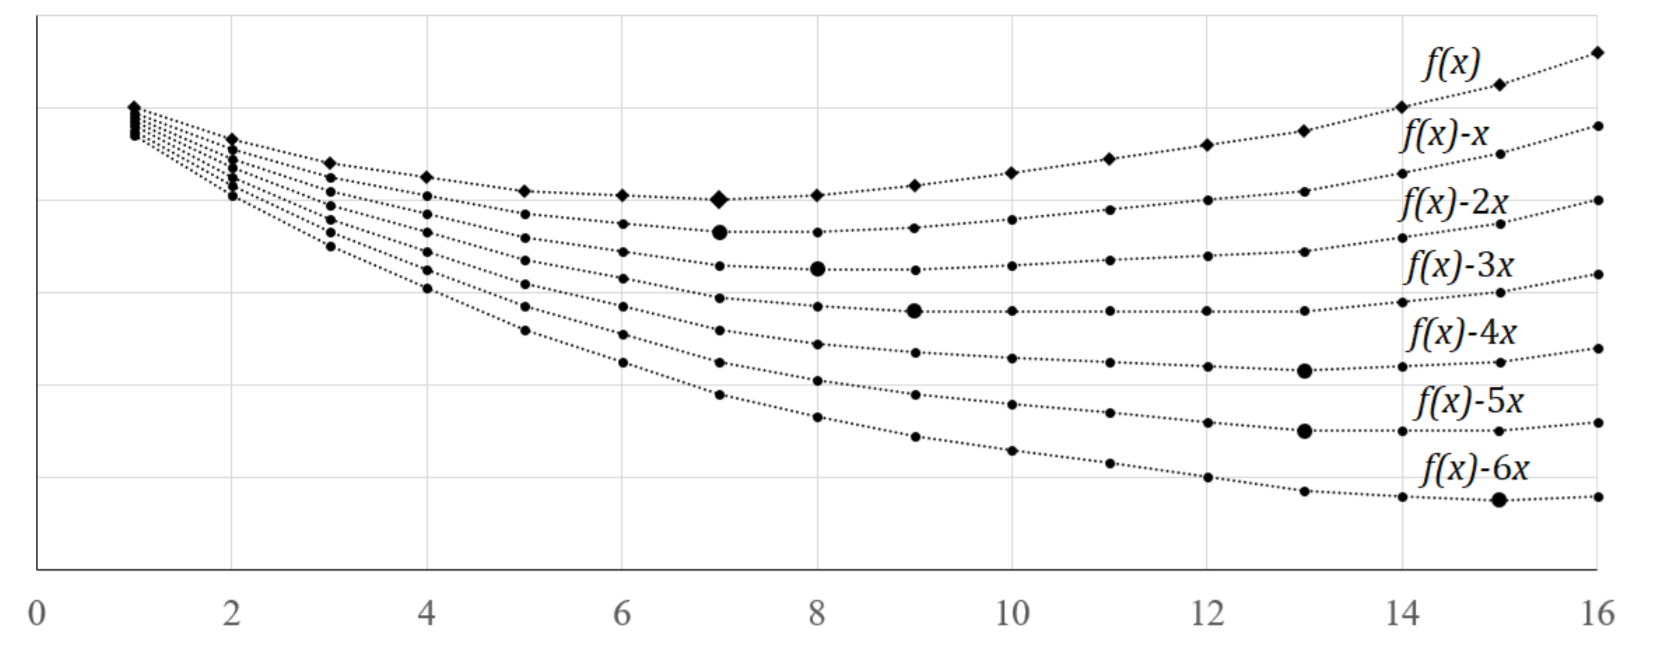
\includegraphics{aliensopt}
		\end{center}
		當然,可能會有一個問題出現:就是如果$p$的最小值出現在
	\section{四邊形不等式優化}
	
	所謂四邊形不等式優化,就是俗稱的打表找規律優化。為什麼這樣稱呼呢?因為四邊形不等式優化的滿足條件難以一眼看出  ,有些題目更是難以證明。前國手波路特石曾經說過:「我在選訓二模的時候,看到一題dp,我猜它是四邊形,就用原始的dp式打表找規律,最後AC了。」沒錯,四邊形不等式優化就是那麼玄妙的東西。
	
	\subsection{四邊形不等式與四邊形單調性}
	
	四邊形不等式優化之所以可以對轉移進行加速,是建立在\textbf{四邊形單調性}的基礎上。四邊形單調性是一個雙變數函數的性質,分為凹凸兩種。\\
	
	\definition{四邊形單調性}{
		函數$F$滿足\textbf{凹四邊形單調性},若對於任意的$i<i', j<j'$:\\
		如果$F(j, i) \leq F(j', i)$成立的話,必可以保證$F(j, i') \leq F(j', i')$。\\
		
		函數$F$滿足\textbf{凸四邊形單調性},若對於任意的$i<i', j<j'$:\\
		如果$F(j, i) \geq F(j', i)$成立的話,必可以保證$F(j, i') \geq F(j', i')$。
	}
	
	我們可以把$i$想像成時間,若$i$越大則越接近未來。那麼就可以把凹四邊形單調性想成:若此時(時刻$i$)的$j$比$j'$小,那未來(時刻$i'$)永遠都是$j$比較小。凸四邊形單調也可以用同樣的方式想:若此時$j$比$j'$大,那未來永遠都是$j$比較大。\\
	
	由於當你看到一個函數$F$時,你很難看出這個到底有沒有四邊形單調性,所以我們很常使用\textbf{四邊形不等式}來判斷這個函數的四邊形單調性。\\
	
	\definition{四邊形不等式}{
		\textbf{凹四邊形不等式:}
		
		如果對於任何$ i < i' \leq  j < j'$ 都有 $F(j, i) + F(j', i') \geq F(j, i') + F(j', i)$,則 $F$ 滿足凹四邊
		形單調性。\\
		
		\textbf{凸四邊形不等式:}
		
		如果對於任何$ i < i' \leq  j < j'$ 都有 $F(j, i) + F(j', i') \leq F(j, i') + F(j', i)$,則 $F$ 滿足凸四邊
		形單調性。\\
		
		如果這邊的$i, j$都是整數的話,我們只需要檢查$F(j, i) + F(j + 1, i + 1)$ 和$F(j, i + 1) + F(j + 1, i)$ 的大小關係即可。
	}
	
	滿足四邊形不等式的條件又稱為Monge condition,若一個函數滿足凸四邊形不等式,則必滿足凸四邊形單調性;若一個函數滿足凹四邊形不等式,則必滿足凹四邊形單調性。但是不滿足四邊形不等式的函數不一定沒有四邊形單調性,所以這時候,打表就是你的好幫手了。\\
	
	\problem{四邊形單調性}{
		數學題 - 判斷下列函數是否有凹四邊形單調性:
		\begin{enumerate}
			\item $F(x, y) = xy$
			\item $F(x, y) = (x-y)^2$
			\item $F(x, y) = s_x - t_y$,$s, t$是遞增數列
			\item $F(x, y) = (s_x - s_y)^2$,$s$是遞增數列
			\item $F(x, y) = aA(x, y) + bB(x, y)$,$a, b \geq 0$,$A, B$有凹四邊形單調性
			\item $F(x, y) = (x - y - 1 - K + \sum\limits_{k=x+1}^y C_k)^2$,$C$是正整數數列,$K$是正整數
			\item $F(x, y) = -a_x + a_y - \sqrt{y-x}$,$a$是正整數數列
		\end{enumerate}
	}
	
	\subsection{1D/1D 凸性優化}
	
	這邊要先來個簡單的名詞定義。如果我們說一個dp是$eD/tD$的,代表這個問題有$O(N^e)$個子問題,每個子問題需要$O(N^t)$的時間轉移,所以一個$eD/tD$的dp的總時間複雜度是$O(N^{e+t})$。
	
	\subsubsection{主要思維}
	
	說了這麼多,那四邊形單調性可以幹嘛呢?我們看看以下dp式:
	
	\begin{displaymath}
	dp[i] = \min\limits_{0\leq j < i} \{dp[j] + w(j, i) \}
	\end{displaymath}
	
	這種類型的dp可說是再熟悉不過了,這就是枚舉分段點再加上cost的題型。我們令$F(j, i) = dp[j] + w(j, i)$,如此一來我們在計算每個$dp[i]$時事實上就是在找$F(j, i)$最小的$j$。\\
	
	如果知道$w(j, i)$滿足凸四邊形單調性,那麼$F(i, j)$也會具備凸四邊形單調性,於是就可以套用四邊形不等式優化。\\
	
	1D/1D四邊形不等式凸性優化的精髓在於:如果在某個$i$時,$F(j, i)$比$F(j', i)$大(這裡的$j < j'$),那麼對於所有的時刻$i' > i$永遠都是$F(j, i)$會比較大,所以只要有一時刻從$j'$轉移比從$j$轉移好,就會導致不管未來何時,$j'$一定比$j$好,所以就可以永遠不用從$j$轉移了。\\
	
	\hint{
		我們可以得到一個結論:
		對於所有$i < i'$,$dp[i]$與$dp[i']$的最佳轉移來源$p_i \leq p_{i'}$。(轉移點單調)
	}
	
	我們引述一句蕭電的話:\\
	
	\eeric{
		這與斜率優化的精神很像,就是限制轉移來源。斜率優化用的是斜率單調性,而四邊形則是隨著$i$的遞增,轉移點也會遞增。我們可以用這個遞增的性質來加速轉移過程。
	}
	
	\subsubsection{實作方式}
	
	以下內容會有一些符號約定,這邊先列出來讓讀者更好理解:\\
	\definition{小約定}{
		$i$:時間點,當時間點是$i$就代表你正在計算$dp[i]$的值。\\
		$j$:轉移點,若我說時間點$i$時$j=$某數字就代表$dp[i]$從$j$那裡轉移。\\
		$p$:最佳轉移點,$dp[i]$的最佳轉移點會寫成$p_i$。\\
		$n$:就是$n$,也就是$i$的最大值。
		
		如果出現$i, i', j, j'$,通常表示$i < i'$,而且$j < j'$。
	}
	
	回歸到最原始的dp實作方式,我們在最外層的迴圈跑$i$,而內層迴圈枚舉轉移來源,看看哪個$j$可以使得$F(j ,i)$ 最小,來達到計算每個$dp[i]$的目的。\\
	
	現在套用了四邊形不等式優化,基本計算順序還是不變的,一樣是用一個迴圈跑$i$,逐步把$dp[i]$算出來。不過對於每個$i$都枚舉轉移來源$j$找最好的實在太慢了,就改成用集合維護一些區間,方便以$O(1)$查詢最佳的轉移來源。\\
	
	我們可以把區間$[1, n)$拆成許多不相交的小區間放進集合裡,集合裡的每個元素以$(p, L, R)$的方式儲存。若在時間點$i$時,集合裡面有元素$(p, L, R)$,就代表算到目前為止對於$L\leq i' < R$的$i'$,$dp[i']$的最佳轉移來源就是$p$,也就是說當$i$介於區間$[l, r)$內,則$F(p, i)$就不會比其他$k \not=p$的$F(k, i)$來的大。\\
	那麼我們要怎麼維護這個集合呢?我們考慮以下演算法:
	\begin{enumerate}
		\item 一開始除了$dp[0]$沒有任何$dp[i]$被算出來,所以區間$[1, n)$目前能確定的最佳轉移來源只能是$0$,因此先在集合裡放入區間$(0, 1: n)$。
		\item 當要計算$dp[i]$時,先把右界$R \leq i$的區間從集合中移除(因為這些區間已經不會再被用到了),然後再取右界最小的區間(此區間必包含$i$),從這個區間的$p$處轉移計算$dp[i]$。
		\item 當你計算出了$dp[i]$,那麼之後某些$dp[i']$的最佳轉移來源有可能因此更新成了$i$。這時候因為我們知道$i'$變大時$p_{i'}$只可能不變或變大,所以可以找到一個點$i^*$,使得所有大於等於$i^*$的$i'$的最佳轉移來源統統變成$i$。
		\item 找到這個$i^*$的方法如下:我們考慮右界最大的區間$(p_f, L_f: R_f)$
		\begin{enumerate}
			\item 若$F(i, L_f) \leq F(p_f, L_f)$,則這個區間的最佳轉移來源都即將被$i$取代,所以可以直接將區間拔掉,再考慮右界第二大的區間。
			\item 若$F(i, R_f) \geq F(p_f, R_f)$,恭喜你,什麼事都不用做,因為$p_f$目前還是最好的。
			\item 如果不是上述兩種情況,必然能在這個區間裡找到$i^*$,我們只要二分搜找到$F(i, k) < F(p_f, k)$的最小$k$,就是$i^*$。再從這個$i^*$將區間切成兩段$(p_f, L_f, i^*)$ 與 $(i, i^*: n)$即可。
		\end{enumerate}
	\end{enumerate}
	
	由於這些步驟每次只需要取得右界最大或右界最小的區間,並且放入區間時只會改變到右界最大的區間,所以可以用\inline{deque}來維護這個集合。\\
	
	實作方式與細節如下:(感謝baluteshih)\\
	
	\begin{C++}
		struct seg{int p,l,r;};
		deque<seg> deq;
		void solve(){
			deq.push_back(seg{0,1,n});
			for(int i=1; i<n; i++){
				// 計算dp[i]
				while(deq.front().r <= i) deq.pop_front();
				dp[i] = f(deq.front().p, i);
				// 更新以 i 作為轉移來源的區間
				while(deq.size() &&
				f(i, deq.back().l) < f(deq.back().p, deq.back().l))
				deq.pop_back();
				seg new_seg = seg{i, i+1, n};
				if(deq.size()){ // 有可能全部被 pop 掉
					int c = binary_search(deq.back().p, i);
					// c 是滿足 f(i, k) < f(deq.back().i, k) 的最小 k
					deq.back().r = new_seg.l = c;
				}
				if(new_seg.l < n) deq.push_back(new_seg);
			}
		}
	\end{C++}
	
	當然,你要先確定你的函數$F$有凸四邊形單調性。
	
	\subsection{1D/1D 凹性優化}
	
	凹性優化的題目十分罕見,不過還是有凹性優化的實作方式。\\
	
	與凸性優化的概念一樣,只不過相較於凸單調性,凹單調性可以推知:對於所有$i < i'$,$dp[i]$與$dp[i']$的最佳轉移來源$p_i \geq p_{i'}$。\\
	
	所以我們可以把凸性優化的\inline{deque}改成用\inline{stack}維護由上到下是$p$遞減(也就是區間遞增),每次插入一個新區間的時候因為裡面的所有$p$都比較小,所以會先動到(可能pop)數字大的。故top處放右界最小的區間,計算$dp$值時從top處pop掉不會再被用到的區間,然後選擇右界最小的區間轉移,每算完一個$dp[i]$,一樣從top處慢慢pop,再用二分搜找到$i^*$,不過因為是凸單調性,所以這裡的區間要拆成$(i+1, i^*)$與$(i^*, L_f)$兩部分。\\
	
	實作細節與凸性優化差不多,這邊就不列code了。
	
	\subsection{2D/1D 凸性優化}
	
	2D/1D 就是狀態二維,但轉移只有一維的dp,一般來說會長這樣:
	
	\begin{displaymath}
	dp[i][j] = \min\limits_{i\leq k < j} \{ dp[i][k] + dp[k][j] + w(i, j) \}
	\end{displaymath}
	
	這邊與1D/1D一樣,假設$w(i, j)$符合凸四邊形單調性,那麼通常$dp[i][j]$就滿足凸四邊形單調性。所以這邊可以枚舉$i$,讓dp狀態變成一維,就可以用$N$次的1D/1D解決,時間複雜度$O(N^2\log N)$。\\
	
	\hint{如果 $w(i, j)$ 為凸單調性的且 $w(i, i + 2) \geq \max(w(i, i + 1), w(i + 1, i + 2))$,則 $dp[i][j]$ 也會符合凸單調性}
	
	2D/1D凸性優化還有一個神奇的性質,不僅可以增加效率、降低時間複雜度,還可以大大的減低實作難度。\\
	
	這邊要介紹一個定理:\\
	
	\theorem{2D/1D 凸性優化}{
		設 $p_{i,j}$ 是 $dp[i][j]$ 在轉移時所找到的最佳轉移點,且 $dp$ 滿足凸四邊形不等式,則:
		\begin{displaymath}
		p_{i, j − 1} \leq p_{i, j} \leq p_{i + 1, j}
		\end{displaymath}
	}
	
	神奇的證明如下:先假設$p_{i, j-1} = k_1$,$p_{i, j} = u$,$p_{i+1, j} = k_2$,我們使用反證法,分兩邊討論:
	
	\begin{enumerate}
		\item 假設$k_1 > u$,則 $u+1 < k_1+1 \leq j-1 < j $,根據四邊形不等式可以得到:
		\begin{displaymath}
		dp[u+1][j-1] + dp[k_1+1][j] \leq dp[u+1][j] + dp[k_1+1][j-1]
		\end{displaymath}
		再利用$u$是$dp[i][j]$的最佳轉移來源的性質,可以列出以下式子:
		\begin{displaymath}
		dp[i][u] + dp[u+1][j] \leq dp[i][k_1] + dp[k_1+1][j]
		\end{displaymath}
		將以上兩不等式相加,可得:
		\begin{displaymath}
		dp[i][u] + dp[u+1][j-1] \leq dp[i][k_1] + dp[k_1+1][j-1]
		\end{displaymath}
		但這樣一來$k_1$就不是$p_{i, j-1}$了(因為選$u$的話更好),所以$k_1 \leq u$。
		
		\item 再假設$u > k_2$,可以用同樣方法,利用 $i < i+1 \leq k_2 < u $,列出四邊形不等式,再用$k_2$是$dp[i+1][j]$的最佳轉移來源,列出$dp$從$k_2$轉移與從$u$轉移的比較,最後再將兩不等式相加,就可以推出$u \neq p_{i, j}$的矛盾,因此$u \leq k_2$。
	\end{enumerate}
	
	如此一來我們得到了$k_1 \leq u \leq k_2$,定理得證。
	
	\subsubsection{實作}
	
	根據上述定理,我們可以發現到:$dp[i][j]$ 的轉移來源可以從區間 $[p_{i,j−1}, p_{i+1,j} ]$ 這個區間內找到,如果我們先計算$i-j$較小的$dp[i][j]$,並且記錄最佳的轉移點的話,枚舉範圍縮小了,就可以減少許多枚舉時間。\\
	
	那麼總共會省多少時間呢?我們可以考慮計算完一個 dp 表格的斜排 (也就是 $j - i$ 固定) 所需的時間:
	
	\begin{displaymath}
	\vdots
	\end{displaymath}
	\begin{displaymath}
	p_{i−2,j−3} \leq p_{i−2,j−2} \leq p_{i−1,j−2}
	\end{displaymath}
	\begin{displaymath}
	p_{i−1,j−2} \leq p_{i−1,j−1} \leq p_{i,j−1}
	\end{displaymath}
	\begin{displaymath}
	p_{i,j−1} \leq p_{i,j} \leq p_{i+1,j}
	\end{displaymath}
	\begin{displaymath}
	p_{i+1,j} \leq p_{i+1,j+1} \leq p_{i+2,j+1}
	\end{displaymath}
	\begin{displaymath}
	p_{i+2,j+1} \leq p_{i+2,j+2} \leq p_{i+3,j+2}
	\end{displaymath}
	\begin{displaymath}
	\vdots
	\end{displaymath}
	
	看出來了嗎?中間那行是同一個斜排的不同$dp[i][j]$的轉移來源,這些轉移來源的區間正好是連續的並且這些轉移來源會隨著$i$遞增而遞增,所以計算一個斜排所需的時間僅僅是$O(N)$!一個狀態2D的dp表格頂多$O(N)$個斜排,所以總時間複雜度$O(N^2)$!\\
	
	這邊是2D/1D凸性優化的核心代碼:\\
	
	\begin{C++}
		for(int len = 2; len <= n; len++){  // 枚舉區間長度 (i - j)
			for(int i = 1, r = len; j <= n; i++, j++){
				// 枚舉長度為 len 的所有區間
				dp[i][j] = INF;
				for (int k = p[i][j-1]; k <= p[i+1][j]; k++)
				if (dp[i][j] > dp[i][k] + dp[k+1][j] + w(i, j)){
					// 更新 dp 陣列
					dp[i][j] = dp[i][k] + dp[k+1][j] + w(i, j);
					p[i][j] = k;  // 記錄(最小)轉移來源
				}
			}
		}
	\end{C++}
	
	\subsection{2D/1D 凹性優化}
	
	凹性沒有好性質 QQ\\
	
	所以只能枚舉$i$,讓dp狀態變成一維,用$N$次的1D/1D解決了。時間複雜度$O(N^2\log N)$。
	
	\subsection{習題}
	\problem{超大畫框設置(TIOJ 1283)}{
		給定一個類似這樣的多邊形:(線皆垂直,且上面為右下右下⋯⋯,下面為下右下右下右⋯⋯),請問裡面可以放的最大矩形面積為何?(總邊數$\leq 10^5$)
		\begin{center}
			\includegraphics[width=0.5\textwidth]{1283_1}
		\end{center}
		
	}
	\problem{AI-666 賺多少(TIOJ 2039)}{
		你想要在股市賺錢:總共有$T$天,每天股市都有一個價格為$V_i$,你可以做買入或賣出,但是有一些限制:
		\begin{itemize}
			\item 只能先買後賣,不可以先賣後買。
			\item 每次買與賣都限定是一個單位的商品。同時,在買入之後,賣出之前,不可以再買入。
			\item 由於法令的規定,在此期間內最多只能進行$K$次的交易(一次交易包含買賣各一次)。
		\end{itemize}
		給定$T, V_i, K$,請問能得到的最大獲益為何?($K \leq N \leq 2 \times 10^6, V_i \leq 10^7$)
	}
		
			
%	\chapter{離線處理淺談 - 強大的工具}
如果一個演算法在計算答案之前不需要知道所有輸入,我們稱這個演算法為\textbf{在線}演算法;
反之若在計算答案的時候要先知道所有輸入,我們稱此為\textbf{離線}演算法。
例如插入排序在排序所有數字時可以一個一個讀進來再各自插入,選擇排序則是必須先讀進所有數字後,才能按照順序把最小的數字放到前面。


犧牲了即時更新性所換來的通常是計算量或coding複雜度的減少,我們先以 RMQ 當作一個簡單的例子。
\problem{經典題 - RMQ (ZJ d539)}{
給定一個序列 $a_1, a_2, \dots , a_n$,之後有 $q$ 次詢問 $[l,r]$ 中的最大值。 $n,q\leq 10^5$。
}
我們可以讀進所有詢問$[l,r]$,並依照左界由大到小排序。
如此一來,對於固定的左界只需要維護一個前綴max就足以回答所有詢問,
我們可以想到用 BIT 來維護這個東西,對於左界的遞減剛好對應到單點更新,
就這樣輕鬆完成不須線段樹的 RMQ 啦!雖然這個例子可能不一定能感受到離線演算法的威力,
但大家應該了解到了,如果離線計算的話可以用很多奇怪的方法去減輕時間、空間或coding複雜度。

\section{莫隊(Mo's Algorithm)}
從前面的題目可以發現,在面對一些區間詢問的題目時,有時我們可以藉由將詢問以
某種方式排序來降低操作整體的複雜度,其中有一種演算法稱為\textbf{莫隊}。

莫隊演算法通常適用於那些當區間左右界稍微改變時,能以很小的代價維護新區間的題目,
簡單來說,我們要想辦法排序詢問使得兩兩之間的「距離」都很相近,讓我們可以從前一個詢問的答案用不多的時間推出後一個詢問的答案以節省時間複雜度。
如果能花$F(n)$的時間從$[l,r)$的答案推到$[l\pm 1,r)$或$[l,r\pm 1)$,由$[l_1,r_1)$的答案推出$[l_2,r_2)$的答案所需要的時間就是$F(n)\cdot(|l_2-l_1|+|r_2-r_1|)$,這也可以看成座標平面上兩點的曼哈頓距離,我們可以用曼哈頓最小生成樹的演算法達到最差$O(F(n)\cdot n\sqrt{q})$的複雜度,但是否有更簡單的方法能達到相同的複雜度呢?

我們可以想到先將詢問依照左界排序,這樣當我們要查詢時左界只需要修改最多 $O(n)$,
不過聰明的大家應該會發現右界的順序是亂的!這就會導致我們的修改次數最多會退化至 $O(nq)$,
為了解決這個問題,我們決定也以某種方式對右界排序。

\textbf{我們把原序列分成 $m$ 塊 (每塊有 $n/m$ 個元素),並且依照左界所在的塊排序,若在同一塊則以右界排序。}
左界在同一塊間的移動次數總和最多就是 $q\cdot n/m$,而不同塊之間的移動次數最多是 $m\cdot 2(n/m) = 2n$;
右界在同一塊間的移動次數總和最多是 $nm$ ,而不同塊之間右界的移動次數最多也同樣是 $nm$;
因此總複雜度為 $O(F(n)\cdot (nq/m+nm+2n))$,可以發現取 $m=\sqrt{q}$ 會得到最佳複雜度 $O(F(n)\cdot n\sqrt{q})$ ,這也和曼哈頓最小生成樹可得到的結果相同,我們通常採用這種寫法。
莫濤提出的莫隊算法,除了將詢問排序之外,剩下都只是暴力計算,但是就是因為把詢問好好排序,得以把複雜度降低了一個根號。

實作上有一些細節,就是在更新左、右界時,盡量不要讓右界比左界小(也就是不要讓區間不合理),這部分的程式碼通常會用數個\inline{while}來實現,其架構大概長的像下面這樣。

\begin{C++}
struct Query{
	int l, r, id, block;
} Q[MAXQ];

bool cmp(Query &a, Query &b){
	return (a.block!=b.block) ? a.block<b.block : a.r<b.r;
}

int n, m, res, ans[MAXQ];
void add(int pos){ ... } // 維護增加一個數的改變
void sub(int pos){ ... } // 維護減少一個數的改變

void MO(){
	int K = 400; // 有時會依範圍直接寫一個固定的大小
	for(int i = 0; i < q; i++) Q[i].block = Q[i].l/K;
	sort(Q, Q+q, cmp); // 有時沒排序也沒過(X
	// 初始化也很重要,要注意一開始的區間
	int l = 1, r = 0;
	for(int i = 0; i < q; i++){
		// 先擴展再縮減
		// 這邊是左閉右閉的區間寫法,邊界問題自己要注意
		while(l > Q[i].l) add(--l);
		while(r < Q[i].r) add(++r);
		while(l < Q[i].l) sub(l++);
		while(r > Q[i].r) sub(r--);
		ans[Q[i].id] = res;
	}
	for(int i = 0; i < q; i++) cout << ans[i] << '\n';
}
\end{C++}

雖然莫隊通常是用來解決不帶修改的題目,但大陸人也有研發出可以解決待修改問題的莫隊,想法大概是把時間視為第三個維度,變成三維曼哈頓距離的感覺(前提是要能在時間軸上前後移動),用類似的方法可以有 $O(n^\frac{5}{3})$ 的複雜度。
\section{操作分治}
操作分治,又名 CDQ 分治。既然名字裡面有個分治,顧名思義就是利用了 Divide \& Conquer 的算法。
通常我們都希望問題的維度越低越好,但操作分治的做法卻是\textbf{加上了一個時間維度,
對時間分治,並保持其中一個維度有序},使問題的維度由 $n$ 到 $n+1$ 再降到 $n-1$。

儘管這個想法聽起來莫名其妙,但在處理帶修改的可離線問題時非常有效。
尤其是原本是帶修改的二維問題(加上時間變成三維),可能可以透過操作分治降低複雜度。

實際上操作分治可以分為三個步驟 :
\begin{itemize}
\item 計算左邊區間的答案
\item 計算右邊區間不受左邊區間影響時的答案
\item 計算左邊區間對右邊區間的影響
\end{itemize}
注意這邊是對時間分治,所以左邊右邊代表了時間上的先後;而以上三個步驟的順序也可能會依照題目改變。直接上例題吧!
\problem{經典題(No judge)}{
一個二維平面上,有$n$次操作,每次操作可以在一個點上加上權重,或者詢問某個座標的左下角所有權重的和。 $n\leq 10^5, |x|,|y|\leq 10^9$。
}
離散化是不可避免的,但就算離散化後用二維 BIT 或線段樹依然會 MLE,我們嘗試用操作分治降低問題的維度。

首先依照對每個操作加上一個時間維度,並直接對其分治。對每個區間來說,左右兩個區間的答案會變為兩個子問題,因此我們需要處理的只有「左邊區間的修改」對「右邊區間的查詢」的影響。可以發現,如果按照 $x$ 座標排序好,我們就可以直接動態維護 $y$ 座標前綴和 (BIT) 以得到答案;實作上有點類似merge sort中merge的部分,下面的 code 大概顯示了如何運作。

\begin{C++}
Query Q[MAXQ];
void merges(int L,int M,int R){
	int i = L, j = M;
	vector<query> tmp;
	init(); // BIT
	while(i<M || j<R){
		if((j==R) || ((i<M&&Q[i].x<Q[j].x){
			if(Q[i].type == ADD)
				add(Q[i].y,1); // BIT
			tmp.push_back(Q[i++]);	
		}else{
			if(Q[j]].type == QRY)
				ans[Q[j].id] += query(Q[j].y); // BIT
			tmp.push_back(Q[j++]);
		}
	}
	for(int i=0;i<R-L;i++)
		Q[i+L] = tmp[i];
}
void CDQ(int l=0, int r=n){
	if(r-l == 1) return;
	int mid = l+(r-l)/2;
	CDQ(l,mid),CDQ(mid,r);
	merges(l,mid,r);
}
\end{C++}

每次把一個區間$[l,r)$的兩部份以 BIT 合併求解的複雜度是 $O((r-l)\log n)$ (在離散化的前提下),總時間複雜度$T(n)=2T(n/2)+O(n\log n)$ ,由主定理得知$T(n)=O(n\log^2n)$。

雖然這題可能也可以用動態開點四叉樹或其他奇怪的資料結構解決,但操作分治寫法在空間、coding複雜度都表現得很好,並且時間複雜度的常數也很小。

\section{整體二分搜}
讀到這裡的同學應該都了解什麼是二分搜了吧!二分搜的檢查有時會有些代價,而如果直接各自二分搜這些代價加起來會使複雜度爛掉,我們想辦法讓這些代價能夠共用而減輕複雜度,因此就誕生了\textbf{整體二分搜}的演算法,顧名思義就是整體一起進行二分搜。
\problem{經典題 - 靜態區間第 $k$ 小}{
給定一個序列 $a_1, a_2, \dots , a_n$,之後有 $q$ 個詢問 $(l,r,k)$ ,請對每個詢問輸出 $[l,r]$ 第 $k$ 小的數字。
}
區間第 $k$ 大可能在嵌套或持久化資料結構也會提到,但利用持久化線段樹的寫法空間複雜度很高(筆者寫了兩天還一直MLE,QAQ),也不是我們今天的主題。

類似於\inline{lower\_bound},考慮對答案二分搜:
每次詢問一個 $x$ 並檢查每個詢問區間有幾個數不大於 $x$ ,如此可以分成答案要比 $x$ 大及答案要比 $x$ 小的兩種詢問;
注意原序列的數也可以分成比 $x$ 大及比 $x$ 小的兩種,
因此能把原序列也分成兩部分,變為兩個子問題遞迴解決。

至於我們要怎麼知道每個區間有多少數不大於 $x$ 呢?
我們可以用 BIT 維護「 $\leq x$ 的數的個數」的前綴和,
如此對於右半部遞迴的前綴和只需要以原序列中大於 $x$ 的數修改前半部遞迴時的 BIT 即可,省下每次都重算原序列或重置BIT的時間複雜度。整體二分的核心程式碼大概長的像這樣(參考自日月卦長的部落格),當然不同題目一定會需要修改細節部分。
\begin{C++}
// 原序列的數可視為操作一起放進陣列
// V,L,R 是操作們的索引,傳遞 int 比傳遞物件效率好
void totalBinarySearch(int l,int r,vector<int> &V){
	int mid = l+(r-l>>1);	
	vector<int> L,R;
	// 將V中對應的原序列數及詢問以mid為界分到L,R
	split(V,L,R,mid);
	// 二分搜答案不大於 mid 的
	totBS(l,mid,L);
	// 在BIT中記錄不大於 mid 的數造成的影響
	update(L);
	// 二分搜答案大於 mid 的
	totBS(mid+1,R);
	// 復原操作,以免影響到之後的搜索
	undo_update(L);
}
// split的實作,利用BIT
void split(vector<int> &V,vector<int> &L,vector<int> &R,	int x){
	for(int id:V){
		if(...){ //是原序列數a_i
			if(a_i < x) {
				add(i,1); // BIT
				L.push_back(id);			
			}else R.push_back(id);
		}
	for(int id:V){
		if(...){ // 是詢問(l,r,k)
			int cnt = query(r)-query(l-1); // BIT
			if(cnt < x) L.push_back(id);
			else R.push_back(id);	
		}
	}
	// 離開時記得 undo 讓 BIT 和進來前相同
	undo_update(L);
	V.clear(); // 節省空間
}
\end{C++}

我們來簡單分析一下整體二分搜的複雜度:原序列和詢問都在遞迴樹中出現,每個原序列的數以及每一個詢問出現的次數都是樹高 $O(\log(n+q))$ ,也是 BIT 修改及查詢的時間複雜度,而每次 BIT 修改最多$O(\log n)$(在離散化的前提下),因此我們的均攤時間複雜度是 $O((n+q)\log n\log(n+q))$。整體二分搜的一個明顯優點是空間複雜度低,只有 $O(n+q)$ ,畢竟除了遞迴呼叫使用的空間外也只開了一條 BIT,想當然爾出題者可能藉由記憶體限制的方式強制離線,又因為 code 短且不需要實作持久化樹狀資料結構,因此整體二分在競賽中被廣泛使用。

另外,在這題中由於我們是利用 BIT 來維護,undo 的成本很低,因此可以輕鬆的以 DFS 的方式呼叫遞迴,但有時候對於一些資料結構要 undo 其實是很困難的(例如 DSU),這時候我們就需要用到 BFS 的技巧。每次操作只在資料結構中增加內容,當二分搜進入新的一層後再將整個資料結構重置,便能避免掉昂貴的 undo 操作。
\section{習題}
習題的唷
\problem{XOR and Favorite Number(CF 617E)}{給定 $k$ 及一個長度為 $n$ 的正整數序列 $s$ ,對於 $Q$ 次詢問 $l, r$ ,每次輸出 $[s_l,\dots s_r]$ 中有幾對 $(i, j)$ 使得 $s_i \oplus s_{i+1} \cdots \oplus s_j = k$,其中 $\oplus$ 代表 XOR 運算。 $n \leq 10^5; s_i, k\leq 10^6$。}
\problem{區間眾數(ZJ b417)}{給定一個長度為 $n$ 的正整數序列 $s$ ,對於 $m$ 次詢問 $l,r$,每次輸出  $[s_l,\dots s_r]$ 眾數的個數以及有幾種數字是眾數。$n,m\leq10^5,1\leq s_i\leq n$。}
\problem{區間逆序數對(TIOJ 1694)}{給定一個長度為 $n$ 的正整數序列 $s$ ,對於 $q$ 次詢問 $l, r$ ,每次輸出 $[s_l,\dots s_r]$ 逆序數對的個數。$n, q \leq 10^6$,$s_i \leq 10^9$。}
\problem{Coding Days (TIOJ 1840)}{給定一長度為$N$的序列以及$Q$筆操作, 每筆操作可能為下列兩種:
\begin{enumerate}
	\item \inline{1 l r k}: 請輸出區間 $[l, r]$ 中第 $k$ 小的值。
	\item \inline{2 p v}: 將序列中的第 $p$ 個值改成 $v$。
	\item \inline{3 x v}: 關於這項操作,詳細的內容請觀察題目敘述。
\end{enumerate}
$N \leq 50000, Q \leq 10000$,序列中的數皆可以用\inline{int}儲存。
}
\problem{Stamp Rally (Atcoder)}{給定一張 $N$ 個點、 $M$ 條邊的無向圖,每條邊編號為$1\~{}M$。有 $Q$ 次詢問 $(x,y,s)$ ,輸出最小的 $i$ ,使得存在分別以 $x$ 和 $y$ 為起點的兩條路徑,路徑上的邊編號都不大於 $i$,且兩條路徑上共有 $s$ 個不同的點(包含 $x,y$ ,可以經過重複的邊或點但不會重複算到)。
$N,M,Q\leq10^5$。
}

%	\chapter{根號算法}
\section{前言}
	「十則圍之、五則攻之、倍則分之」,這是孫子兵法中提到的,說要視面對敵人的多寡,要採用不同的策略。同樣地,如果題目給的範圍有不同的限制,可能需要不同的作法。有時,這個限制可可能會在題目中就給了;不過,有時候題目連這個都不會給!所以,就必須要自己來界定分離的標準了。這個方法有時候看起來很通靈,甚至很唬爛,但是經過分析之後是對的,時常能將複雜度的一個變數降為其根號,譬如一個$O(N^2)$的演算法其實經過一點巧思是$O(N\sqrt{N})$,雖然會比$\log$等級的演算法慢一些,但是通常實作複雜度低許多,是一個很實用的工具!

\section{種類壓大小}
	還是一樣,先看一個簡單的例題吧:
	\problem{詭異的詢問(No Judge)}{
		我有一個神秘函數$f(x)$。每次,你都可以詢問一個$x$,我就會回你$f(x)$的值。另外一個人會問你$Q \leq 10^6$個正整數$k_i$,代表你要回答說$f(k)$等於多少,而且保證$\sum^{Q - 1}_{i = 0} k_i \leq 10^8$。然而,我很不耐煩,所以你只能問我$1000$次的詢問。請好好利用這$15000$次的詢問,來回答另外一個人的$10^6$個詢問吧!
	}

	乍看之下,這題根本不可做——有$10^6$筆詢問,可能有$10^8$個不同的數字,而我只有$10^4$次的詢問,根本不可做!首先,會先想到說如果重複詢問的話,那就先把問過的東西存下來再回答就好啦!所以呢,現在的問題就變成:到底有多少個可能的詢問呢?不過,或許眼尖的你注意到了奇怪的限制:$\sum^{Q - 1}_{i = 0} k_i \leq 10^8$!這有什麼用呢?想要讓數字最多種,當然要讓詢問的數字越小越好,才比較不會超越所給的限制,才會有最多種的數字呀!所以,假設是有$n$種數字,則一定是依序詢問$1, 2, 3, \dots, n$才好,所以呢:
	\begin{align*}
		\frac{n(n + 1)}{2} &\leq 10^8\\	
		(n + 1)^2 &\leq 2 \times 10^8\\
		n &\leq \sqrt{2 \times 10^8} - 1 \approx 14141 < 15000
	\end{align*}
	也就是呢,最多有$14141$種相異個數字會出現,所以只要存下來就好了!運用這個技巧,可以推論出一個結論:
	\theorem{和與種類的不等式}{
		假設有一堆數字的和為$S$,則那些數字的種類數量的數量級為$O(\sqrt{S})$。
	}
	此定理的證明和上面是一樣的,這裏就不贅述了。

\section{不會有那麼多個吧!}
	在一個圖中尋找三角形是很經典的一個問題:
	\problem{尋找三角形(經典問題)}{
		給定一個有$N \leq 10^4$個點,$M \leq 10^4$個邊的圖,請問這個圖有幾個三角形?一個三角形的定義為一個無序的3-tuple $(u, v, w)$($1 \leq u, v, w \leq N$),使得那三個點兩兩有邊連接。
	}
	先直接丟唬爛的解:枚舉一個邊$(u, v)$,看$\text{deg}(u)$和$\text{deg}(v)$哪一個比較小(假設是$u$),那就直接硬枚舉所有與$u$連結的點$x$,並看$x$和$v$是否有沒有連結,如果有的話,就直接加一。這樣,每個三角形都會被數到三次,所以就輸出答案除以三就好了!這樣的複雜度是$O(NM)$,因為對於每一個邊,都有可能掃到每另外一個邊。所以呢,先寫看看,傳上去,可以拿個部分——什麼?!居然AC了?為什麼呀?一樣用根號算法中的分case方法來分析其複雜度。接下來我們稱度數小於$\sqrt{M}$的點作「輕點」,反之則稱為「重點」。接下來考慮每個點當「小點」(一條邊連接的兩個點中度數較小的那個)對複雜度的貢獻。首先如果是輕點當小點,那就太棒了!因為輕點的度數$\sqrt{M}$


	%%%%%%%%%%%%%%%%%%%%%%%%%%%%%%%%%%%%%%%%%%%%%%%%%%%
	%\begin{thebibliography}{99}
	%\bibitem[1]{ex}\verb|http://www.example.com/|
	%\end{thebibliography}
\end{document}